% !TEX root = src/bachelorArbeit/main.tex
\documentclass[german,report]{tudo-raumplanung-thesis-report}

\usepackage{cite}
\usepackage{url}
\usepackage{wrapfig}
\usepackage{needspace}
\usepackage{geometry}
\usepackage{layout}
\geometry{
    left=3cm,
    right=2cm,
    top=2cm,
    bottom=2cm,
    showframe=false
    %textwidth=8cm,  
    %marginpar=3cm
    }

\usepackage{helvet}
\renewcommand{\familydefault}{\sfdefault}

\usepackage[german]{babel}

\usepackage[]{graphicx}

% Provide your title
\title{Entwicklung einer Methodik zur optischen Analyse
spannkraftinduzierter Deformationen additiv gefertigter Bauteile}

% Author name(s)
% organised into two columns if more than 10 authors are provided
\storeauthors\authors{
    {Thieme, Niklas}
}

% Provide the examiners' names.
\storereviewers\reviewers{
    {Jun.-Prof.\ Dr.\ rer.\ nat.\ Great Examiner}
    {Prof.\ Dr.-Ing.\ Fantastic Examiner}
}

\begin{document}
%\centering

\newpage

\tableofcontents

\newpage

% 1_EinleitungMotivation_tex
\chapter{Einleitung}

In den letzten Jahren hat die additive Fertigung (AF), auch bekannt als 3D-Druck, 
zunehmend an Bedeutung in der Industrie gewonnen~\cite{JADHAV20222094}. 
Diese innovative Technologie 
ermöglicht die schichtweise Herstellung komplexer Bauteilgeometrien und bietet im 
Vergleich zu traditionellen Fertigungsverfahren einen höheren Grad an 
Gestaltungsfreiheit. Trotz dieser Vorteile stehen Hersteller vor 
Herausforderungen bezüglich der Oberflächenqualität und Maßhaltigkeit 
der gefertigten Werkstücke~\cite{SCHNECK201919}.
Herausforderungen können die Bauteilgeometrie, die möglichen Materialien oder 
den Herstellungsprozess betreffen.
Die Herausforderungen bei der Bauteilgeometrie umfassen die minimalen 
Wandstärken sowie das maximale Bauteilvolumen, das von den technischen 
Spezifikationen des verwendeten 3D-Druckers abhängt. Für das (AF) stehen 
verschiedene Materialien zur Verfügung, 
die sich jedoch von den in der konventionellen, spanenden Fertigung 
verwendeten Werkstoffen unterscheiden. In der AF werden hauptsächlich Legierungen 
auf Basis von Titan, Aluminium, Nickel oder Chrom eingesetzt. Diese Materialien
müssen zudem in einer für das Verfahren geeigneten Form vorliegen, 
meistens in Form von Pulver oder Draht. Der Prozess zur Herstellung von 
Pulver oder Draht aus diesen Materialien ist kostenintensiv und schränkt
die Auswahl der verwendbaren Materialien ein. Aufgrund der 
schichtbasierten Natur der AF sind Stützstrukturen 
notwendig, um Bauteile mit geometrischen Formen, die Überhänge aufweisen, 
erfolgreich produzieren zu können. \label{drawbacks_af}
\cite{Vranic.2017}

Einige dieser Herausforderungen, können durch Nachbearbeitung des Bauteils 
gelöst werden. Dazu gehört das Entfernen der Stützstrukturen und die Verbesserung
der Oberflächenqualität.
Für den Nachbearbeitungsschritt muss das Bauteil in seiner Position und Lage im Bauraum
der Werkzeugmaschine fixiert werden. Die hierzu aufzubringenden Spannkräfte 
können die filigranen Bauteile elastisch, in Extremfallen auch plastisch, verformen, 
sodass eine maßhaltige spangebende Nachbearbeitung verhindert wird. 
Um den Spannprozess und dessen Auswirkungen auf das Bauteil hinsichtlich 
der erzielbaren geometrischen Genauigkeit optimieren zu
können, ist eine Quantifizierung der spannkraftinduzierten Deformation notwendig.~\cite{newMethod}

Im Rahmen dieser Bachelorarbeit wird deshalb eine Methodik zum Erkennen und 
analysieren einer Deformation entwickelt. Das Ziel dieser Methodik ist es, 
mithilfe von optischen Informationen zu additiv gefertigten Bauteilen eine 
Deformation zu erkennen, wie sie zum Beispiel auftreten kann, wenn ein Bauteil 
in einem Schraubstock fixiert wird.

Das Verfahren soll auf verschiedenen Bauteilgeometrien anwendbar sein, daher werden 
möglichst wenig Annahmen über die Bauteilgeometrie getroffen.
Im Verlauf dieser Arbeit werden erst die theoretischen Grundlagen, die für die 
entwickelte Methodik notwendig sind dargestellt. 
Anschließend wird das Vorgehen der Methodik vorgestellt und die einzelnen 
Schritte erläutert. Das Verfahren besteht aus mehreren Schritten die sich in 
Datenerfassung, Datenaufbereitung, Stitchting und Deformationserkennung 
einteilen lassen.

Nach der Vorstellung des Verfahrens wird die Funktion der Methodik anhand eines 
Demonstratorbauteils das in einem Schraubstock fixiert und mit mehrere Kraftstufen 
angezogen wurde, validiert. Hier wird die erkannte Deformation bewertet und 
verschiedene Materialien und Herstellungsverfahren verglichen.

Ziel dieser Arbeit ist es zusätzlich, die entwickelte Methodik in einer einfach
benutzbaren Anwendung um zusetzten. Die Funktionsweise dieser Anwendung wird 
nach der Validierung der Methodik dokumentiert. Außerdem werden verschiedene 
Optimierungen dargelegt, die das Verfahren Zeit- und Speichereffizienter machen
und die Genauigkeit der Ergebnisse verbessern.

Zum Abschluss dieser Arbeit wird ein Fazit gezogen, in dem die erzielten 
Ergebnisse eingehend diskutiert werden. Zudem wird ein Ausblick auf 
mögliche zukünftige Entwicklungen und weiterführende Forschungsansätze gegeben.





\newpage

\chapter{Grundlagen und Stand der Technik}

Für den Prozess der Deformationserkennung sind grundlegende Kenntnisse der 
Additiven Fertigung sowie des 3D-Designs von Vorteil. In diesem Kapitel 
werden sowohl diese Grundlagen als auch der aktuelle Stand der Technik 
erläutert.

\section{Additive Fertigung}

Additive Fertigung (AF) ist unabhängig von dem Werkstoff ein Bereich, in dem viel
geforscht und innoviert wird. In fast jedem Industriebereich wird versucht, ein
bestehendes Design oder Modell zu optimieren und zu verbessern.
Sei es hinsichtlich Qualität oder Kosteneffizienz. AF bietet bei 
dieser Optimierung viele Vorteile gegenüber spanenden Fertigungsverfahren, da 
AF einen höheren Grad der Gestaltungsfreiheit bietet. 
AF ist eine Ressource, welche Benutzern ermöglicht, komplexe 
Bauteilgeometrien zu erstellen, ohne die Limitierung von konventionellen spanenden 
Herstellungsverfahren zu erstellen. 
Limitierungen von konventionellen spanenden 
Herstellungsverfahren kann ein hoher Materialverschleiß oder die Notwendigkeit von 
spezialisierten Werkzeugen sein.\ \cite{Vafadar.2021} 

Außerdem können mit additiver Fertigung Stückzahlen drastisch reduziert werden.
Werkstücke können bei Bedarf gefertigt werden, was die Notwendigkeit für Lagerstätten
größtenteils eliminiert. Zusätzlich können die Teile genau dort herstellt werden, wo 
sie benötigt werden, was Lieferketten und Wartezeiten verkürzt~\cite{Calignano.2023}.

Bauteile können mit verschiedenen Werkstoffen, darunter sind Polymeren, Metalle und Keramik, 
additiv gefertigt werden.
Metalle haben vor allem in den letzten Jahren 
an Relevanz gewonnen. Zusätzlich zu den schon genannten Vorteilen von AF, 
bietet Metall als Werkstoff großen Nutzen in der Industrie. Gegenüber Kunststoffen
produziert Metall weniger Abfall und kann eine höhere Qualität gewährleisten.
Zusätzlich dazu kommen die offensichtlichen Vorteile von Metall gegenüber Polymeren: 
höhere Hitzebeständigkeit und eine stabilere Grundstruktur, was sie weniger anfällig 
für Verformungen macht~\cite{Gardner.2023}.

Aufgrund dieser Vorteile wird AF in vielen Industriebereichen genutzt. Die folgende
Sektion zeigt einige Fälle in der Automobilindustrie, in denen AF 
erfolgreich benutzt wird.
Die Automobilbranche ist ein Bereich, in der AF schon viel und erfolgreich 
eingesetzt wird:
Durch AF könne Teile gefertigt werden, die leichter, belastbarer und sicherer sind. 
Die einfache Anpassbarkeit sorgt für geringe Entwicklungszeiten und Kosten. 
BWM zum Beispiel benutzt für den i8 Roadster viele AF gefertigte Teile.
Darunter sind zum Beispiel die Befestigung für das Soft-Top, die 44 \% leichter als das Spritzgussteil
ist, und dennoch zehnmal steifer.\ \cite{Vafadar.2021} 
Fensterführungen wurden auch additiv gefertigt. Mithilfe des \glqq HP Multi Jet Fusion\grqq~
konnten 
100 Teile in 24 Stunden gefertigt werden. Selbst Teile des Zylinderkopfs für den 
S58 Motor wurden additiv gefertigt. \cite{Anusci.2019}

Auch bei älteren Fahrzeugen können additive Fertigungsmethoden zur 
Reparatur oder Restauration verwendet werden.
Gerade bei älteren Fabrikaten sind Ersatzteile häufig nicht mehr vom 
Erstzulieferer zu beschaffen oder mit konventionellen Herstellungsmethoden
wirtschaftlich herzustellen.
Bei einem Matra 530 aus 1973 wurde zum Beispiel die rechte 
Kotflügelhalterung erfolgreich reproduziert, nachdem auch nach längerer Suche
kein Originalteil gefunden wurde \cite{AMExpo365.03.06.2024}. Zusätzlich war
bei diesem Beispiel die Herausforderung, das keine digitale Version des
Bauteils existiert hat. Zuerst musste also ein Modell als Grundlage für die
additive Fertigung erzeugt werden.

\section{Limitierungen von AF}

AF kann trotz seiner Vorteile nicht überall eingesetzt werden. Limitierungen 
in der Materialvielfalt, hohe Material und Anschaffungskosten, begrenzte
Bauraumgrößen, verminderte Oberflächenqualität und aufwändige Nachbearbeitungen
können einen Einsatz von AF verhindern beziehungsweise unwirtschaftlich machen. 
\cite{inproceedings}
Einige dieser Limitierungen können umgangen oder gelöst werden. 
Zum Beispiel kann die
verminderte Oberflächenqualität kann durch eine anschließende Fräsbearbeitung
verbessert werden. 
Diese Nachbearbeitung macht eine Fixierung des Bauteils notwendig. Auch für andere
Nachbearbeitungen wie das Entfernen von Stützstrukturen kann sich das fixieren
positiv auswirken und Zeit im Herstellungsprozess eingespart werden.
Wie schon in Kapitel \ref{drawbacks_af} beschrieben, sind 
Stützstrukturen notwendig, wenn das zu produzieren Bauteil Überhänge aufweist,
die eine Steigung von ungefähr 30° unterschreiten. Der Grad des Überhangs 
variiert je nach verwendetem Material und Verfahren.

\begin{figure}[H]
    \centering
    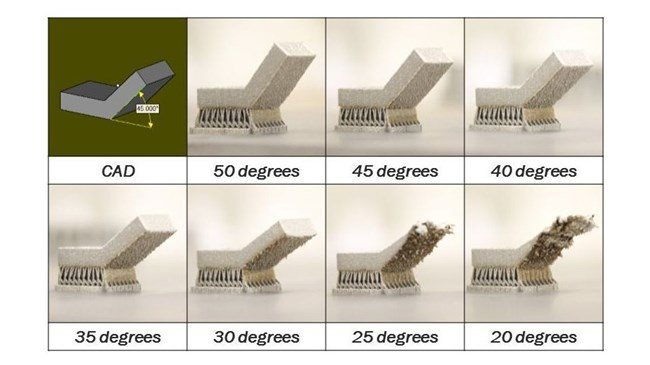
\includegraphics[width=0.9\linewidth]{images/Overhang-tests-showing-different-printabilities-and-finish-qualities-at-seven-different.jpg}
    \caption{Überhangtests mit unterschiedlichen Resultaten und 
    Oberflächenqualitäten in sieben verschiedenen Winkeln \cite{Meng.2020}}
    \label{fig:overhang}
\end{figure}

\section{Reverse Engineering}

Reverse Engineering beschreibt den Prozess aus einem bestehenden Produkt 
oder Objekt ein digitales Abbild zu erzeugen.
Dabei sind meistens wenig oder keine technischen Details über das Objekt
verfügbar.~\cite{Helle.2021}  
Auch wenn Baupläne vorhanden sind, kann es trotzdem notwendig sein, 
Reverse Engineering zu betreiben, denn das tatsächliche Produkt kann von
den Bauplänen abweichen. Produkte und Bauteile können durch die Benutzung 
abgenutzt werden und entsprechen deswegen unter Umständen nicht mehr den originalen 
Bauplänen. Zusätzlich können Toleranzen im ursprünglichen Fertigungsprozess 
für Diskrepanzen sorgen. Wenn technische Details vorhanden sind,
können diese aber im Reverse Engineering Prozess verwendet werden.\ \cite{Monchinger.2021} 
Dieses Paper zeigt, wie Reverse Engineering genutzt werden kann, um 
bestehende Bauteile passgenau zu erweitern. Konkret geht es um die
Entwicklung einer Methodik um automatisiert Laser-Scans und originale Baupläne
zusammenzufügen um ein möglichst detailgetreues Abbild der realen Struktur zu
erzeugen. Dieses Abbild wird dann benutzt, um die bestehende Struktur zu 
erweitern und auf ihr aufzubauen. Das wird am Beispiel eines Flugzeugs 
demonstriert, erst wird der Innenraum gescannt und mit dem originalen Plänen
abgeglichen, dann ein 3D Objekt erstellt. Mithilfe dieses 3D-Objekts können 
dann passgenaue Bauteile hergestellt werden, die es ermöglichen ein ehemaliges 
Passierflugzeug in eine Frachtmaschine umzubauen.
Wie schon erwähnt, wird zur erfolgreichen Weiterbearbeitung ein möglichst 
genaues digitales Abbild benötigt.
Ist dies nicht der Fall, müssen nicht passende Teile erneut hergestellt werden, 
was die Material- und Personalkosten deutlich erhöht. Es ist also im 
wirtschaftlichen Interesse beim ersten Schritt, dem Erstellen der digitalen 
Version, ein möglichst genaues Ergebnis zu erzielen. 

\section{3D Rekonstruktion}

Digitale Abbildungen von Flächen, Objekten oder sogar Körperteilen wurden in den
letzten Jahren mehr benutzt. Anwendungen sind zum Beispiel in der
geometrischen Dokumentation, Inspektion, Navigation, Visualisierung und 
Objekterkennung zu finden~\cite{Verykokou.2023}. Je nach Anwendungsfall wird eine
bestimmte Genauigkeit
der Daten erwartet, im medizinischen Bereich sind die Ansprüche natürlich ganz 
andere als zum Beispiel in der Dokumentierung von ganzen Gebirgszügen.
Das Scannen von Gesichtstexturen zeigte Abweichungswerte zwischen 140 $\mu$m und 
1330 $\mu$m, während die 3D-Rekonstruktion des Kieferknochens Werte zwischen 106 $\mu$m 
und 760 $\mu$m aufwies. 
Das Scannen eines bezahnten Bogens durch intraorale und Labor-basierte
Scanner variierte zwischen 17 $\mu$m und 378 $\mu$m und bei der 
digitalen Abtastung von Zahnimplantaten zwischen 19,32 $\mu$m
und 112 $\mu$m~\cite{Bohner.2019}.
Bei Lidar-Scans eines Sportkomplexes wurde eine Standardabweichung von ±0.10 Metern
gemessen. Es wurde aus 600 Meter Höhe vermessen und die Scandaten mit 
Referenzpunkten auf dem Boden verglichen.~\cite{Elaksher.2023}
Aus diesem Grund existieren auch verschiedene Herangehensweisen und Technologien  
zur 3D-Rekonstruktion.

3D Rekonstruktion-Technologien können in 2 Kategorien eingeteilt werden,
die bildbasierte Verfahren und die Verfahren die auf Scandaten 
beruhen.~\cite{Verykokou.2023} [TODO es existieren noch mind. 2 weitere verfahren]
Beide Verfahren können auch kombiniert werden. 
Bei bildbasierten Verfahren, auch Fotogrammetrie genannt, wird das 3D Objekt aus
mehreren zweidimensionalen Bildern erstellt, 
umso mehr Bilder vorhanden sind, desto besser kann das
3D Objekt rekonstruiert werden. Um das 3D Objekt zu erstellen werden in 
allen Bildern gemeinsame Punkte gesucht und dann mit der bekannten Kameraposition, 
die relative Position des Punktes im 3D Objekt ermittelt. Figur [todo figur einfügen] zeigt dies 
anschaulich.
Vorteil bei der Fotogrammetrie ist, dass die Daten relativ einfach aufgenommen werden
können. Die Kamera eines Smartphones kann ausreichend hochauflösende Bilder aufnehmen, um 
eine 3D-Rekonstruktion zu ermöglichen. Des Weiteren sind viele Softwarelösungen,
auch kostenlose, vorhanden um automatisiert 3D Objekte zu erzeugen.
Gründe, sich gegen den Einsatz von Fotogrammetrie zu entscheiden, 
liegen in der begrenzten Auflösung sowie im signifikant ansteigenden Arbeitsaufwand 
bei steigenden Anforderungen an die Genauigkeit des Endergebnisses. 
Fotogrammetrie zeigt jedoch ihre Stärken bei großflächigen 3D-Rekonstruktionen, 
wie sie beispielsweise bei der Erfassung von Gebäuden, Stadtteilen oder geografischen 
Strukturen erforderlich sind.

\begin{figure}[H]
    \centering
    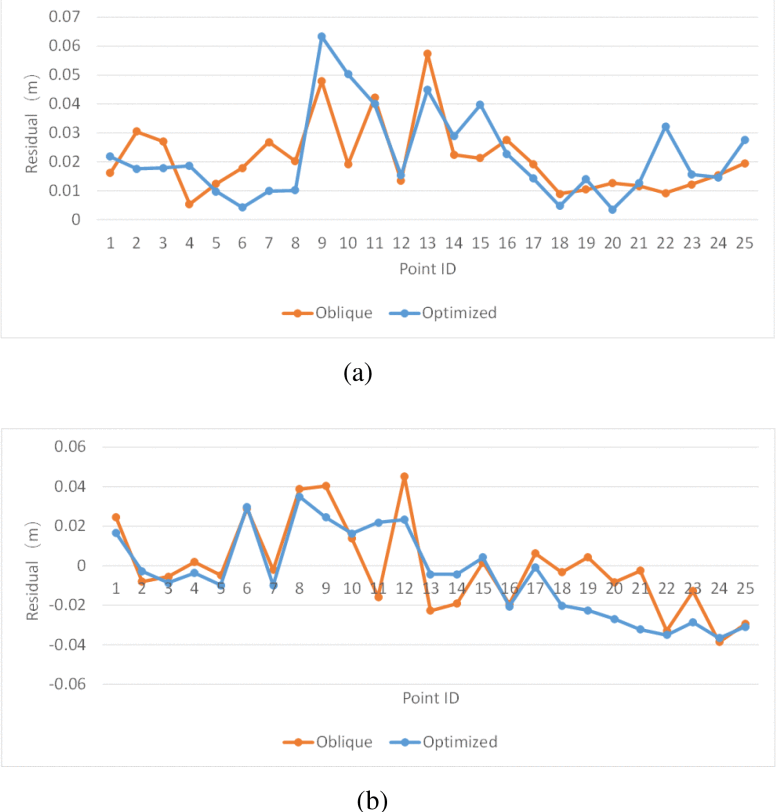
\includegraphics[width=\linewidth]{images/photogammatry_accurancy.PNG}
    \caption{Genauigkeit der Fotogrammetrie bei Bildern die aus 
    600 m Höhe aufgenommen wurden \cite{Elaksher.2023}.}
    \label{fig:photogammatryAccuracy}
\end{figure}

Für kleine Objekte, bei deren Rekonstruktion eine hohe Genauigkeit gefordert ist, 
sollte daher das zweite Verfahren angewendet werden. Bei diesem Verfahren werden
die Ursprungsdaten dreidimensional mit einem Scanner erfasst. Ein Scanner misst dabei, 
meist mithilfe von Lichtstrahlen, den Abstand zu einem Punkt auf dem zu 
rekonstruierenden Objekt. Um eine Vielzahl von Scanpunkten zu erfassen, 
wird entweder das Objekt oder der Scanner bewegt. Je mehr Punkte erfasst werden, 
desto genauer wird das Ergebnis. Allerdings nimmt die Datenmenge mit der Anzahl der 
Scanpunkte ebenfalls zu, was ab einem bestimmten Punkt zu einer Einschränkung durch den 
verfügbaren Speicher führen kann. Zudem steigt die Rechenzeit mit der Datenmenge an, 
und je nach angewendetem Verfahren kann dieser Anstieg sogar 
exponentiell sein~\cite{XiaoleiDu.2009}.

Nachteile von diesem Verfahren sind die hohen initialen Kosten eines Scanners 
und der begrenzte Messbereich. 

\subsection{Digitales Abbild}

Das schon vorhandene oder erstellte 3D Objekt muss für die weitere Nutzung
in einem geeigneten Datenformat gespeichert werden. Hierfür haben sich mehrere
Formate etabliert. Die Geometrie eines Objekts wird häufig als Sammlung von Punkten 
gespeichert. Die Oberfläche eines Objekts wird als Serie von Polygonen beschrieben. 
Der Grad des Polygons kann variieren, häufig werden Dreiecke verwendet. 
Die Genauigkeit, mit der das Polygon-Netz die gewünschte Oberfläche 
abbildet, kann gewählt werden. 
Je kleiner die Oberfläche der Polygonen ist, desto genauer wird die Oberfläche 
abgebildet. Mit kleineren Oberflächen steigt die Anzahl der zu speichernden 
Eckpunkte, was eine größere Datei zur Folge hat.
Ein in der akademischen Welt beliebtes Dateiformat für Polygon-Netze ist das 
Polygon File Format (ply).\ \cite{KentonMchenry.2008}
Das Format kann vom Nutzer beliebig angepasst werden. Eine ply-Datei beginnt mit 
einem Header in dem die Inhaltsstruktur beschrieben wird. 
Für 3D-Objekte besteht diese meistens aus X, Y und Z Koordinaten. 
Zusätzlich können weitere Informationen gespeichert werden. Das ply Dateiformat 
unterstützt standardmäßig: \glqq vertices/edges/faces, vertex colors, textures and
material \grqq ~\cite{KentonMchenry.2008}. Weitere Informationen können durch den Nutzer 
hinzugefügt werden, 
diese können dann aber unter Umständen nicht von anderen Programmen oder Benutzern
benutzt werden.
Im Dateiheader wird zu jedem Attribut auch der Datentyp festgelegt. Durch diesen 
kann die Genauigkeit und Dateigröße beeinflusst werden. Häufig werden hier Floats oder
Integer in verschiedener Bittiefe gewählt.

\begin{figure}[h]
    \centering
    \begin{minipage}{0.32\textwidth}
        \centering
        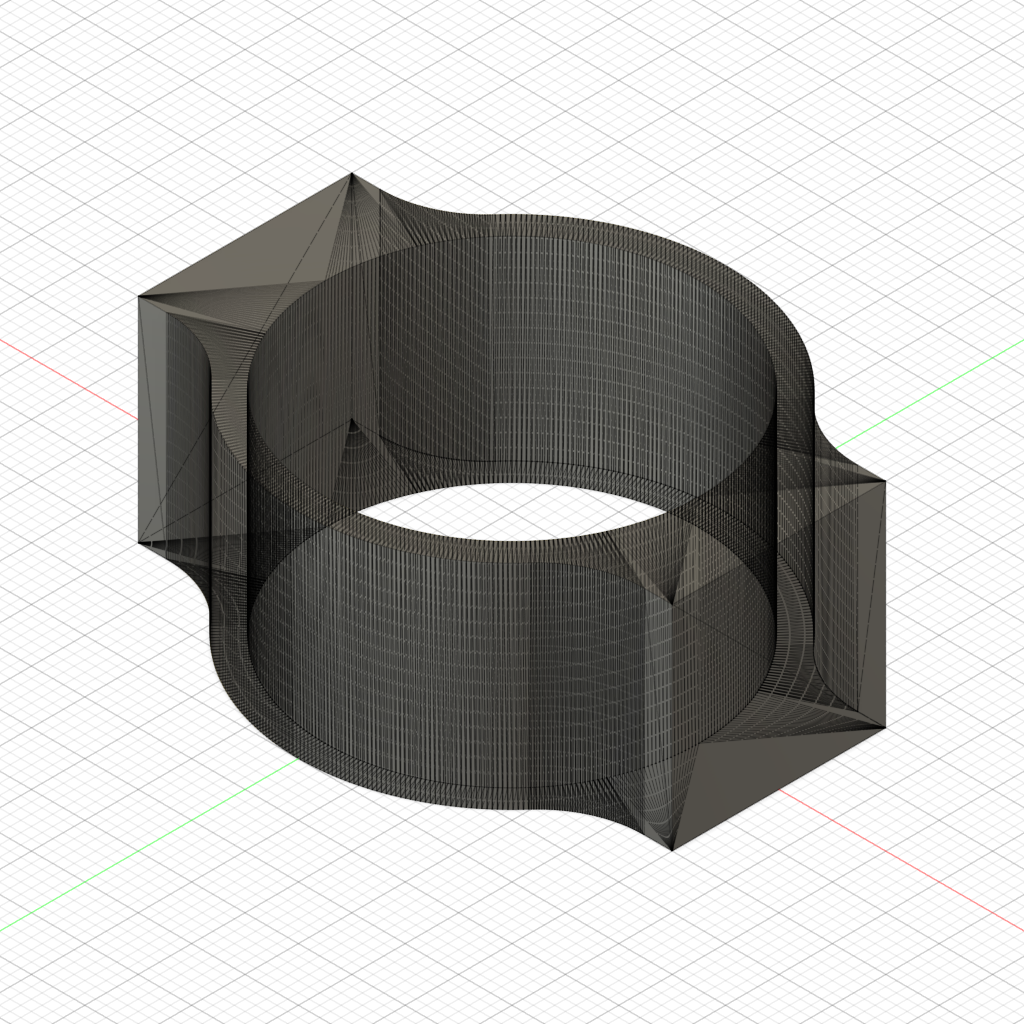
\includegraphics[width=\linewidth]{images/image_demo.PNG} % first figure itself
        \caption*{(a)}
    \end{minipage}\hfill
    \begin{minipage}{0.32\textwidth}
        \centering
        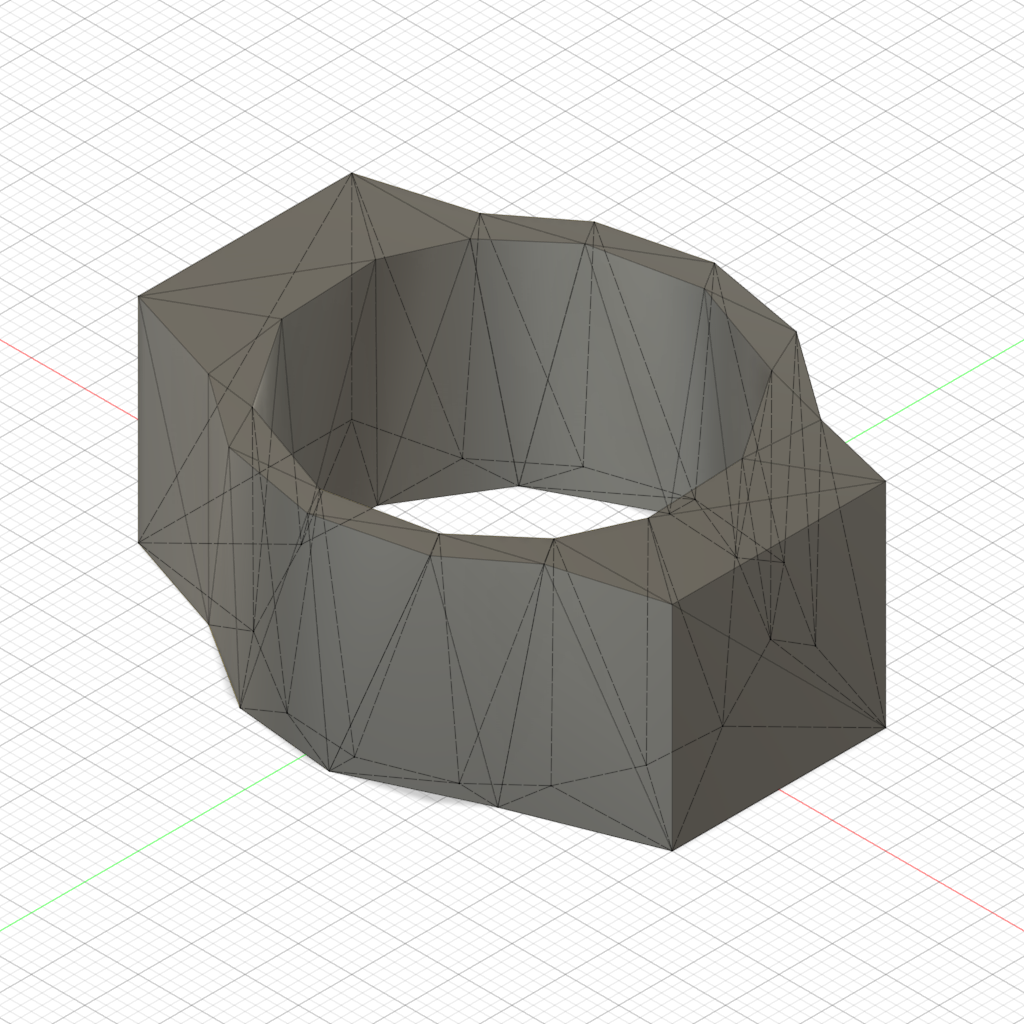
\includegraphics[width=\linewidth]{images/image_demo_medium.PNG} % first figure itself
        \caption*{(b)}
    \end{minipage}\hfill
    \begin{minipage}{0.32\textwidth}
        \centering
        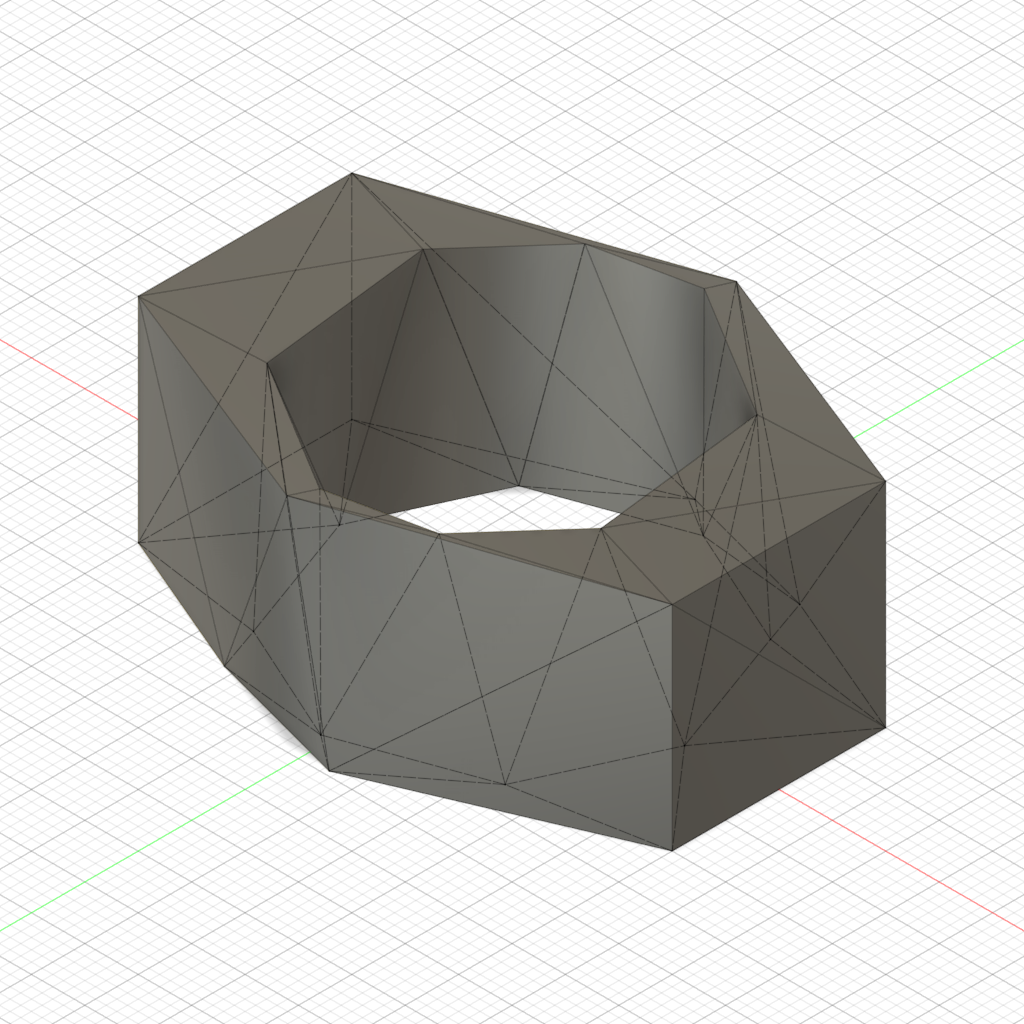
\includegraphics[width=\linewidth]{images/image_demo_low.PNG} % first figure itself
        \caption*{(c)}
    \end{minipage}\hfill

    \caption{Genauigkeit einer 3D-Datei ist abhängig von der Anzahl der gespeicherten
    Eckpunkte am Beispiel des Demonstratorbauteils. (a) 1512 Punkte
    (b) 52 Punkte (c) 30 Punkte}
    \label{fig:3d_design}
\end{figure}

\subsection{Scanner und Datenerfassung}
[todo verschiedene Scanner differenzieren und vergleichen]

Wie schon beschrieben, können dreidimensionale Daten direkt mit einem 
Scanner aufgenommen werden. 
Der Scanner hat, abhängig vom Modell und der angebrachten Höhe einen limitierten
Bereich, den er erfassen kann. 
Je nach Scannertyp und Modell kann sich der Messbereich ändern.
In Abbildung \ref{fig:scanner} ist ein Messbereich für den Scanner vom Typ 
ScanControl-LLT30xx sichtbar. Mittig kann 
in einer Tiefe von 85 mm eine Linie mit der Länge 25 mm gemessen werden. 
Der komplette messbare Bereich ist rot markiert. \cite{MESSTECHNIK_2020}
Bauteile die breiter sind als die maximale Breite der Scanebene, in Abbildung 
\ref{fig:scanner} mittig 25 mm, können also nicht in einer Pointcloud erfasst werden. 
Damit eine Digitalisierung von größeren Objekten erfolgen kann, müssen
also mehrere Scans durchgeführt, und später zusammengefügt werden. Zwischen den 
Scanvorgängen muss der Scanner in Richtung der Breitenachse verschoben werden.
Die Länge der Verschiebung sollte kleiner als die Scannerbreite sein, 
damit eine Überlappung entsteht, die 
genutzt werden kann, um die Pointclouds wieder zusammenzufügen. Die Verschiebung kann 
beliebig klein gewählt werden, jedoch steigt der Arbeitsaufwand und die Dateigröße mit 
jeder zusätzlichen Pointcloud, während das Ergebnis sich nicht verbessert.
Das Ergebnis verbessert sich nicht, da nicht mehr Daten aufgenommen werden, sondern nur 
die gleichen Daten mehrfach.
So können Pointclouds aufgenommen werden die dann in dem zu entwickelnde Verfahren
wieder zu einem digitalen Abbild zusammengefügt werden.

\begin{figure}[h]
    \centering
    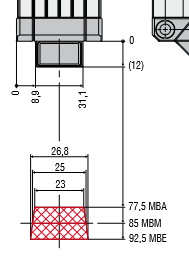
\includegraphics[width=0.3\textwidth]{images/Scanner.PNG}
    \caption{Funktionsweise eines Laserscanners [todo was ist abgebildet]}
    \label{fig:scanner}
\end{figure}

\section{Transformationen} \label{Transformation}

Eine Transformation ist eine Funktion, die eine Menge von Punkten in einem
Raum auf eine andere Menge von Punkten in demselben oder einem anderen Raum abbildet. 
Diese Transformationen werden verwendet, um die Lage, Form oder Größe von 
Objekten zu verändern.
Es gibt drei Basis Arten der Transformationen:
Translation, Rotation und Skalierung. Die Translation verschiebt alle Punkte 
um einen bestimmten Vektor in eine bestimmte Richtung. 
Rotation: Drehen eines Objekts um einen Punkt (in 2D) oder eine Achse (in 3D).
Veränderung der Größe eines Objekts durch Multiplikation der Koordinaten 
mit einem Skalierungsfaktor~\cite{XiaoleiDu.2009}.

\section{ICP-Algorithmus} \label{icp}

Der Iterative-Closest-Point-Algorithmus (ICP-Algorithmus) existiert schon seit dem Beginn der 90er Jahre und ist 
die klassische Methode, wenn es um die Registrierung von Pointclouds und 
anderen Punkt-Sets geht. \cite{icp}
Der Algorithmus errechnet eine lokale, optimale Transformation, die ein Daten-Set
dem anderen annähern kann. \cite{icp_og}
Um diese Transformation, zu bestimmen werden zuerst die Distanzen von allen 
Punkten in Daten-Set A zu dem jeweils nächsten Punkt in Daten-Set B aufsummiert 
werden. Dann wird eins der Daten-Sets verschoben und rotiert und wieder die 
Distanzen gebildet. Dies wird so lange gemacht bis die Änderung der Distanzen 
konvergiert. Die entstehende Transformation ist dann optimal.
Für identische Daten-Sets die sich nur in einer Transformation und Rotation 
unterscheiden, funktioniert dieser Algorithmus sehr gut. Bei Daten-Sets die 
Messfehler oder Überlappungen beinhalten kann häufig keine optimale 
Transformation bestimmt werden.
Deswegen wurden seit der ersten Vorstellung des Algorithmus viele Varianzen
entwickelt, die mit diesem Schwächen umgehen. 
Zum Beispiel der 'Sparse Iterative Closest Point' Algorithmus von~\cite{Bouaziz.2013}
oder die 'Anderson-accelerated' Version die besser mit Ausreißern und nur 
partiell überlappenden Daten umgehen kann und eine gleichwertige oder bessere 
Transformation errechnen kann.\ \cite{icp}
Der Algorithmus geht iterativ vor und berechnet immer eine optimale lokale Transformation.
Die beiden Daten-Set sollten schon vor dem Anwenden des ICP-Algorithmus grob angenähert sein, 
das beschleunigt die Konvergenz und damit die Laufzeit des Algorithmus.
Eine grobe Annäherung kann ermittelt werden, indem die Massenmittelpunkte der beiden Daten-Set
übereinander gelegt werden. In Abbildung \ref{fig:ipc_princip} ist das Prinzip visuell 
dargestellt. Die grünen Linien sind jeweils die kürzeste Distanz von Q nach R. 

\begin{figure}[h]
    \centering
    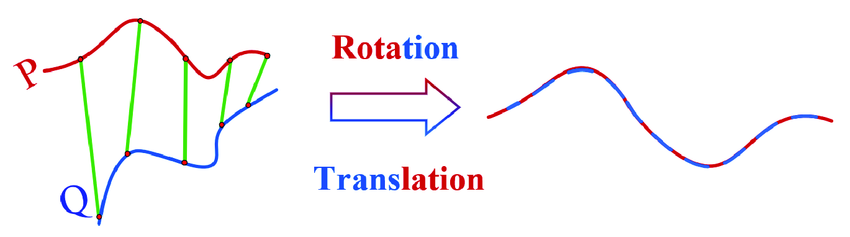
\includegraphics[width=0.7\textwidth]{images/Principle-of-ICP-algorithm.png}
    \caption{Prinzip des ICP-Algorithmus}
    \label{fig:ipc_princip}
\end{figure}



\newpage



\chapter{Ziel der Arbeit}

Wie schon beschrieben müssen additiv gefertigte Bauteile nachbearbeitet werden
bevor sie eingesetzt werden können. 
Um eine korrekte Nachbearbeitung gewährleisten zu können muss das additiv 
gefertigte Bauteil fixiert werden. 
Dies kann vorgenommen werden, indem das Bauteil in einen Schraubstock eingespannt wird.

\section{Einspannproblematik}

Durch das Einspannen kann das Bauteil so deformiert werden, dass die vorgesehene Nutzung nicht mehr möglich ist. 
Je nach verwendetem Werkstoff und Geometrie kann die Deformation unterschiedlich
ausfallen. 

\section{Erfassung der spannkraftinduzierten Deformation}

Für die Beurteilung, ob ein Bauteil noch eingesetzt werden kann, ist es nötig die 
Deformation die auf das Objekt gewirkt hat zu erkennen. Wenn das Bauteil in einen 
Schraubstock eingespannt wird, wirkt eine Spannkraft über die Backen des Schraubstock
auf das eingespannte Bauteil. 
Diese Kraft induziert eine Deformation auf das Bauteil. Diese Deformation soll 
optisch in einem Verfahren erkannt und dargestellt werden.

\section{Verfahren zur optische Spannkraftdeformationserkennung}

Um die Deformation des Bauteils erfassen zu können wird das 3D-Objekt benötigt, 
dass als Grundlage für die AF diente. Zusätzlich werden optische Daten des Bauteils 
im deformiertem Zustand benötigt. Mit diesen beiden Daten kann der Unterschied 
ermittelt und ausgegeben werden.
Um auch minimale Deformationen erkennen zu können müssen die Daten des 
eingespannten Bauteils hinreichend genau sein. Deswegen wird ein Laserscanner zur 
Datenerfassung eingesetzt.
Wie schon beschrieben ist der Messbereich eines Laserscanners begrenzt. Da das 
Verfahren nicht auf eine Bauteilgröße beschränkt sein soll, müssen mehrere Scans als 
Eingabe akzeptiert und damit umgegangen werden.

\section{Vorgehen}

Das Verfahren, um eine Deformation in einem eingespannten additiv gefertigten
Bauteil, zu erkennen umfasst folgenden Schritte:

\begin{itemize}
    \item \textbf{Digitalisierung des Bauteils:}\\
        In diesem Schritt werden Messfehler und Ausreißer
        in den Scannerdaten entfernt. Anschließend werden die dreidimensionalen 
        Eingangsdaten in eine zweidimensionale Ansicht umgewandelt.
        Nach diesem Schritt liegen für jedes Bauteil mehrere Datensätze als 
        zweidimensionale schwarz weiß Bilder vor.
    \item \textbf{Stitching Methodik}\\
        Diese Bilder müssen nun zu einem einzelnen Bild zusammengefügt werden.
        Hierfür werden Gemeinsamkeiten in den sich 
        teilweise überlappenden Bildern gesucht und eine Transformation ermittelt,
        die auf eines von zwei Bildern angewendet werden kann, um sie zusammenzufügen.
    \item \textbf{Deformationserkennung}\\
        Sobald ein Bild für ein eingespanntes Bauteil vorliegt, können verschiedene 
        Zustände des Bauteils verglichen werden. Deformationen werden erkannt, in dem 
        die Länge und Breite des Bauteils verglichen wird, zusätzlich wird der 
        Abstand zwischen den Rändern des Bauteils berechnet. Es können verschiedene
        Spannungszustände verglichen werden, ein Vergleich mit dem initialen 
        3D-Design ist auch möglich. Hier werden auch Fehler erkannt die im 
        Fertigungsprozess entstehen erkannt. Der Unterschied zwischen Bauteilzuständen
        wird auch visuell ausgegeben und als Bild gespeichert.
        
\end{itemize}


























\newpage

%\documentclass[../main.tex]{subfiles}
\begin{document}

\section{Verfahren}

\subsection{Datenerfassung}
Ziel ist ein digitales Abbild von einem realen Objekt zu erstellen.
Als Grundlage für dieses Abbild arbeite, ich in diesem Fall mit Pointclouds 
die mithilfe eines Laserscanners aufgenommen wurden. Auch andere Möglichkeiten
Pointclouds zu erhalten sind denkbar und sollten mit dem Verfahren 
kompatibel sein.

\subsection{Versuchsaufbau}

\begin{wrapfigure}{r}{0.6\textwidth}
    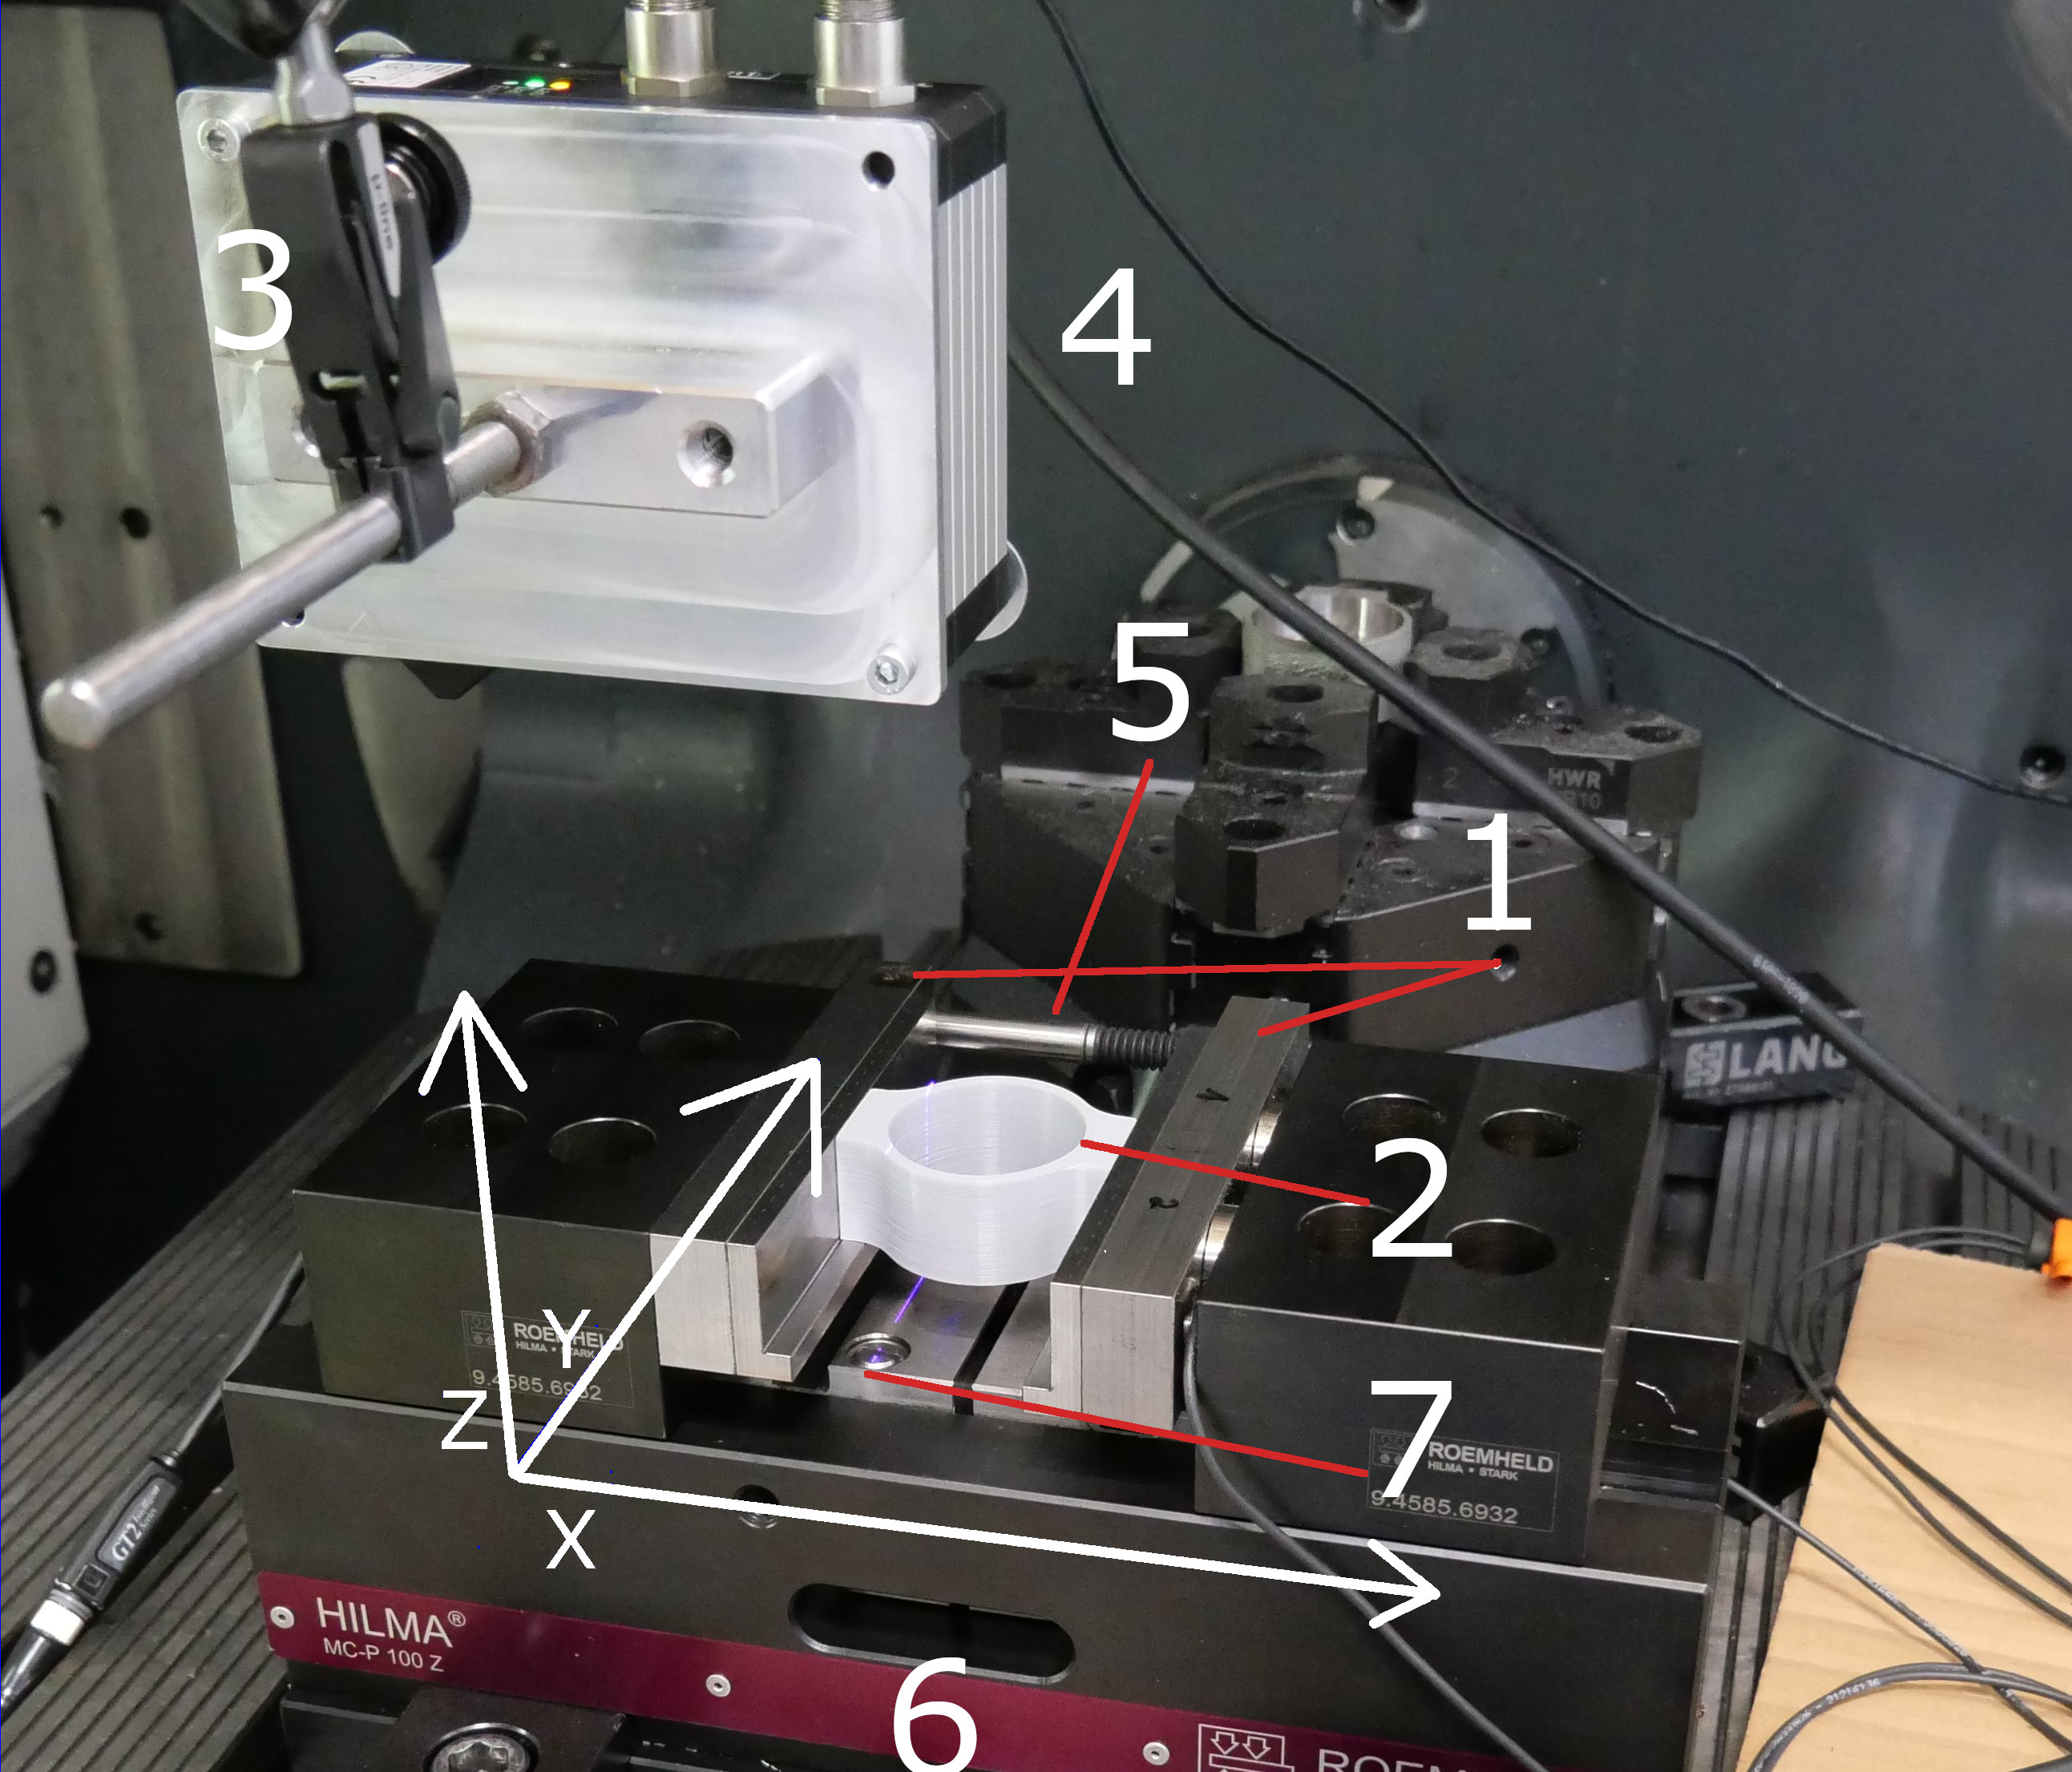
\includegraphics[width=0.6\textwidth]{images/versuchsaufbau_foto.png.JPG}
    \caption{Versuchsaufbau}
    \label{fig:versuchsaufbau}
\end{wrapfigure}

In Abbildung \ref{fig:versuchsaufbau} ist der Versuchsaufbau zur Datenerfassung 
zu sehen. Alle wichtigen Bestandteile sind nummeriert. Es folgt eine kurze Benennung
aller vorhandenen und notwendigen Teile:\\
1: Schraubstock Backen\\
2: Demonstratorbauteil\\
3: Scannerhalterung\\
4: Scanner LLT 30x0-25\\
5: Verschiebungsmesser\\
6: Laserlinie (Lila)\\
7: Schraubstock mit Kraftmesser\\
X: x-Achse\\
Y: y-Achse\\
Z: z-Achse\\

Der Scanner ist an dem Werkzeugkopf einer CNC-Fräse befestigt und wird 
in Richtung der X und Y Achse verschoben. So kann von dem kompletten Bauteil eine 
Pointcloud aufgenommen werden.

\subsubsection{Geschwindigkeit}
Der Parameter `Geschwindigkeit` muss der realen Vorlaufgeschwindigkeit des Scanners
entsprechen um eine korrekte und akkurate Pointcloud zu erhalten. Ist die 
Messgeschwindigkeit kleiner als die Bewegung des Scanners werden Profile doppelt 
aufgenommen, ist sie zu hoch werden Profile übersprungen und das Bauteil wirkt in 
der resultierende Pointcloud in X-Richtung gestreckt.

\begin{wrapfigure}{l}{0.25\textwidth}
    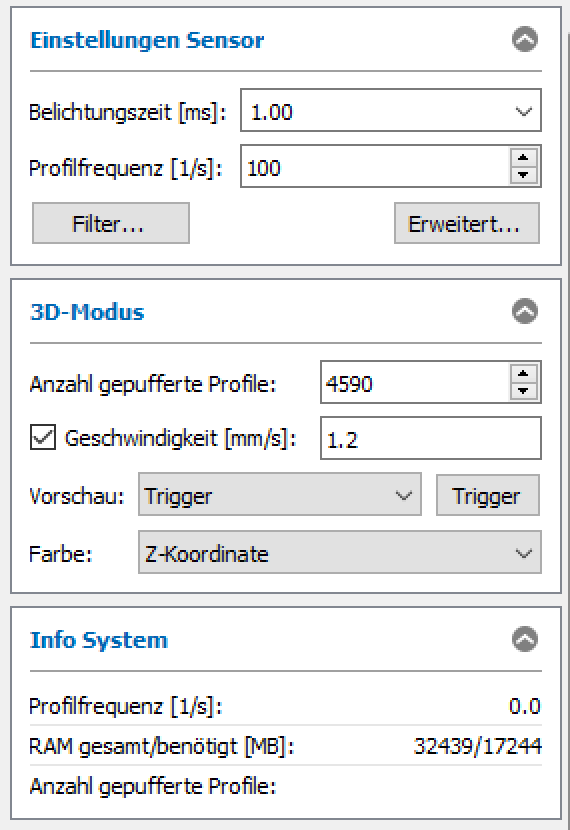
\includegraphics[width=0.25\textwidth]{images/Parameter_Scan.png}
    \caption{Scanparameter}
    \label{fig:scanparameter}
\end{wrapfigure}

\subsubsection{Limitierungen der Achsen:}

Die gesamte Länge des Objekts kann also erfasst werden, indem Scanner 
beziehungsweise Werkzeugkopf in X-Richtung verschoben wird. Mit dem Start der 
Bewegung muss auch die Aufzeichnung der Scannerdaten beginnen. In unserem Fall wurde
die Datenerfassung manuell per Hand im richtigen Zeitpunkt über die Software 
'SCANControl' von micro-epsilon gestartet. 
Eine mögliche Verbesserung ist es, diesen Vorgang zu automatisieren, indem der 
Scanner automatisch mit dem Start der Bewegung getriggert wird und die Aufzeichnung
startet. Die Länge der Aufzeichnung wird auch über die Software eingestellt. 
In Abbildung \ref{fig:scanparameter} sind die korrekten Parameter für das 
Demonstratorbauteil zu sehen. Über den Parameter 'Anzahl gepufferte Profile' kann 
die Länge der Aufzeichnung eingestellt werden. Limitiert wird dieser Parameter 
durch den verfügbaren Speicher auf dem Zielsystem. Es sollte auch darauf geachtet 
werden das der Scanner mindestens genauso lange bewegt wird wie Aufzeichnung läuft, 
ist dies nicht der Fall entsteht eine Pointcloud die einmal größer als notwendig ist, 
und außerdem am Ende der x-Achse nur wiederholende Profile beinhalten. 
Die y-Achse der Pointcloud wird durch den eingesetzten Scanner limitiert. 

\begin{wrapfigure}{r}{0.2\textwidth}
    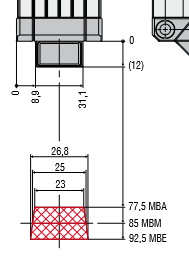
\includegraphics[width=0.2\textwidth]{images/Scanner.PNG}
    \caption{Scanner}
    \label{fig:scanner}
\end{wrapfigure}

Der Scanner hat Abhängig vom Modell und der angebrachten Höhe eine fixe Länge die 
er aufnehmen kann. In unserem Fall wurde der Scanner 'LLT 30x0-25' verwendet der 
eine mittleren Messbreite von 25 mm bietet. 
(Siehe Abbildung \ref{fig:scanner} \cite{MESSTECHNIK_2020}) 
Bauteile mit einer größeren Länge in Y-Richtung können also nicht in einer Pointcloud
erfasst werden. Damit eine Digitalisierung von größeren Objekten erfolgen kann, müssen
also mehrere Scans durchgeführt, und später zusammengefügt werden. Zwischen den 
Scanvorgängen muss der Scanner in Y-Richtung verschoben werden.
Die Länge der Verschiebung sollte 
kleiner als die Scannerbreite sein, damit eine Überlappung entsteht, die 
genutzt werden kann, um die Pointclouds wieder zusammenzufügen. Die Verschiebung kann 
beliebig klein gewählt werden, jedoch steigt der Arbeitsaufwand und die Dateigröße mit 
jeder zusätzlichen Pointcloud, während das Ergebnis sich nicht verbessert.
So können Pointclouds aufgenommen werden die dann in dem zu entwickelnde Verfahren
wieder zu einem digitalen Abbild zusammengefügt werden. Ist dieser Prozess erfolgreich
erhält, man eine Pointcloud der Oberfläche des Objekts. 
In Abbildung \ref{fig:pointcloud_big} ist eine Pointcloud von dem Demonstratorbauteil
zu sehen, in Abbildung \ref{fig:pointcloud_small} eine Nahaufnahme des mittleren Teils
derselben Pointcloud in der die einzelnen Punkte sichtbar sind. Hier sieht man wie
die Pointcloud aufgebaut ist. Dazu aber später noch etwas mehr.

\begin{figure}[h]
    \centering
    \begin{minipage}{0.45\textwidth}
        \centering
        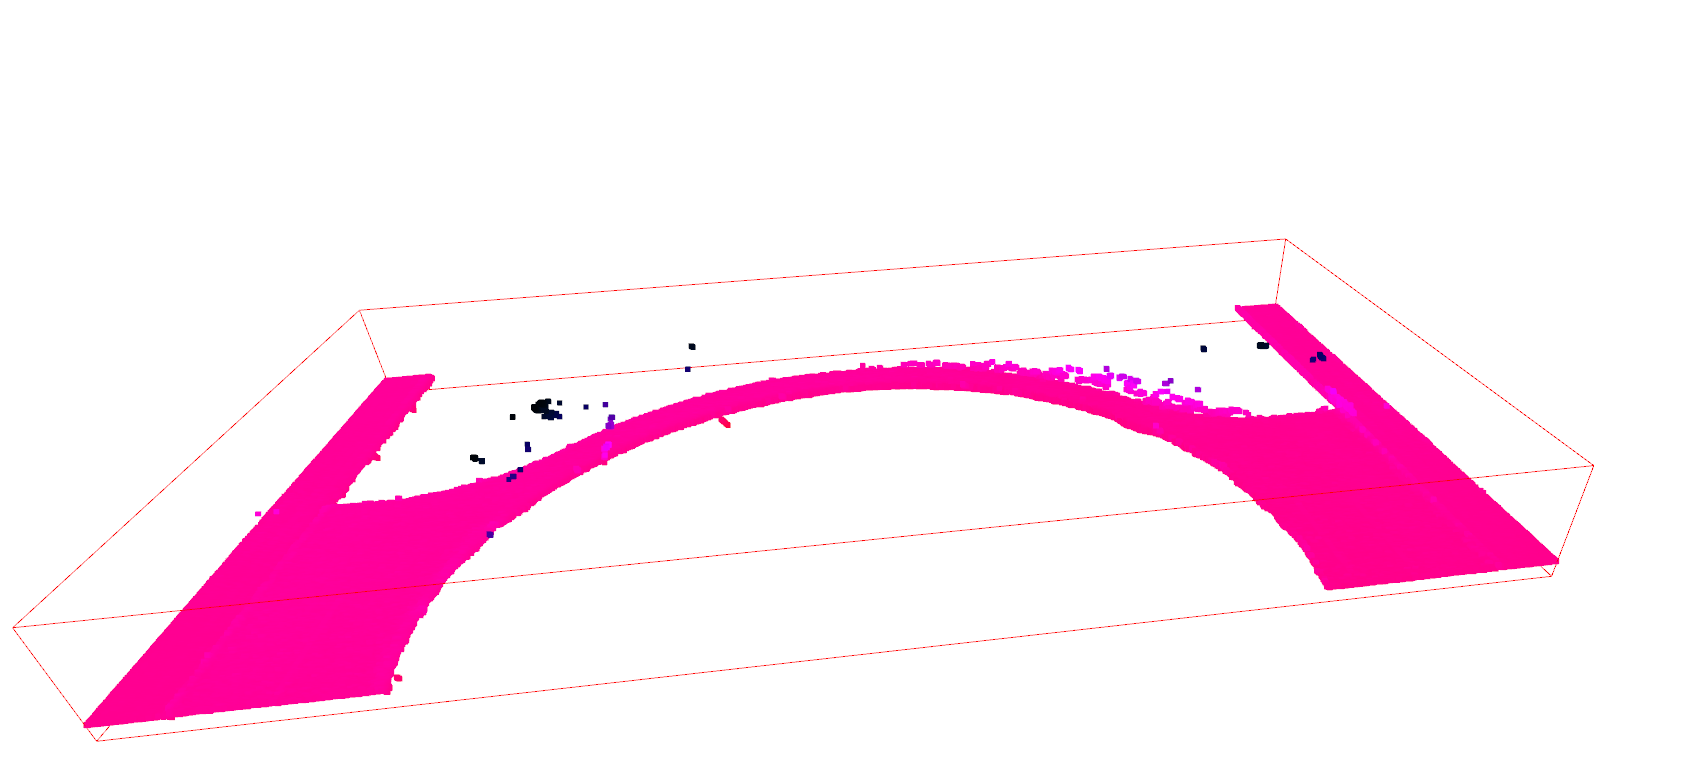
\includegraphics[width=0.9\textwidth]{images/pointcloud_big.PNG} % first figure itself
        \caption{Pointcloud}
        \label{fig:pointcloud_big}
    \end{minipage}\hfill
    \begin{minipage}{0.45\textwidth}
        \centering
        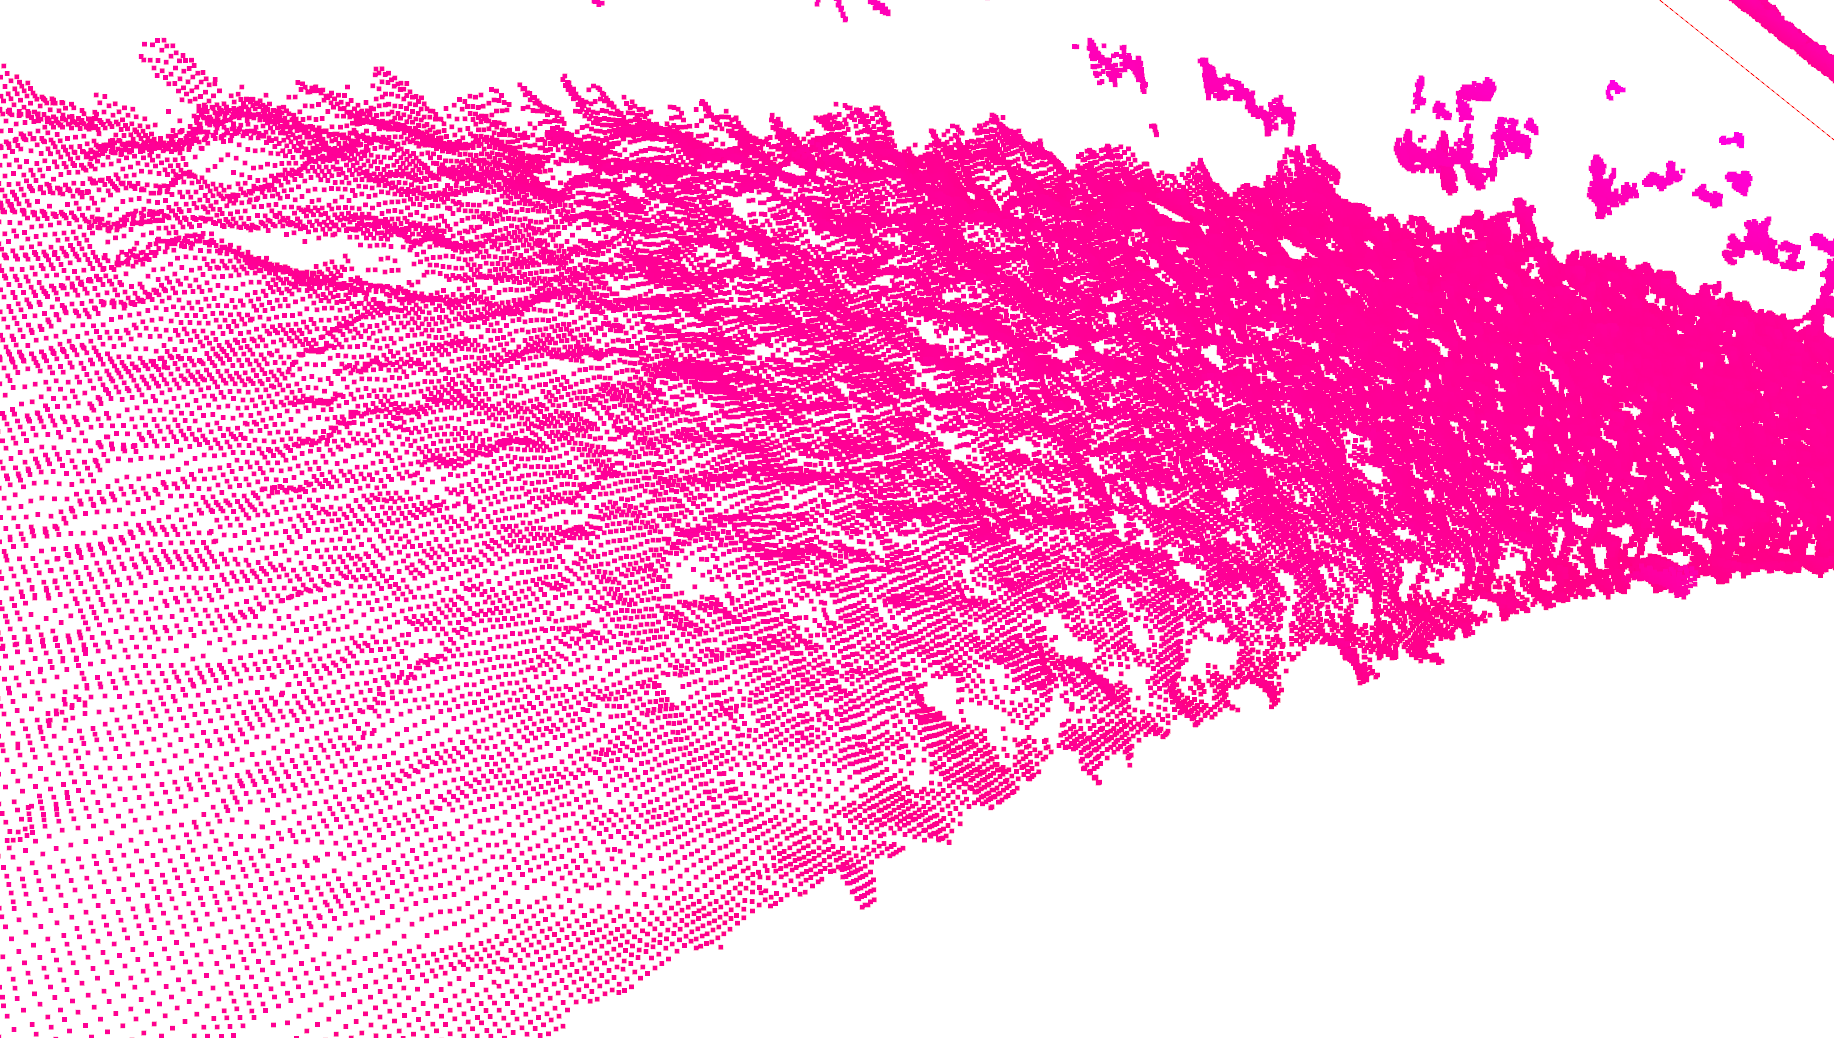
\includegraphics[width=0.9\textwidth]{images/pointcloud_small.PNG} % second figure itself
        \caption{Nahaufnahme Pointcloud}
        \label{fig:pointcloud_small}
    \end{minipage}
\end{figure}

\needspace{0.4\textwidth}
\begin{wrapfigure}{r}{0.4\textwidth}
    \includegraphics[width=0.4\textwidth]{images/taster.JPG}
    \caption{Taster}
    \label{fig:taster}
\end{wrapfigure}

\subsubsection{Zusätzliche Messinstrumente}

Zusätzlich zu dem Scanner werden noch mit weiteren Elementen Daten erfasst.
In Abbildung \ref{fig:versuchsaufbau} unter der Nummer 5 ist ein mechanischer 
Verschiebungsmesser zu sehen. Dieser misst die Verschiebung der Backen des 
Schraubstocks. Der Schraubstock misst zusätzlich mit viel Kraft die Backen 
aufeinander pressen. Damit die Scanner-Ergebnisse überprüft werden können 
wird die Bauteilgeometrie zusätzlich nach dem Scanvorgang noch mit einem Taster
abgetastet. Hierfür wird der Werkzeugkopf gewechselt und der Scanner entfernt.
Dann wird der Taster in die CNC-Maschine eingesetzt und das Bauteil abgetastet.
In Abbildung \ref{fig:taster} ist das Tasterwerkzeug zu sehen. Die rote Kugel 
am Ende des Tasters erkennt, sobald eine Berührung zu dem Bauteil erfolgt ist 
und benachrichtigt den Steuerungsrechner. Dieser speichert die aktuelle Position 
dann in einer Protokolldatei. 

Bevor ich mich aber mit dem 2. Schritt des Verfahrens beschäftigen möchte ich auf die 
Datenstruktur von Pointclouds eingehen. Wie der Name schon sagt bestehende
Pointclouds aus Punkten. In unserem Fall ca. 3 Millionen für eine einzelne
Bewegung in X-Richtung. In jedem Punkt sind mindestens 3 Koordinaten gespeichert, 
eine X und Y Koordinate relativ zu Ursprung der Pointcloud und eine Z Koordinate 
in der die Höhe gespeichert wird. Der Ursprung der Pointcloud liegt in der Mitte 
der x-Achse, also genau da wo der Scanner verläuft.
Zusätzlich ist für jeden Punkt auch noch eine Farbe als RGB-Farbwert
(3 Werte von 0 bis 255) gespeichert. Die Farbe wird relativ zu der Höhe
berechnet. Punkte bekommen einen Farbwert zugewiesen je nachdem wie nah 
sie an dem Minimum oder Maximum der Z-Koordinate sind. 
In \ref{fig:pointclouds} ist die komplette Pointcloud eines Demonstratorbauteils 
zu sehen, zusammen mit einer BoundingBox, durch diese werden die Randpunkte
der Pointcloud visuell dargestellt. Man sieht außerdem das unten liegende Punkte
hell und weiter oben liegende Punkte dunkler dargestellt werden.
Unterhalb ist eine Nahaufnahme des Mittelstücks des gleichen Bauteils zu sehen. 
Hier sind die einzelnen Punkte sichtbar.

Die Koordinaten sind als Float gespeichert haben keinerlei Bezug zueinander.
Das heißt die X und Y Koordinaten sind nicht zum Beispiel anhand eines Netzes
angelegt, sondern können einen beliebigen Abstand zwischen einander haben. Das
werden wir auch später in der weiteren Bearbeitung der Pointclouds sehen.

Wenn nun also alle Pointclouds für ein Objekt erfasst wurden kann zu dem 2.
Schritt des Verfahrens übergegangen werden. Hier müssen die Daten zusammengefügt 
werden. 
Hierfür existieren in der Literatur schon verschiedene Verfahren, ein 
besonders beliebtes ist der ICP-Algorithmus.
Dieser Algorithmus existiert schon seit dem Beginn der 90er Jahre und ist 
die klassische Methode, wenn es um die Registrierung von Pointclouds und 
anderen Punkt-Sets geht. \cite[]{icp}
Der Algorithmus errechnet eine lokale, optimale Transformation die ein Datenset
dem anderen annähern kann. \cite{icp_og}
Um diese Transformation zu bestimmen werden zuerst die Distanzen von allen 
Punkten in Datenset A zu dem jeweils nächsten Punkt in Datenset B aufsummiert 
werden. Dann wird eins der Datensets verschoben und rotiert und wieder die 
Distanzen gebildet. Dies wird so lange gemacht bis die Änderung der Distanzen 
konvergiert. Die entstehende Transformation ist dann optimal.
Für identische Datensets die sich nur in einer Transformation und Rotation 
unterscheiden, funktioniert dieser Algorithmus sehr gut. Bei Datensätzen die 
Messfehler oder Überlappungen beinhalten kann häufig keine optimale 
Transformation bestimmt werden.
Deswegen wurden seit der ersten Vorstellung des Algorithmus viele Varianzen
entwickelt, die mit diesem Schwächen umgehen. 
Zum Beispiel der 'Sparse Iterative Closest Point' Algorithmus von \cite{Bouaziz.2013}
oder die 'Anderson-accelerated' Version die besser mit Ausreißern und nur 
partiell überlappenden Daten umgehen kann und eine gleichwertige oder bessere 
Transformation errechnen kann. \cite{icp}

\begin{wrapfigure}{l}{0.2\textwidth}
    \centering
    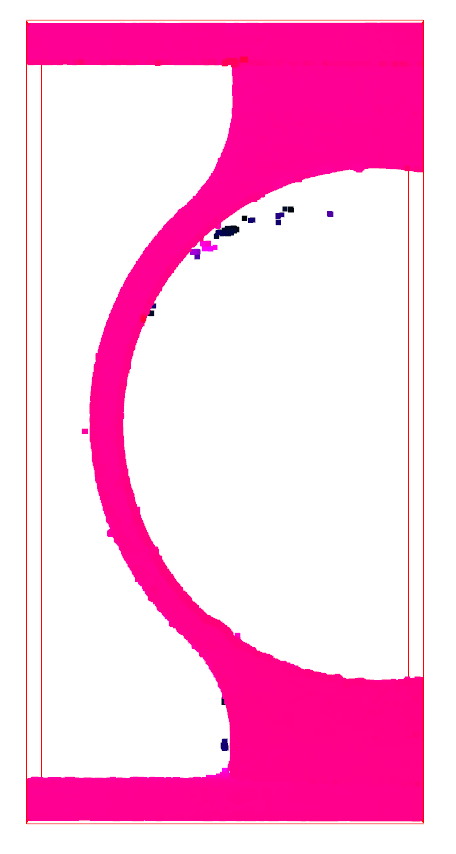
\includegraphics[width=0.2\textwidth]{images/demonstratorbauteil_top.PNG}
    \smallskip\par
    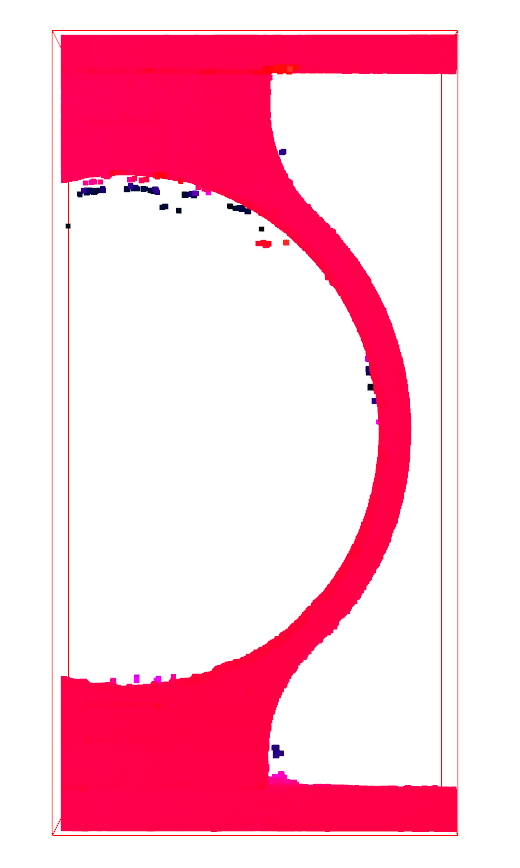
\includegraphics[width=0.2\textwidth]{images/demonstratorbauteil_bottom.PNG}
    \caption{Demonstratorbauteil}
    \label{fig:demonstratorbauteil}
    \vspace{-20pt}
\end{wrapfigure}

Aufgrund der Versprechen dieser Varianten und weil dieser Algorithmus in vielen
Open-Source Bibliotheken schon implementiert ist, war das auch mein erster Ansatz
und ich habe mir Hoffnungen gemacht, dass das Zusammenfügen der Pointclouds 
damit schnell abgehakt ist. 
Dafür habe ich die Methode der Global Registrierung aus der Open3D Bibliothek genutzt
die auf dem Paper von Qian-Yi Zhou, Jaesik Park und Vladlen Koltun basiert. \cite{Zhou.}
Das Globale Registrierung Verfahren wird vor dem ICP-Algorithmus benutzt um eine erste, 
initiale Transformation zu erstellen, die der IPC-Algorithmus im ersten Schritt braucht.

Das Problem bei dieser Methodik und meinem Datensatz ist, das beide Hälften des
Demonstratorbauteils symmetrisch sind. In dem Verfahren wird nicht nur eine Transformation
anhand der X, Y und Z Achsen eingesetzt, sondern auch eine Rotation der Pointcloud.
Wie man in Abbildung \ref{fig:demonstratorbauteil} sehen kann überlappen die beiden Pointclouds 
schon fast zu 100 Prozent, wenn eine Pointcloud um 180 Grad gedreht, und über die andere
gelegt wird. Auf dieses Ergebnis ist auch das Global Registrierungsverfahren gekommen. 
Für unseren Fall ist also ein Verfahren nötig was ausschließlich eine 
Transformation in X und Y Richtung benutzt. Das sind auch die einzigen Achsen, 
in der sich der Scanner bewegt hat.

\subsection*{Wahl des Demonstratorbauteils}

Man könnte sich jetzt hier die Frage stellen, warum das Demonstratorbauteil dann so gewählt 
und entworfen wurde das es symmetrisch ist. In dem ersten Schritt des zusammenfügen ist 
die Bauteilgeometrie zwar hinderlich, dafür profitiert die 
Spannkraftdeformationserkennung von dem initial runden Innenkreis des Bauteils.
Zusätzlich soll das hier zu entwickelnden Verfahren auf viele Bauteilgeometrien 
anwendbar sein und somit nicht durch eine Symmetrie beschränkt werden.

\subsection*{Weitere Verfahren}

Nachdem die globale Registrierung und der ICP-Algorithmus auf den Pointclouds nicht
anwendbar waren musste ein anderes Verfahren her. Aufgrund weniger schon existieren 
Verfahren die eine reine Bewegung auf nur 2 Achsen verwenden habe ich eine Idee 
entworfen, die auf dem ICP-Algorithmus basiert, um 2 Pointclouds zu vergleichen 
und zu verschieben. Hierfür habe ich die Pointclouds in ein zweidimensionales Array
mit den Z-Werten als Inhalt konvertiert. Nun kann die euklidische Distanz der Z-Werte
und jedem X und Y Wert aufsummiert werden. In einem naiven Ansatz kann dann eine 
Pointcloud entlang der Länge und Breite der anderen Pointcloud bewegt werden und für 
jede Transformation die Summe der Distanzen gespeichert werden. Die Idee war das die 
Transformation mit der kleinsten Summe die beste Überlappungen der beiden Pointclouds 
ist. Das hat aber nicht funktioniert. Durch die tatsächliche relativ kleine Überlappung 
ist die Summe der Distanzen nicht bei der korrekten Transformation minimal, 
sondern, wenn die Pointclouds maximal übereinander geschoben sind. Zusätzlich war die 
Verschiebung und Berechnung der zweidimensionalen Arrays rechenintensiv und hat zu 
langen Laufzeiten geführt. Also habe ich dieses Verfahren wieder aufgeben mit einer neuen
Idee:

\subsection*{Pointcloud in Bild konvertieren}
Um Rechenzeit zu sparen und auf viele Funktionen von schon bestehenden 
Bilderkennungs-Bibliotheken zurückgreifen zu können habe ich die Pointclouds in ein
Bild konvertiert. Hierfür wird zuerst in leeres Bild mit den gleichen Maßen einer 
Pointcloud erstellt. Dann wird über alle Punkte der Pointcloud iteriert und jeweils
der Pixel an der X und Y Koordinate des Punktes auf einen Helligkeitswert gesetzt.
Um Rechenzeit und Speicherkapazitäten zu schonen, und weil es für die Berechnung 
ausreichend ist, habe ich mich für 8 Bit Single-Channel Bilder die nur Helligkeitswerte 
abbilden entschieden. Hier kann also jede Pixel einen Wert zwischen 0 und 255 annehmen.
Der entsprechende Wert kann wie folgt berechnet werden:

\begin{wrapfigure}{r}{0.5\textwidth}
    \centering
    $value_p = \frac{Z - min_y}{max_y - min_y} \cdot (max_b - min_b) + min_b$
    \caption{Berechnung Pixelwert}
    \label{calc:brightness}
\end{wrapfigure}
Der resultierende Wert ist die Helligkeit, die dem Pixel zugewiesen wird.
$Z$ ist die Z-Koordinate des Punktes in der Pointcloud. $min_y$ und $max_y$ sind 
die Grenzen der Z-Koordinate, diese werden gebraucht um die Helligkeit relativ 
zu der Höhe zu berechnen. $min_b$ und $max_b$ sind die gewünschten Grenzen der 
Helligkeit. In unserem Fall sind $min_b = 0$ und $max_b = 255$ da ein 8 Bit Bild
verwendet wird.

\begin{wrapfigure}{l}{0.5\textwidth}
    \centering
    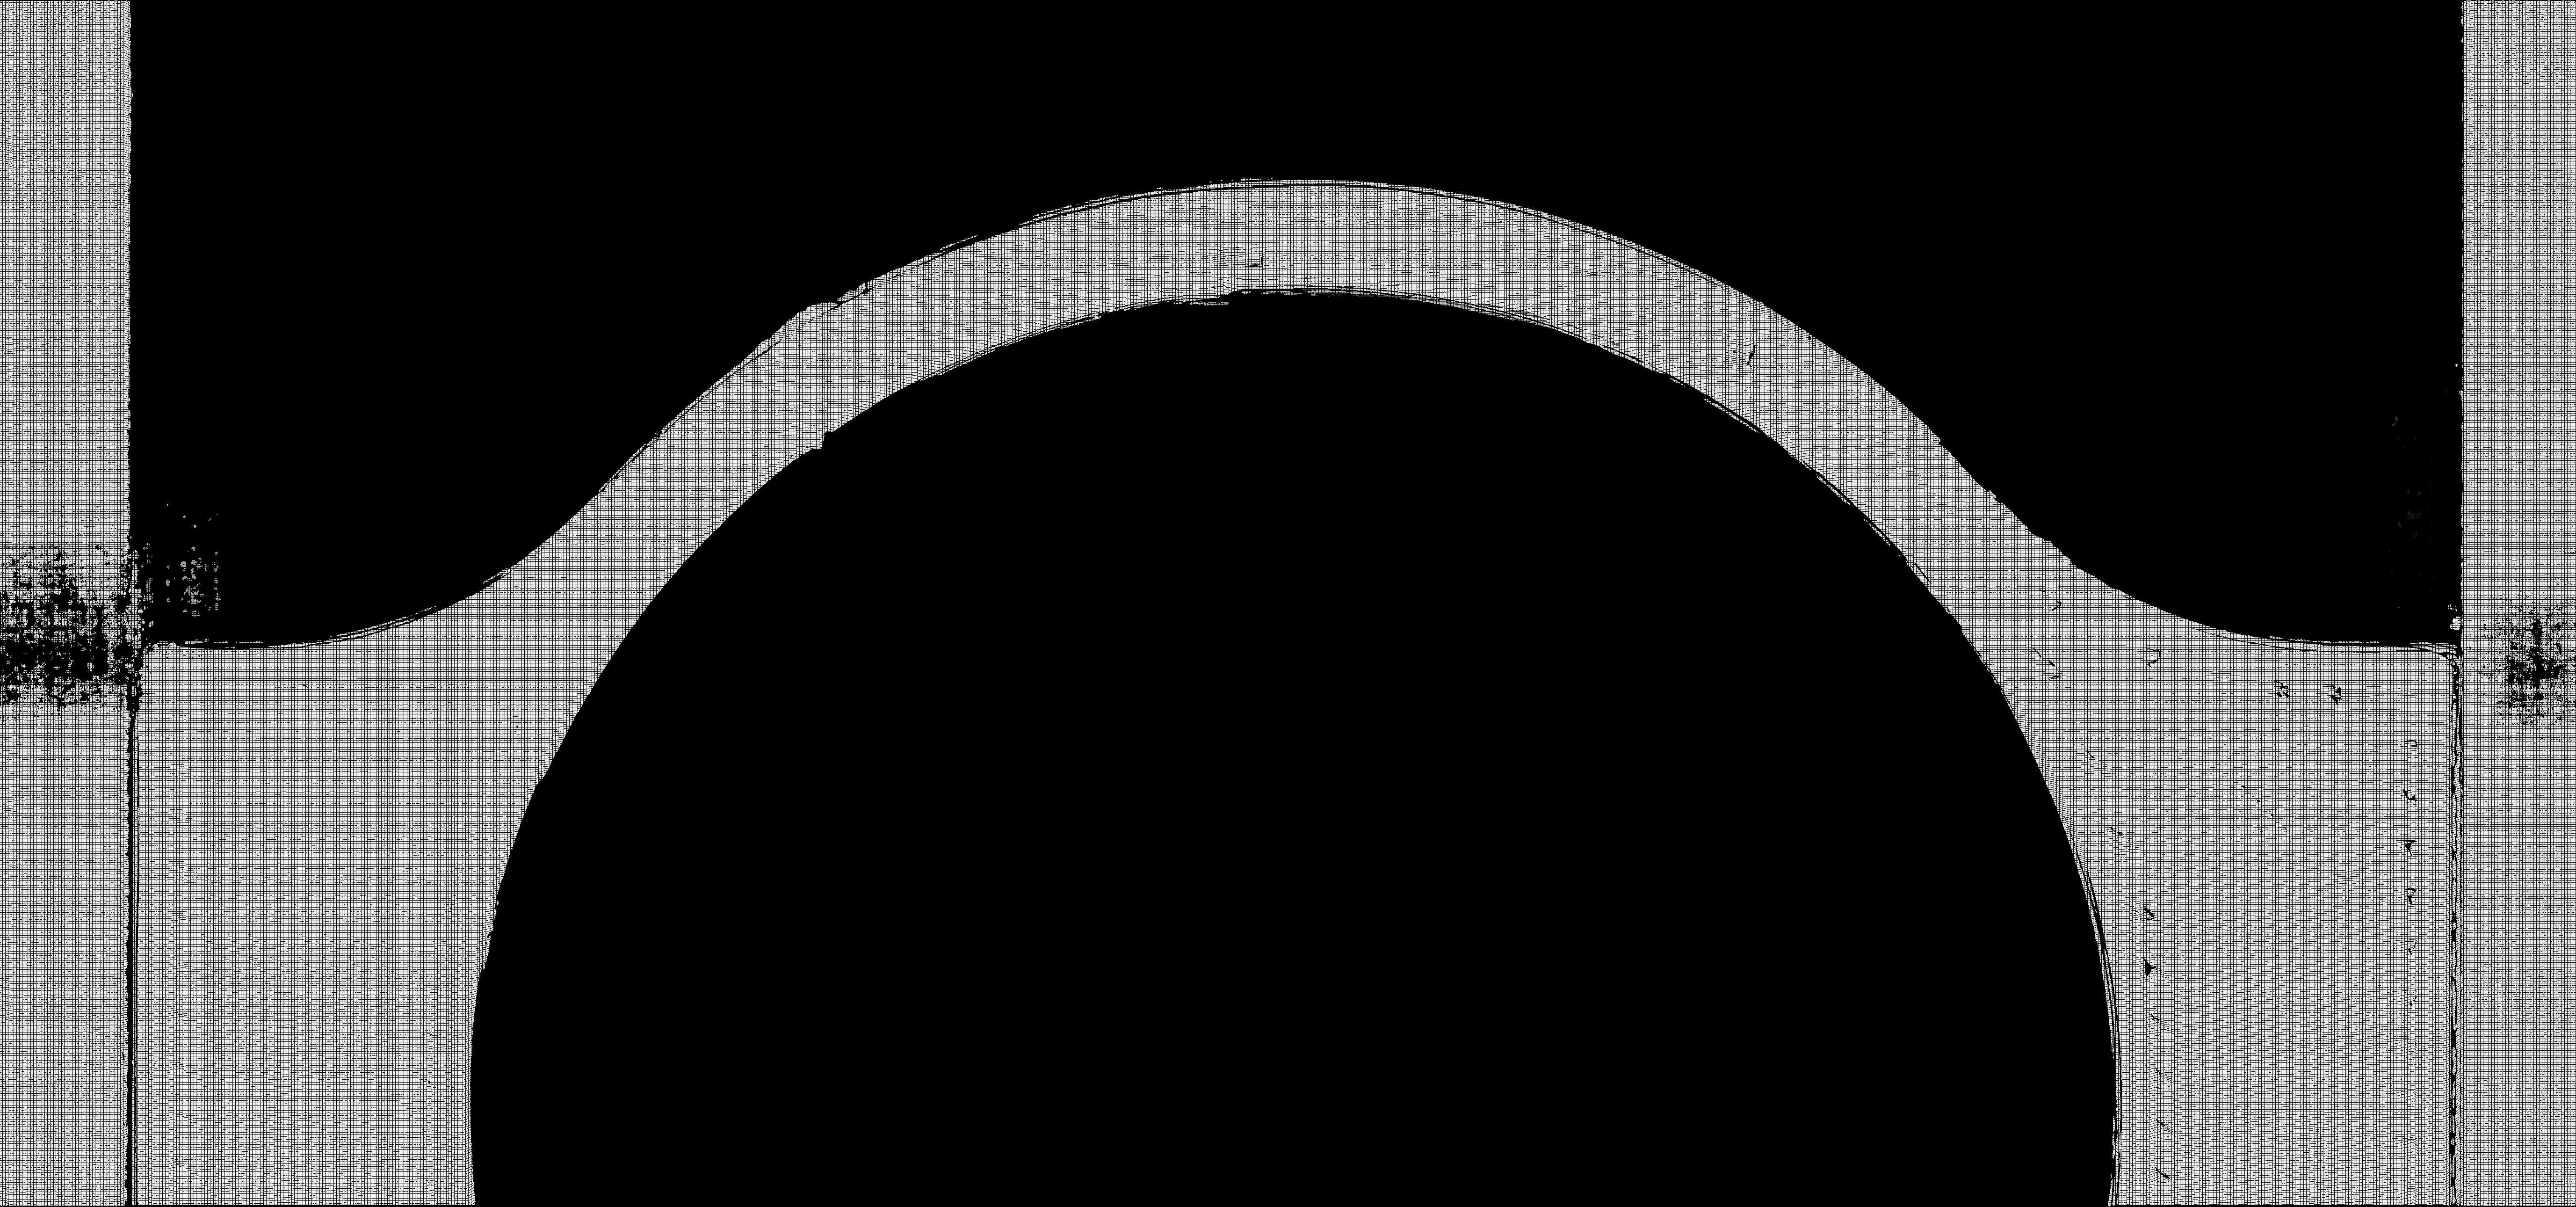
\includegraphics[width=0.5\textwidth]{images/fdm_top_100p.png}
    \includegraphics[width=0.5\textwidth]{images/fdm_top_10p.png}
    \caption{Konvertierung Pointcloud zu Bild}
    \label{fig:image_from_pc}
\end{wrapfigure}

Wie man in Abbildung \ref{fig:image_from_pc} sehen kann, sind kaum Helligkeitsveränderungen
im Bild sichtbar. Das liegt an derselben Problematik, an der der ICP-Algorithmus häufig
scheitert. Reale Datensets wie wir es vorliegen haben sind nicht perfekt, sondern
beinhalten Messfehler und Streuungen. 

Abbildung \ref*{fig:brightness} zeigt die Häufigkeit der gleichen Höhenwerte einer
Pointcloud von dem Demonstratorbauteil als FDM-Druck.
 Auf der y-Achse die relative Häufigkeit.
Die meisten Höhenwerte sind um die 80, sie gehören zu den Punkten, die auf dem 
Demonstratorbauteil liegen, es treten allerdings auch Werte darunter und darüber auf. 
Die in Abbildung \ref*{calc:brightness} vorgestellte Formel benutzt allerdings 
das absolute Minimum und Maximum Werte, 
die Punkte auf dem Bauteil werden also entsprechend wenig
berücksichtigt. Dem kann Abhilfe geschaffen werden, indem Werte, die weniger häufig 
auftreten entfernt werden. Sortiert man alle Höhenwerte nach der Häufigkeit ihres 
auftreten in der Pointcloud und entfernt den n-ten Prozentsatz können Ausreißer 
entfernt werden. Wenn nur die häufigsten 10 Prozent übernommen werden erhält man 
das untere Bild in Abbildung \ref{fig:image_from_pc}

Features auf dem Bauteil können jetzt deutlich besser erkannt werden. Auch zu sehen
sind jetzt die Markierungen auf der linken und Rechten Seite die bei der Registrierung
helfen sollen. Auch schön zu sehen sind die Spuren und Lücken die durch den FDM 
Herstellungsprozess entstehen.

Durch das Filtern der Höheninformationen sind Oberflächenstrukturen nicht nur besser
erkennbar, auch die Ränder treten genauer hervor. Das ist sehr wichtig für das korrekte
zusammenfügen.

Doch wo soll die Grenze gezogen werden, um die Oberfläche möglichst genau zu erkennen,
aber nicht zu viele Höheninformation zu verlieren.

\subsection{Pointcloud filtern}

\begin{wrapfigure}{r}{0.5\textwidth}
    \centering
    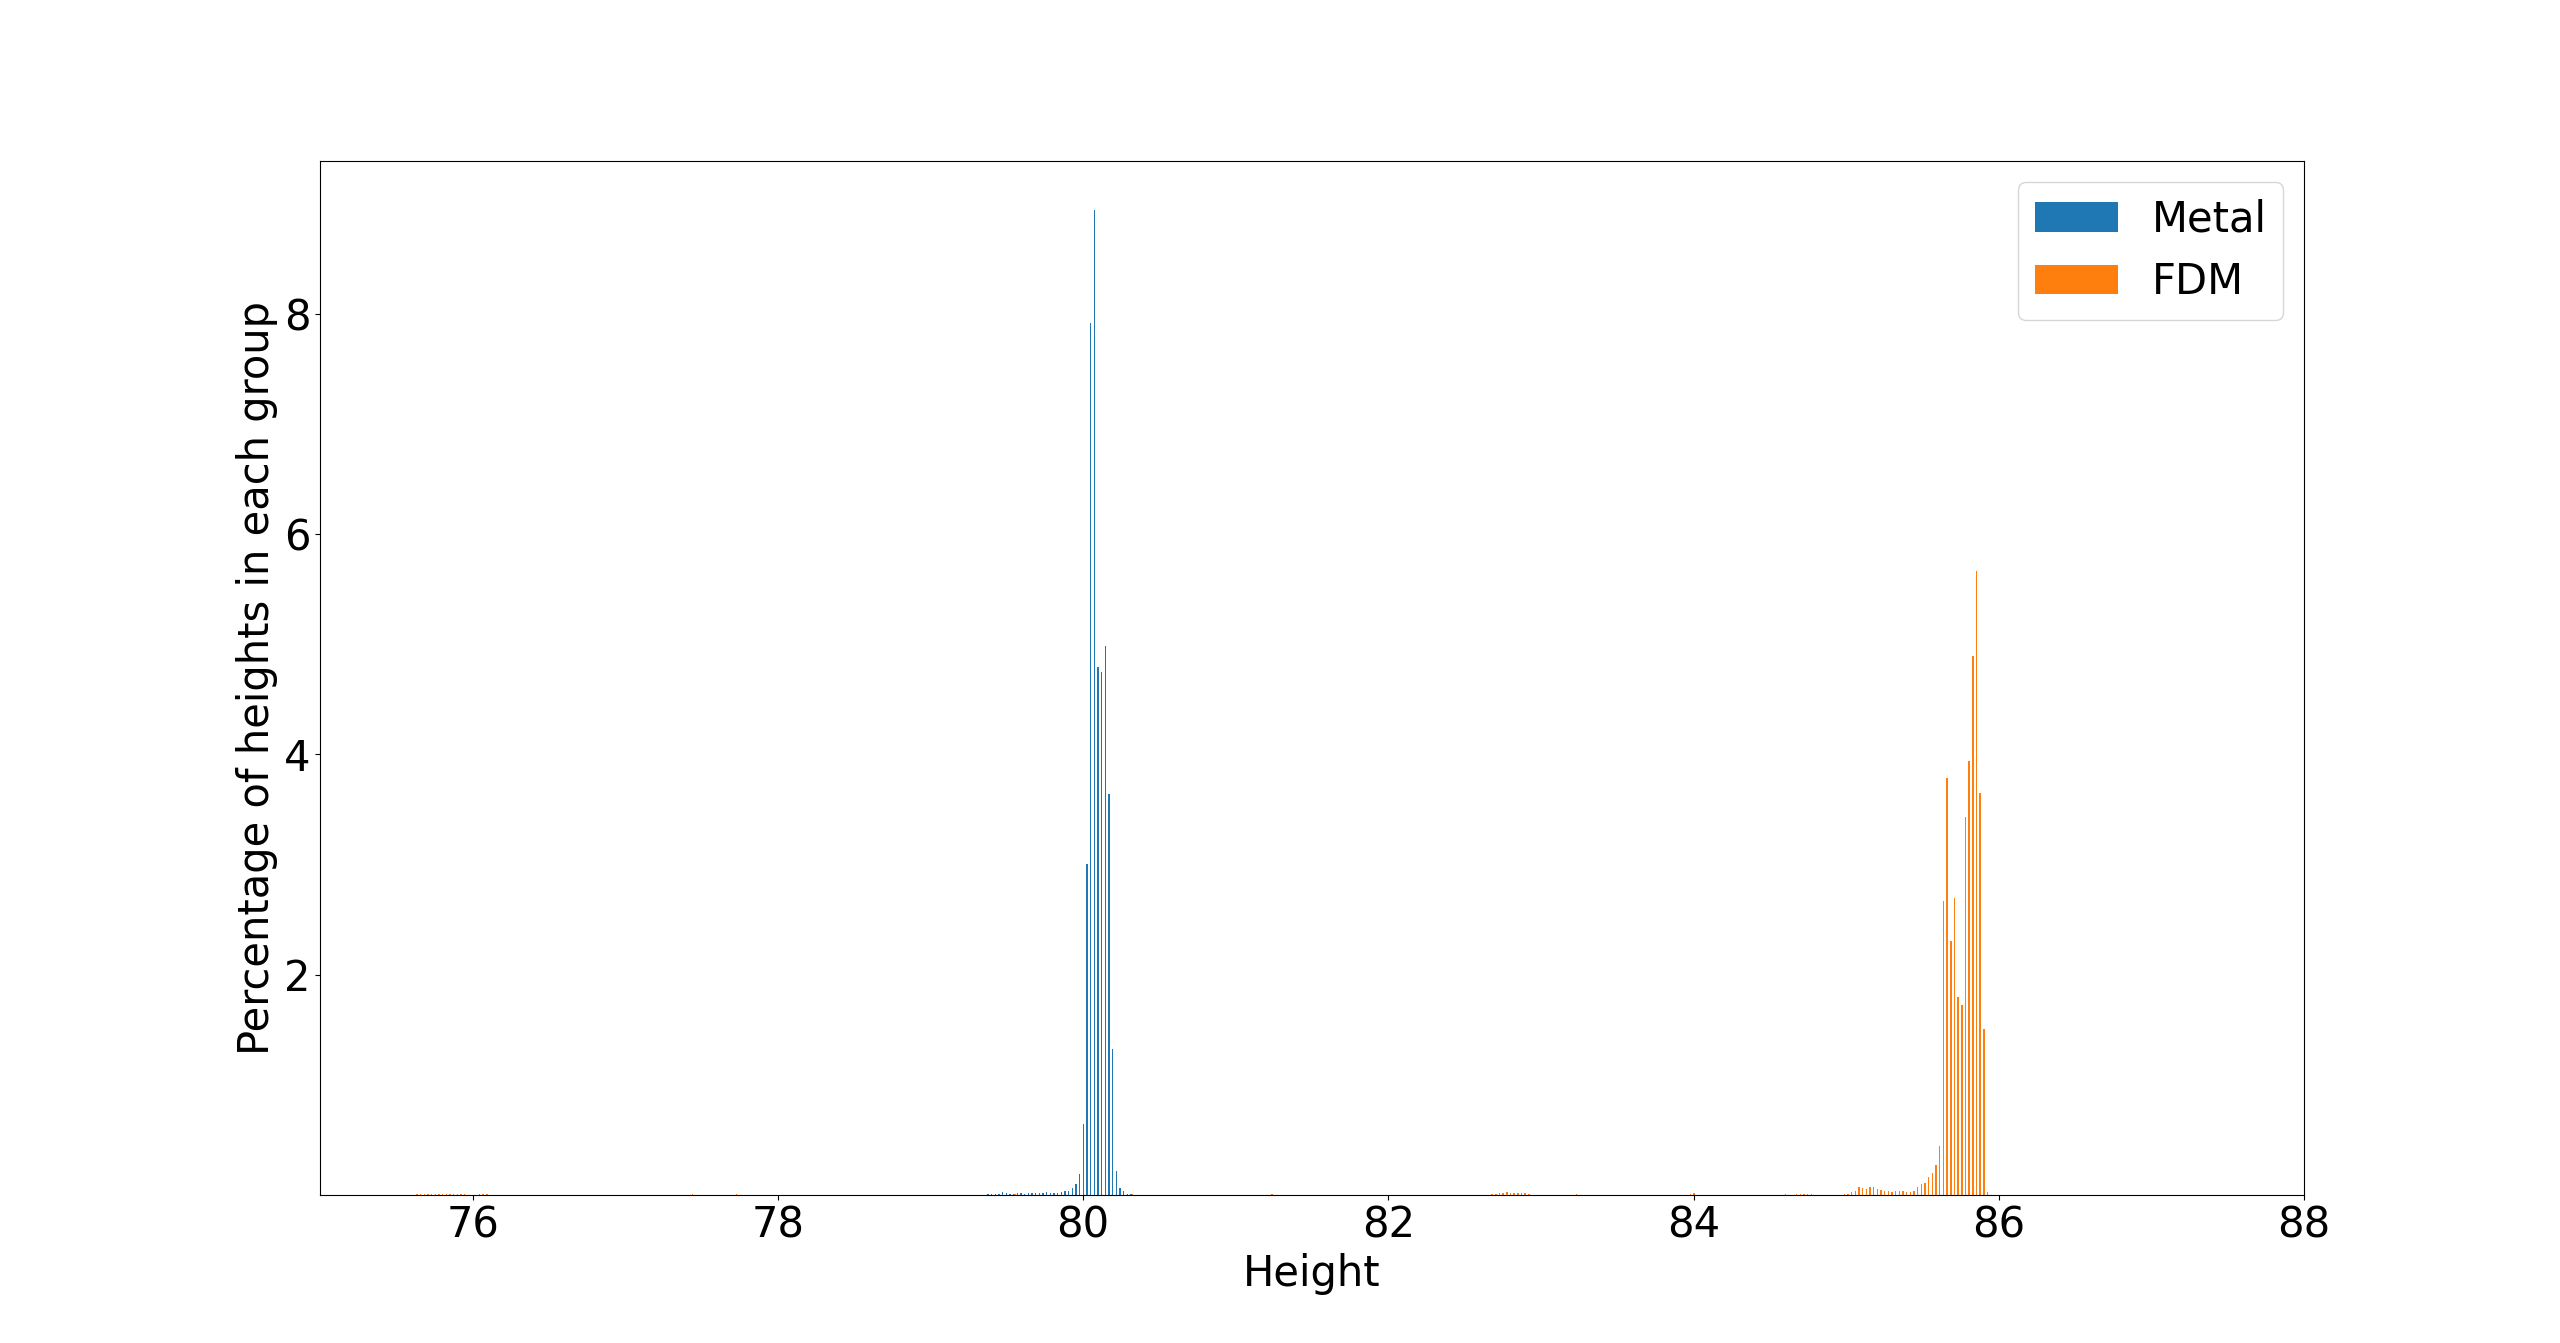
\includegraphics[width=0.5\textwidth]{images/height_occurange.png}
    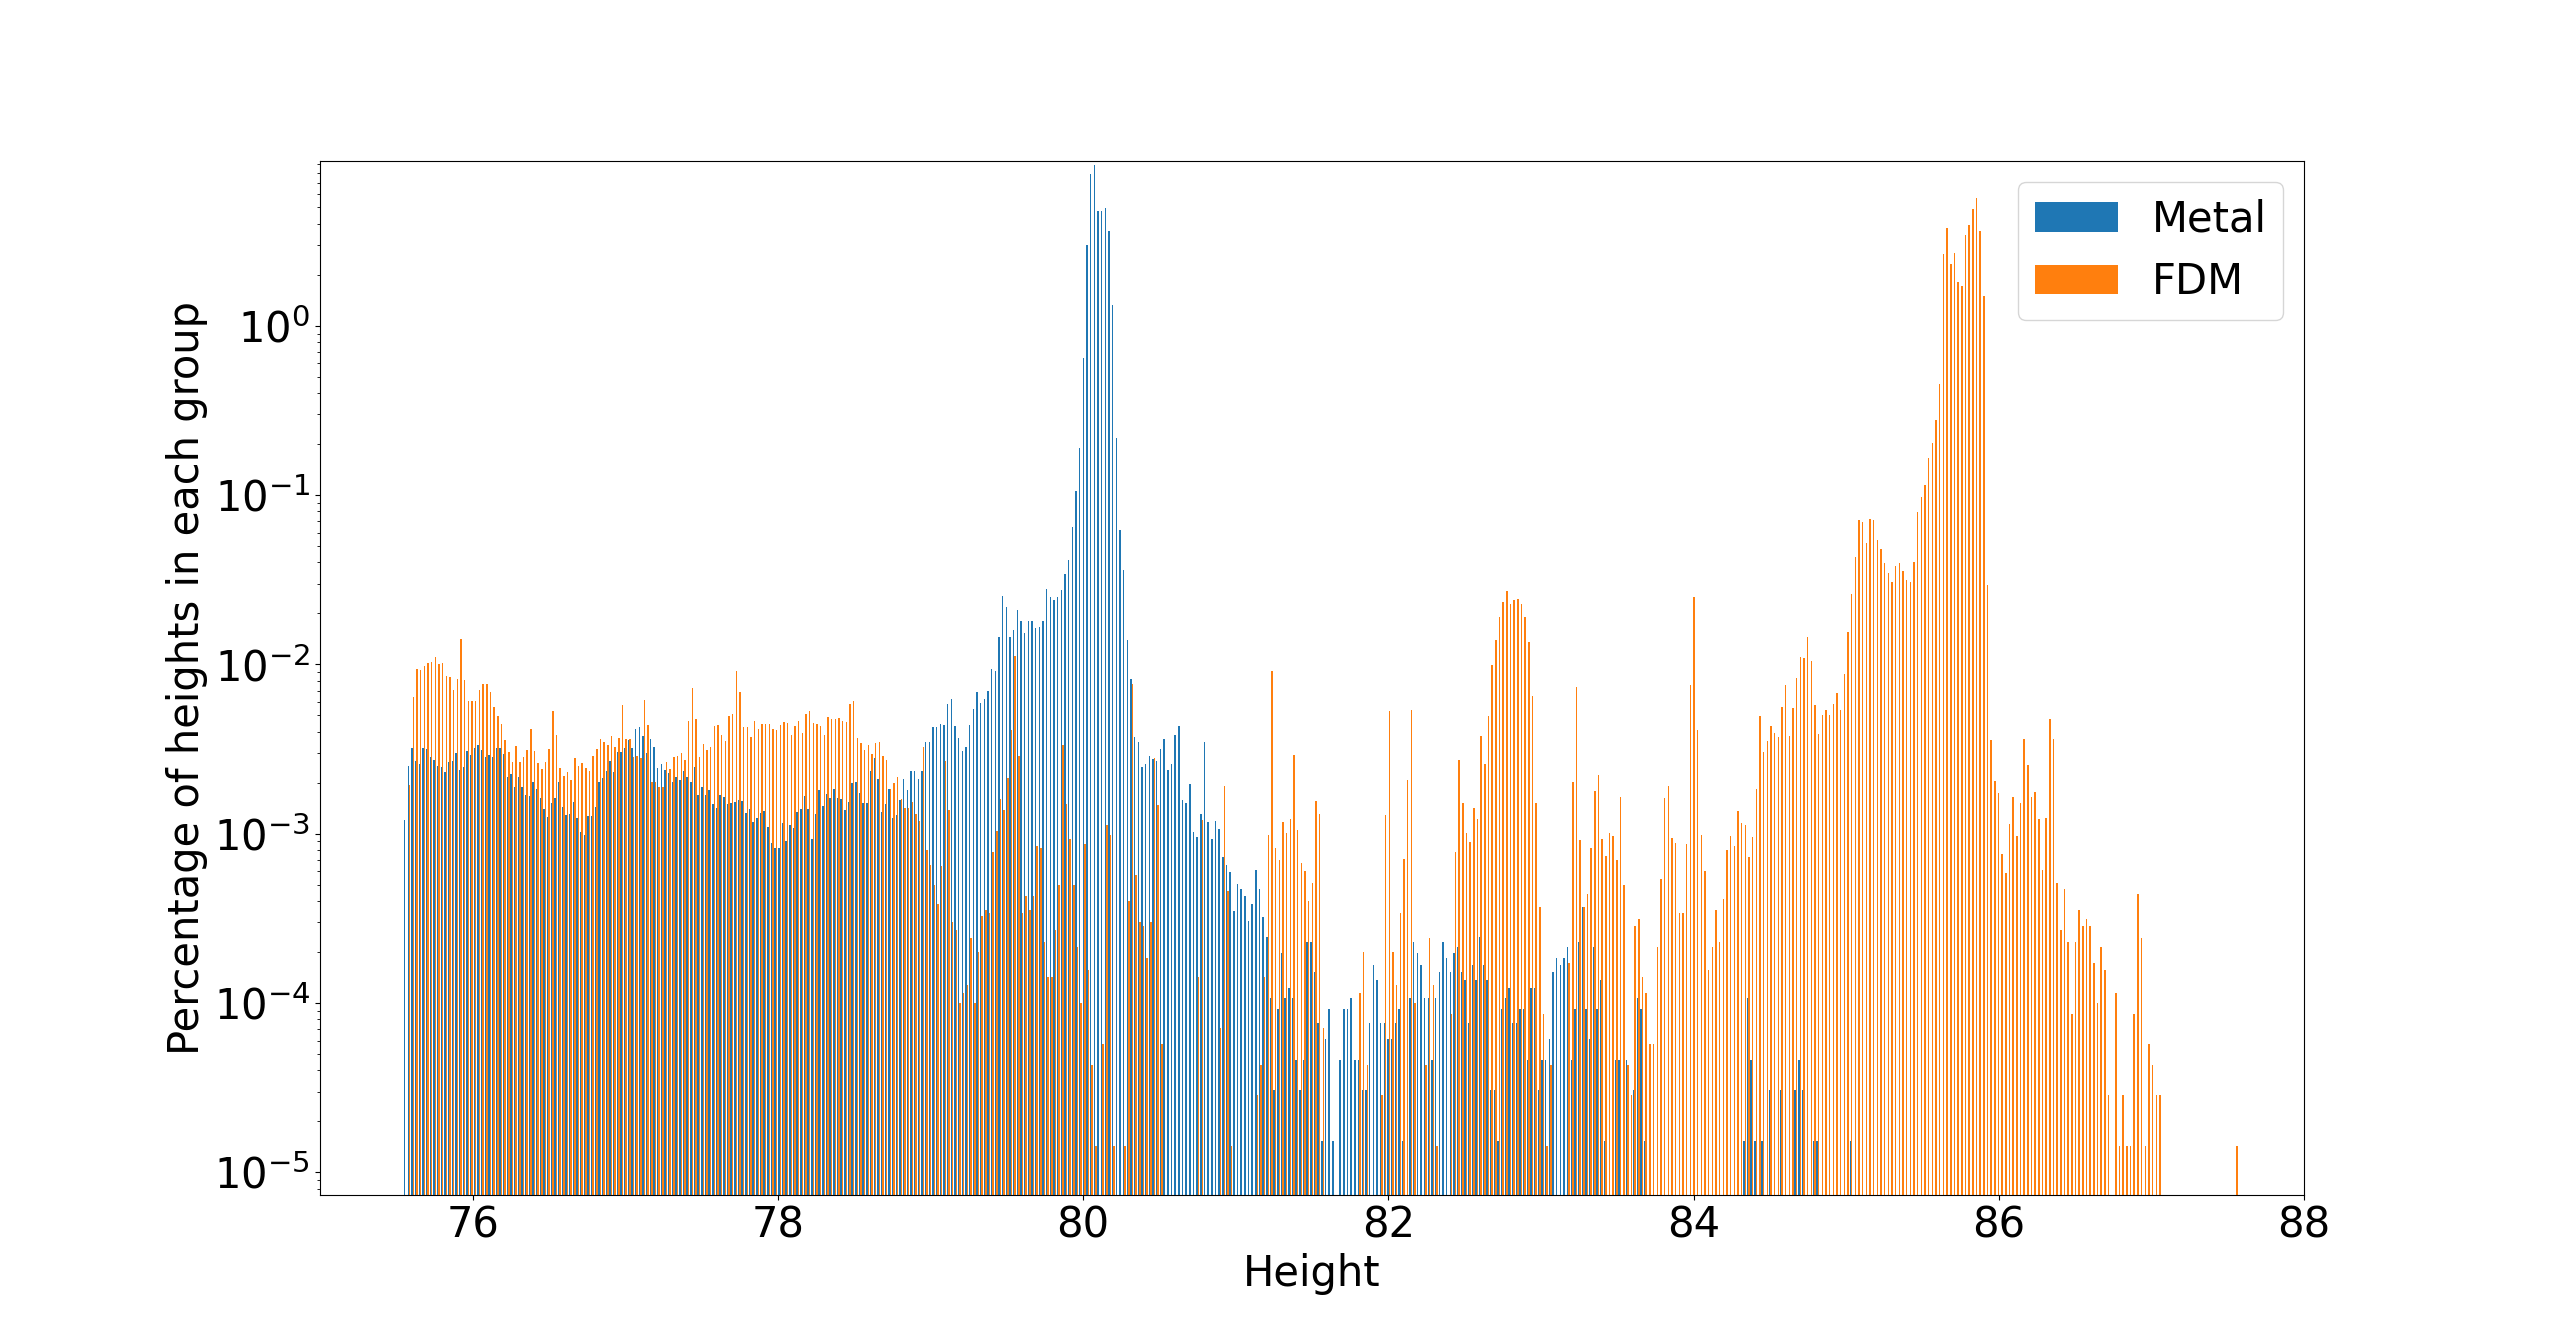
\includegraphics[width=0.5\textwidth]{images/height_occurange_log.png}
    \caption{Auftreten Höhe}
    \label{fig:brightness}
\end{wrapfigure}

Ziel ist das entwickelte Verfahren bei allen gängigen Additiven Fertigungsmethoden
angewendet werden kann, das muss bei der Filterung der Daten berücksichtigt werden
da die Datenverteilung von FDM Bauteilen anders aussieht als bei Metallenen Werkstoffen.
Wie man in Abbildung \ref{fig:brightness} sehen kann streuen nicht alle Pointclouds 
gleich, abhängig von dem Werkstoff des Bauteils werden die Laserstrahlen unterschiedlich
reflektiert und mehr oder weniger Ausreißer sind zu sehen. In dem oberen Histogramm 
sind die Häufigkeiten der Höhenwerte zu sehen, alle Punkte sind in 500 Teile gruppiert.
Unterhalb ist das Histogramm mit dem gleichen Datensatz, aber mit der y-Achse 
logarithmisch
skaliert um kleine Prozente deutlich zu machen die im oberen Diagramm nur schwer oder 
gar nicht sichtbar sind. Man sieht das Metallteil deutlich mehr in beide Richtungen 
streut, während das FDM gedruckte Bauteil weniger nach oben, aber mehr nach unten 
streut. Es muss also eine Filtermethode gewählt werden die für alle Fertigungsverfahren
anwendbar ist und nicht bei einer Methode besser funktioniert wie bei einer 
anderen. Werden zum Beispiel die 10 Prozent häufigst aufkommenden Höhenwerte bei einem
Metallteil benutzt kommt folgendes Bild heraus.

\begin{wrapfigure}{l}{0.4\textwidth}
    \centering
    \includegraphics[width=0.4\textwidth]{images/am_sp0_top_10p.png}
    \caption{Metallteil gefiltert}\label{fig:metall_image}
\end{wrapfigure}

Man sieht vor allem auf der rechten Seite, dass Ränder nicht mehr klar erkennbar sind, 
da sie durch die Filterung Lücken aufweisen. Praxistest haben gezeigt das ein 
ausreichend gut funktionierender Filterwert 50 Prozent ist. Damit werden genug 
Messfehler aus dem Bild genommen aber trotzdem bleiben Oberflächenfeatures und Ränder
sichtbar genug um ein korrektes Zusammenfügen zu gewährleisten.
Dieses Filtern bezieht sich aber nur auf 2 dimensionale Bildinformationen.
Um bei dem Konvertieren noch weniger Punkte die nicht auf dem Bauteil liegen nicht in das Bild zu übernehmen, kann auch noch die Pointcloud gefiltert werden.
Hier kann ein einzelner Punkt relativ zu seinem Nachbarn im 3 dimensionalen Raum betrachtet werden, 
um so Ausreißer zu erkennen. Dafür sind in der Open-Source
Bibliothek 'Open3D' 2 Methoden vorhanden: Radius basiert oder auf Basis von 
statistischen Werten, erste Methode eignet sich gut, wenn die Maße des Objekts bekannt
sind. Hier wird um jeden Punkt eine Kugel gebildet und die Punkte die weniger als 
einen konfigurierbare Menge an Punkte in ihrer Kugel haben werden entfernt. Da 
das hier zu entwickelnde Verfahren sich nicht auf eine Bauteilgeometrie beschränken
ist dieses Verfahren nicht geeignet. Stattdessen wird das andere benutzt. Hier werden
die Punkte entfernt die weiter von ihren benachbarten Punkten entfernt sind als der 
durchschnittliche Abstand der Punkte in der gesamten Pointcloud. Hier kann die Menge der 
benachbarten Punkte die betrachtet werden sollen und ein Limit für den Abstand von der 
Standardabweichung. Umso mehr benachbarte Punkte betrachtet werden, umso mehr Zeit 
braucht die Filterung, aber die Filterung wird auch akkurater. Im Praxistest haben sich
hier 50 Nachbarpunkte bewährt. Mit diesem Wert werden bei Pointclouds in unserem 
Datensatz jeweils ca. 2 Prozent der Punkte entfernt. So kann das resultierende
Bild gut genug umgewandelt werden, um eine erfolgreiche Zusammenführung 
von verschiedenen Bildern zu gewährleisten.
Ein Nachteil bei der Filterung in Abbildung \ref{fig:image_from_pc} links und rechts 
mittig zu sehen. Hier sind schwarze Punkte sichtbar. Diese treten auf, weil der Scanner
hier über dem Bauteil Punkte erkannt hat. Durch das Filtern wurden diese Punkte entfernt
beziehungsweise bei der Konvertierung nicht berücksichtigt. Da diese Punkte dann fehlen
bleiben sie im resultierenden Bild schwarz. Das ist zwar etwas unschön anzuschauen, 
beeinträchtigt das zusammenfügen aber nicht weiter. 

\end{document}

%\newpage

\documentclass[../main.tex]{subfiles}
\begin{document}

\section{Ausgangssituation}

Um die Deformation im eingespannten Zustand zu erkennen, muss das komplette Werkstück
als dreidimensionales Modell existieren. Nur so kann es mit einem anderen Modell 
verglichen werden.

Das Verfahren soll die Deformation nur in einer zweidimensionalen Ansicht erkennen. 
Das ist weniger komplex, hat aber zur Folge, dass Bauteile mit unterschiedlichen 
Oberflächenhöhen nicht korrekt analysiert werden können. 
Die Daten des eingespannten Bauteils liegen inform von mehreren Pointclouds vor.
Diese Daten wurden mithilfe eines Laserscanners aufgenommen. Durch diesen Prozess 
entstehen Messfehler und Ausreißer. Diese Punkte verfälschen das Verfahren da sie 
nicht auf dem eingespannte Bauteil liegen. Die Akkuranz des Verfahrens profitiert, 
wenn diese Punkte entfernt werden.

\subsection{Pointcloud filtern}

\begin{figure}[h]
    \centering
    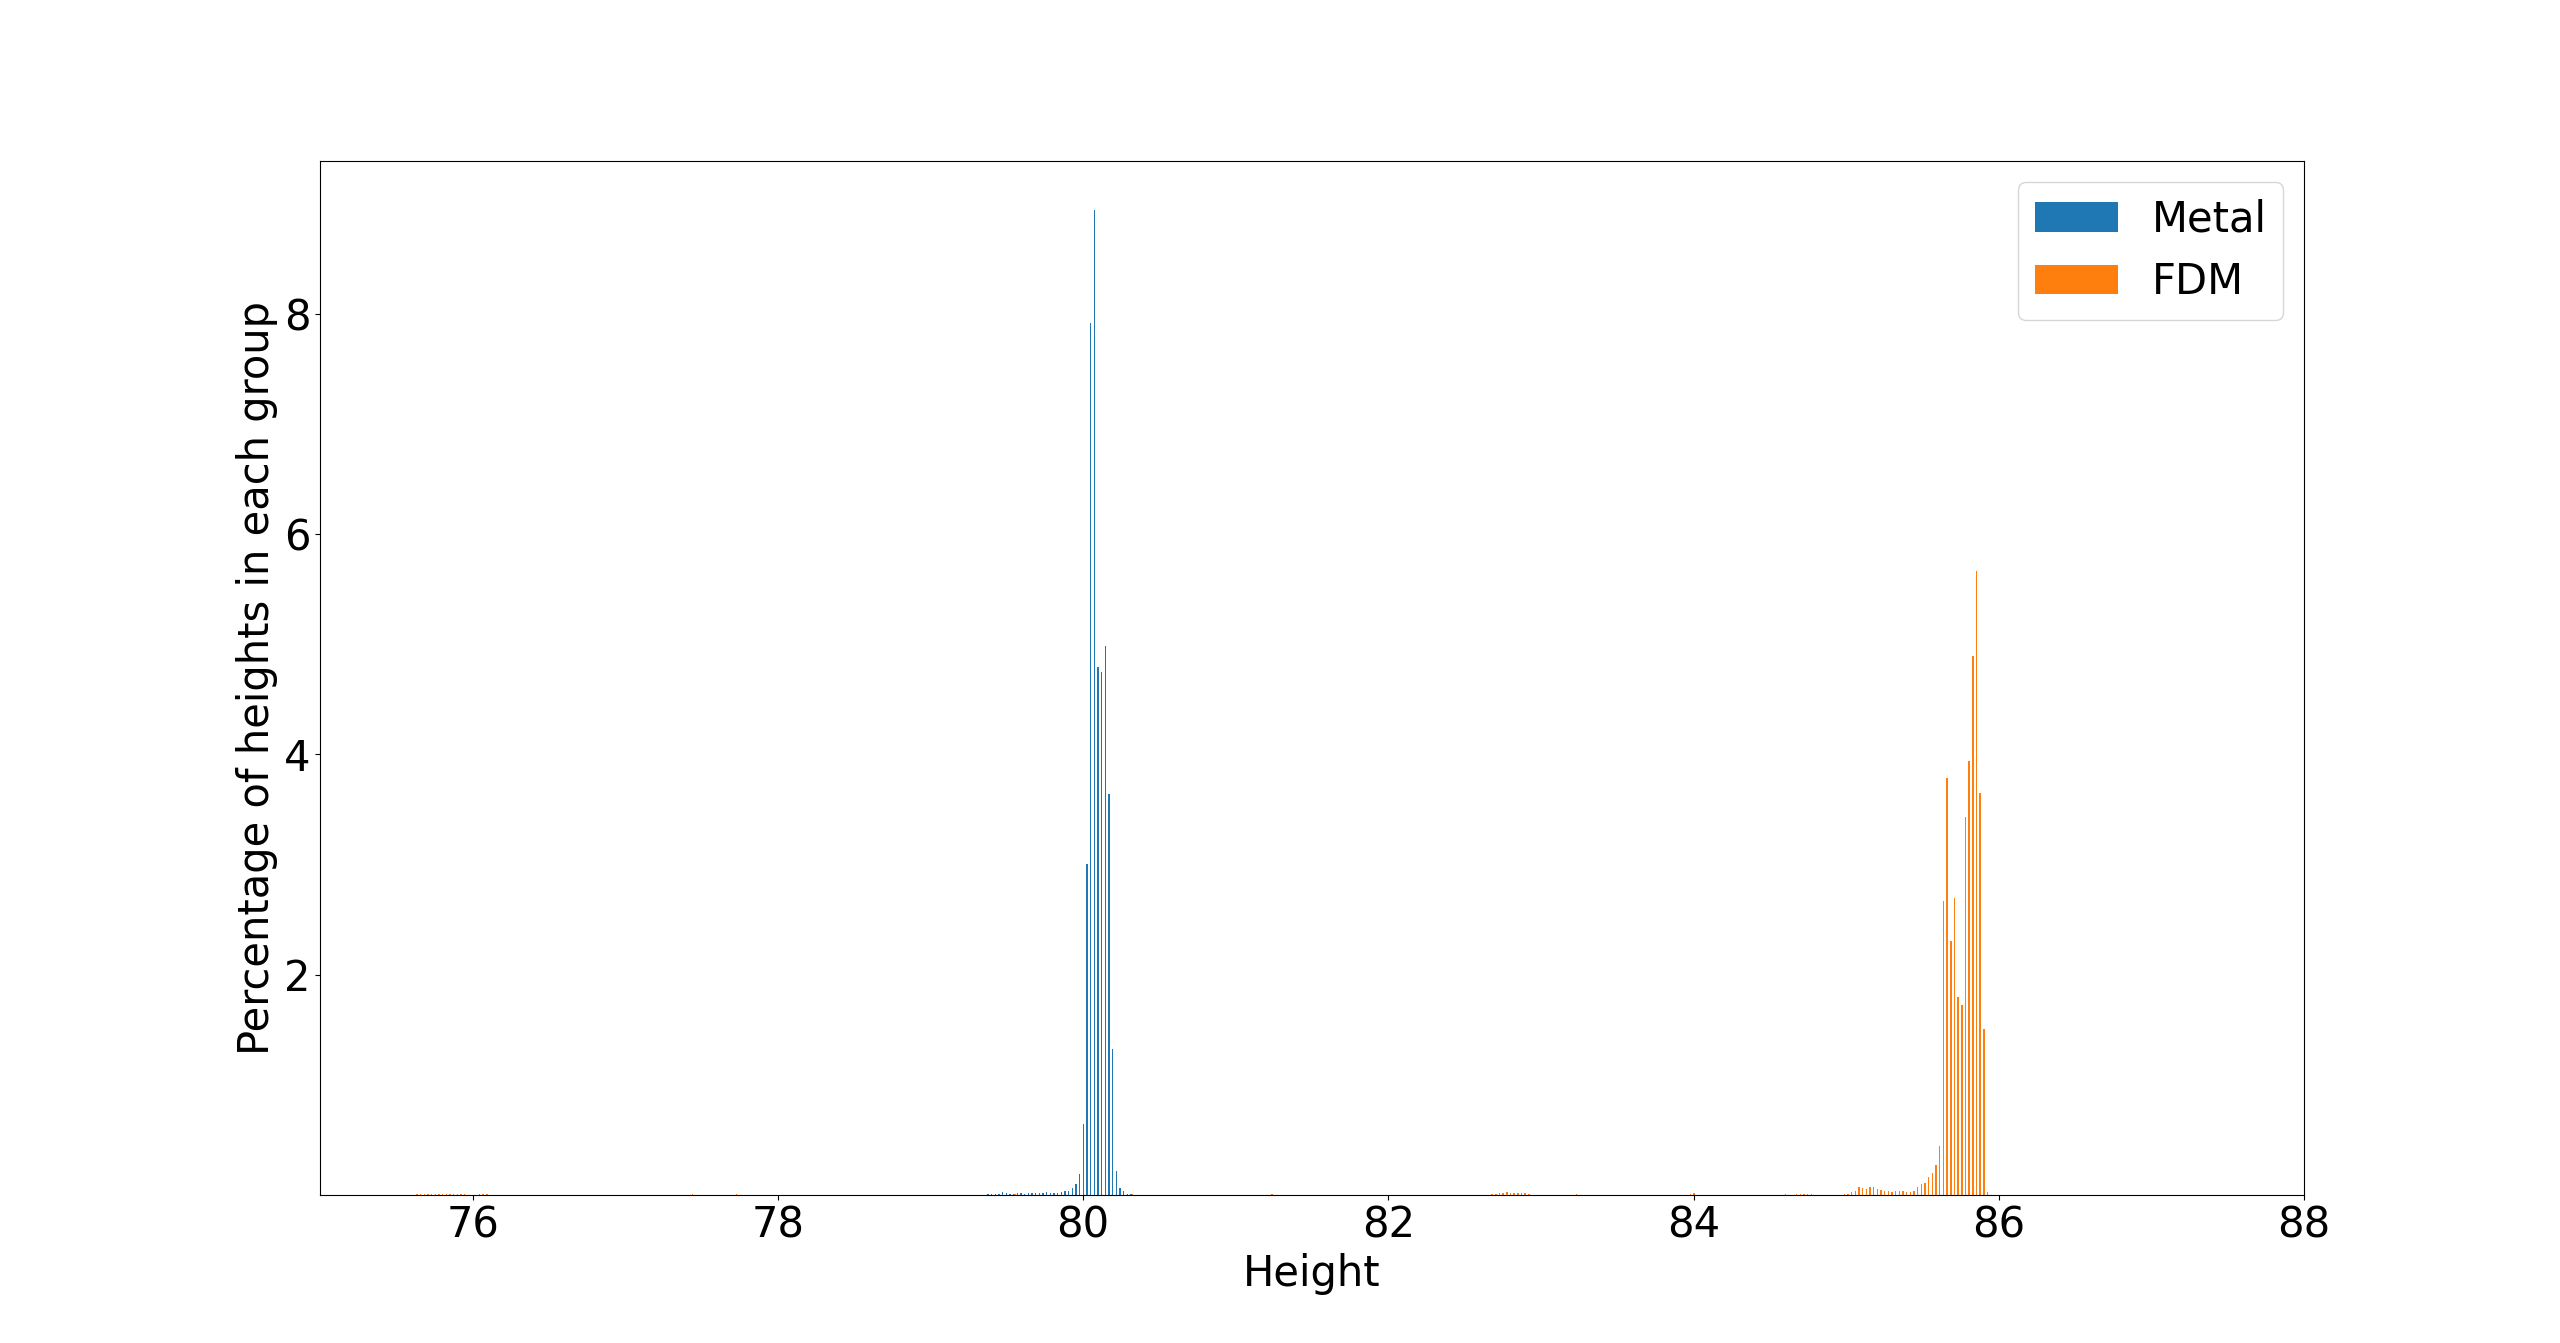
\includegraphics[width=0.5\textwidth]{images/height_occurange.png}
    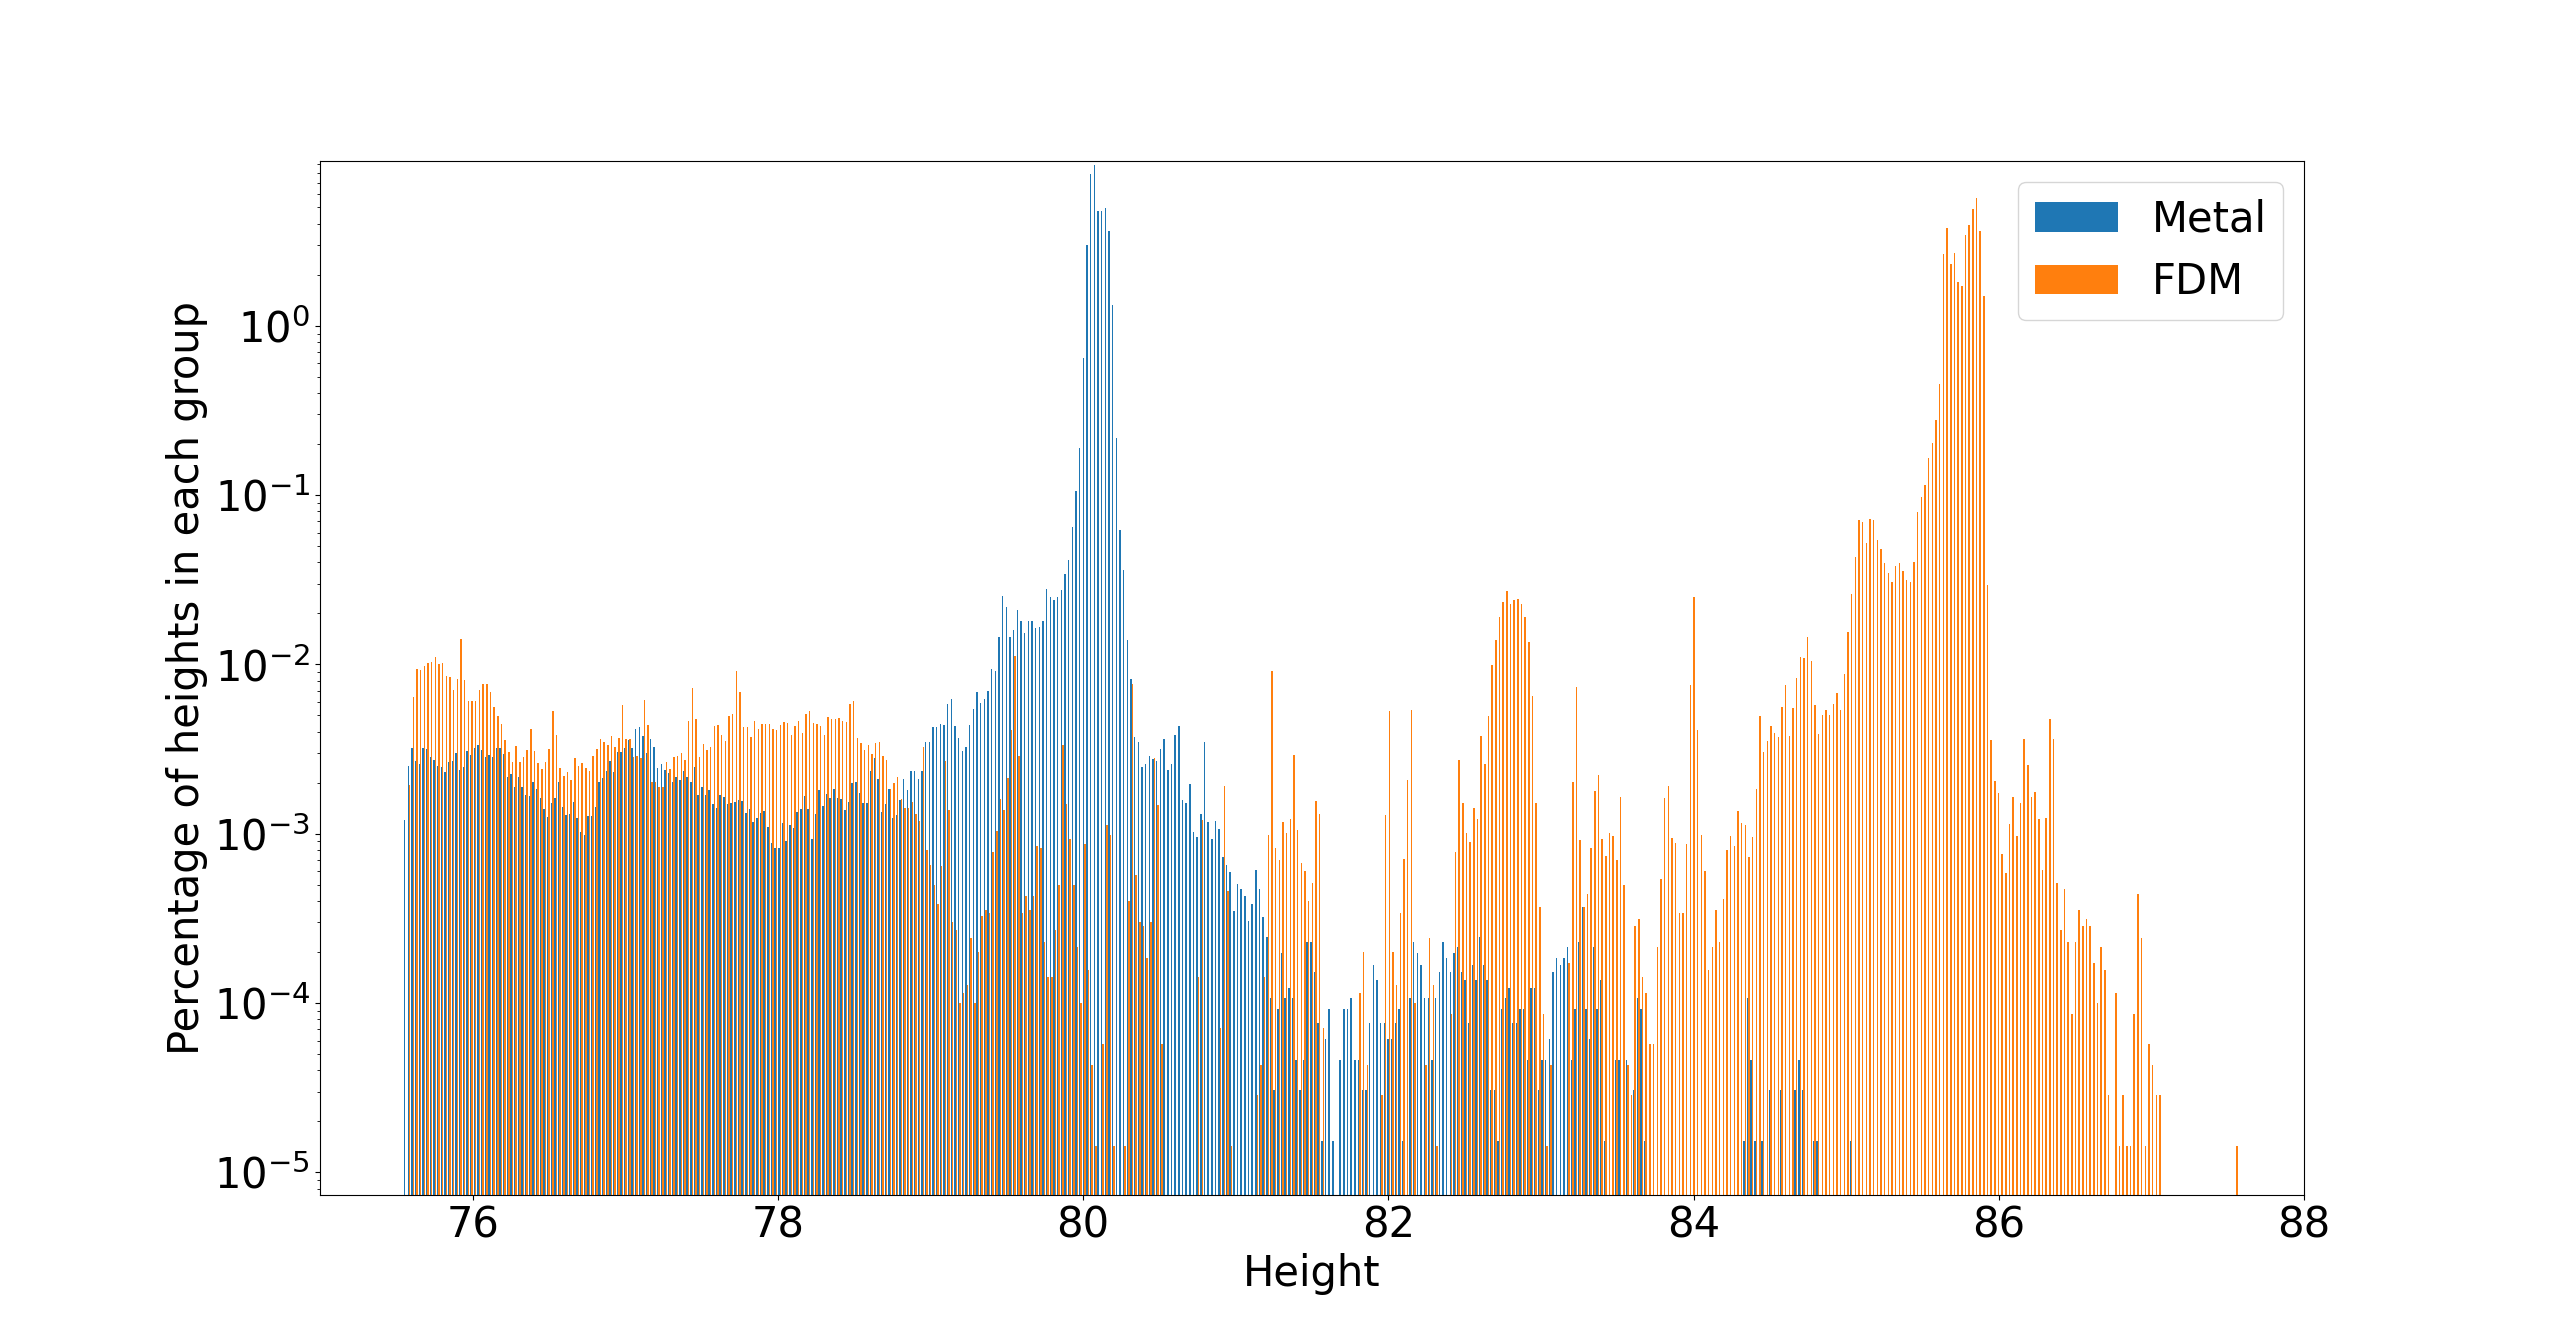
\includegraphics[width=0.5\textwidth]{images/height_occurange_log.png}
    \caption{Auftreten Höhe}
    \label{fig:brightness}
\end{figure}

Wie man in Abbildung \ref{fig:brightness} sehen kann streuen nicht alle Pointclouds 
gleich, abhängig von dem Werkstoff des Bauteils werden die Laserstrahlen unterschiedlich
reflektiert und mehr oder weniger Ausreißer sind zu sehen. 
Man sieht das Metallteil deutlich mehr in beide Richtungen 
streut, während das FDM gedruckte Bauteil weniger nach oben, aber mehr nach unten 
streut. Es muss also eine Filtermethode gewählt werden die für alle Fertigungsverfahren
anwendbar ist und nicht bei einer Methode besser funktioniert wie bei einer 
anderen. Werden zum Beispiel die 10 Prozent häufigst aufkommenden Höhenwerte bei einem
Metallteil benutzt kommt folgendes Bild heraus.

\begin{figure}[h]
    \centering
    \includegraphics[width=0.4\textwidth]{images/am_sp0_top_10p.png}
    \caption{Metallteil gefiltert}\label{fig:metall_image}
\end{figure}

Man sieht vor allem auf der rechten Seite, dass Ränder nicht mehr klar erkennbar sind, 
da sie durch die Filterung Lücken aufweisen. Praxistest haben gezeigt das ein 
ausreichend gut funktionierender Filterwert 50 Prozent ist. Damit werden genug 
Messfehler aus dem Bild genommen aber trotzdem bleiben Oberflächenfeatures und Ränder
sichtbar genug um ein korrektes Zusammenfügen zu gewährleisten.
Dieses Filtern bezieht sich aber nur auf 2 dimensionale Bildinformationen.
Um bei dem Konvertieren noch weniger Punkte die nicht auf dem Bauteil liegen nicht in das Bild zu übernehmen, kann auch noch die Pointcloud gefiltert werden.
Hier kann ein einzelner Punkt relativ zu seinem Nachbarn im 3 dimensionalen Raum betrachtet werden, 
um so Ausreißer zu erkennen. Dafür sind in der Open-Source
Bibliothek 'Open3D' 2 Methoden vorhanden: Radius basiert oder auf Basis von 
statistischen Werten, erste Methode eignet sich gut, wenn die Maße des Objekts bekannt
sind. Hier wird um jeden Punkt eine Kugel gebildet und die Punkte die weniger als 
einen konfigurierbare Menge an Punkte in ihrer Kugel haben werden entfernt. Da 
das hier zu entwickelnde Verfahren sich nicht auf eine Bauteilgeometrie beschränken
ist dieses Verfahren nicht geeignet. Stattdessen wird das andere benutzt. Hier werden
die Punkte entfernt die weiter von ihren benachbarten Punkten entfernt sind als der 
durchschnittliche Abstand der Punkte in der gesamten Pointcloud. Hier kann die Menge der 
benachbarten Punkte die betrachtet werden sollen und ein Limit für den Abstand von der 
Standardabweichung. Umso mehr benachbarte Punkte betrachtet werden, umso mehr Zeit 
braucht die Filterung, aber die Filterung wird auch akkurater. Im Praxistest haben sich
hier 50 Nachbarpunkte bewährt. Mit diesem Wert werden bei Pointclouds in unserem 
Datensatz jeweils ca. 2 Prozent der Punkte entfernt. So kann das resultierende
Bild gut genug umgewandelt werden, um eine erfolgreiche Zusammenführung 
von verschiedenen Bildern zu gewährleisten.
Ein Nachteil bei der Filterung in Abbildung \ref{fig:image_from_pc} links und rechts 
mittig zu sehen. Hier sind schwarze Punkte sichtbar. Diese treten auf, weil der Scanner
hier über dem Bauteil Punkte erkannt hat. Durch das Filtern wurden diese Punkte entfernt
beziehungsweise bei der Konvertierung nicht berücksichtigt. Da diese Punkte dann fehlen
bleiben sie im resultierenden Bild schwarz. Das ist zwar etwas unschön anzuschauen, 
beeinträchtigt das zusammenfügen aber nicht weiter. 

\subsection{Pointcloud in Bild konvertieren}

Um Rechenzeit zu sparen und auf viele Funktionen von schon bestehenden 
Bilderkennungs-Bibliotheken zurückgreifen zu können habe ich die Pointclouds in ein
Bild konvertiert. Hierfür wird zuerst in leeres Bild mit den gleichen Maßen einer 
Pointcloud erstellt. Dann wird über alle Punkte der Pointcloud iteriert und jeweils
der Pixel an der X und Y Koordinate des Punktes auf einen Helligkeitswert gesetzt.
Um Rechenzeit und Speicherkapazitäten zu schonen, und weil es für die Berechnung 
ausreichend ist, habe ich mich für 8 Bit Single-Channel Bilder die nur Helligkeitswerte 
abbilden entschieden. Hier kann also jede Pixel einen Wert zwischen 0 und 255 annehmen.
Der entsprechende Wert kann wie folgt berechnet werden:

\begin{equation*}
    value_p = \frac{Z - min_z}{max_z - min_z} \cdot (max_{brightness} - min_{brightness}) + min_{brightness}
\end{equation*}

Der resultierende Wert ist die Helligkeit, die dem Pixel zugewiesen wird.
$Z$ ist die Z-Koordinate des Punktes in der Pointcloud. $min_y$ und $max_y$ sind 
die Grenzen der Z-Koordinate, diese werden gebraucht um die Helligkeit relativ 
zu der Höhe zu berechnen. $min_b$ und $max_b$ sind die gewünschten Grenzen der 
Helligkeit. In unserem Fall sind $min_b = 0$ und $max_b = 255$ da ein 8 Bit Bild
verwendet wird.

\begin{figure}[h]
    \centering
    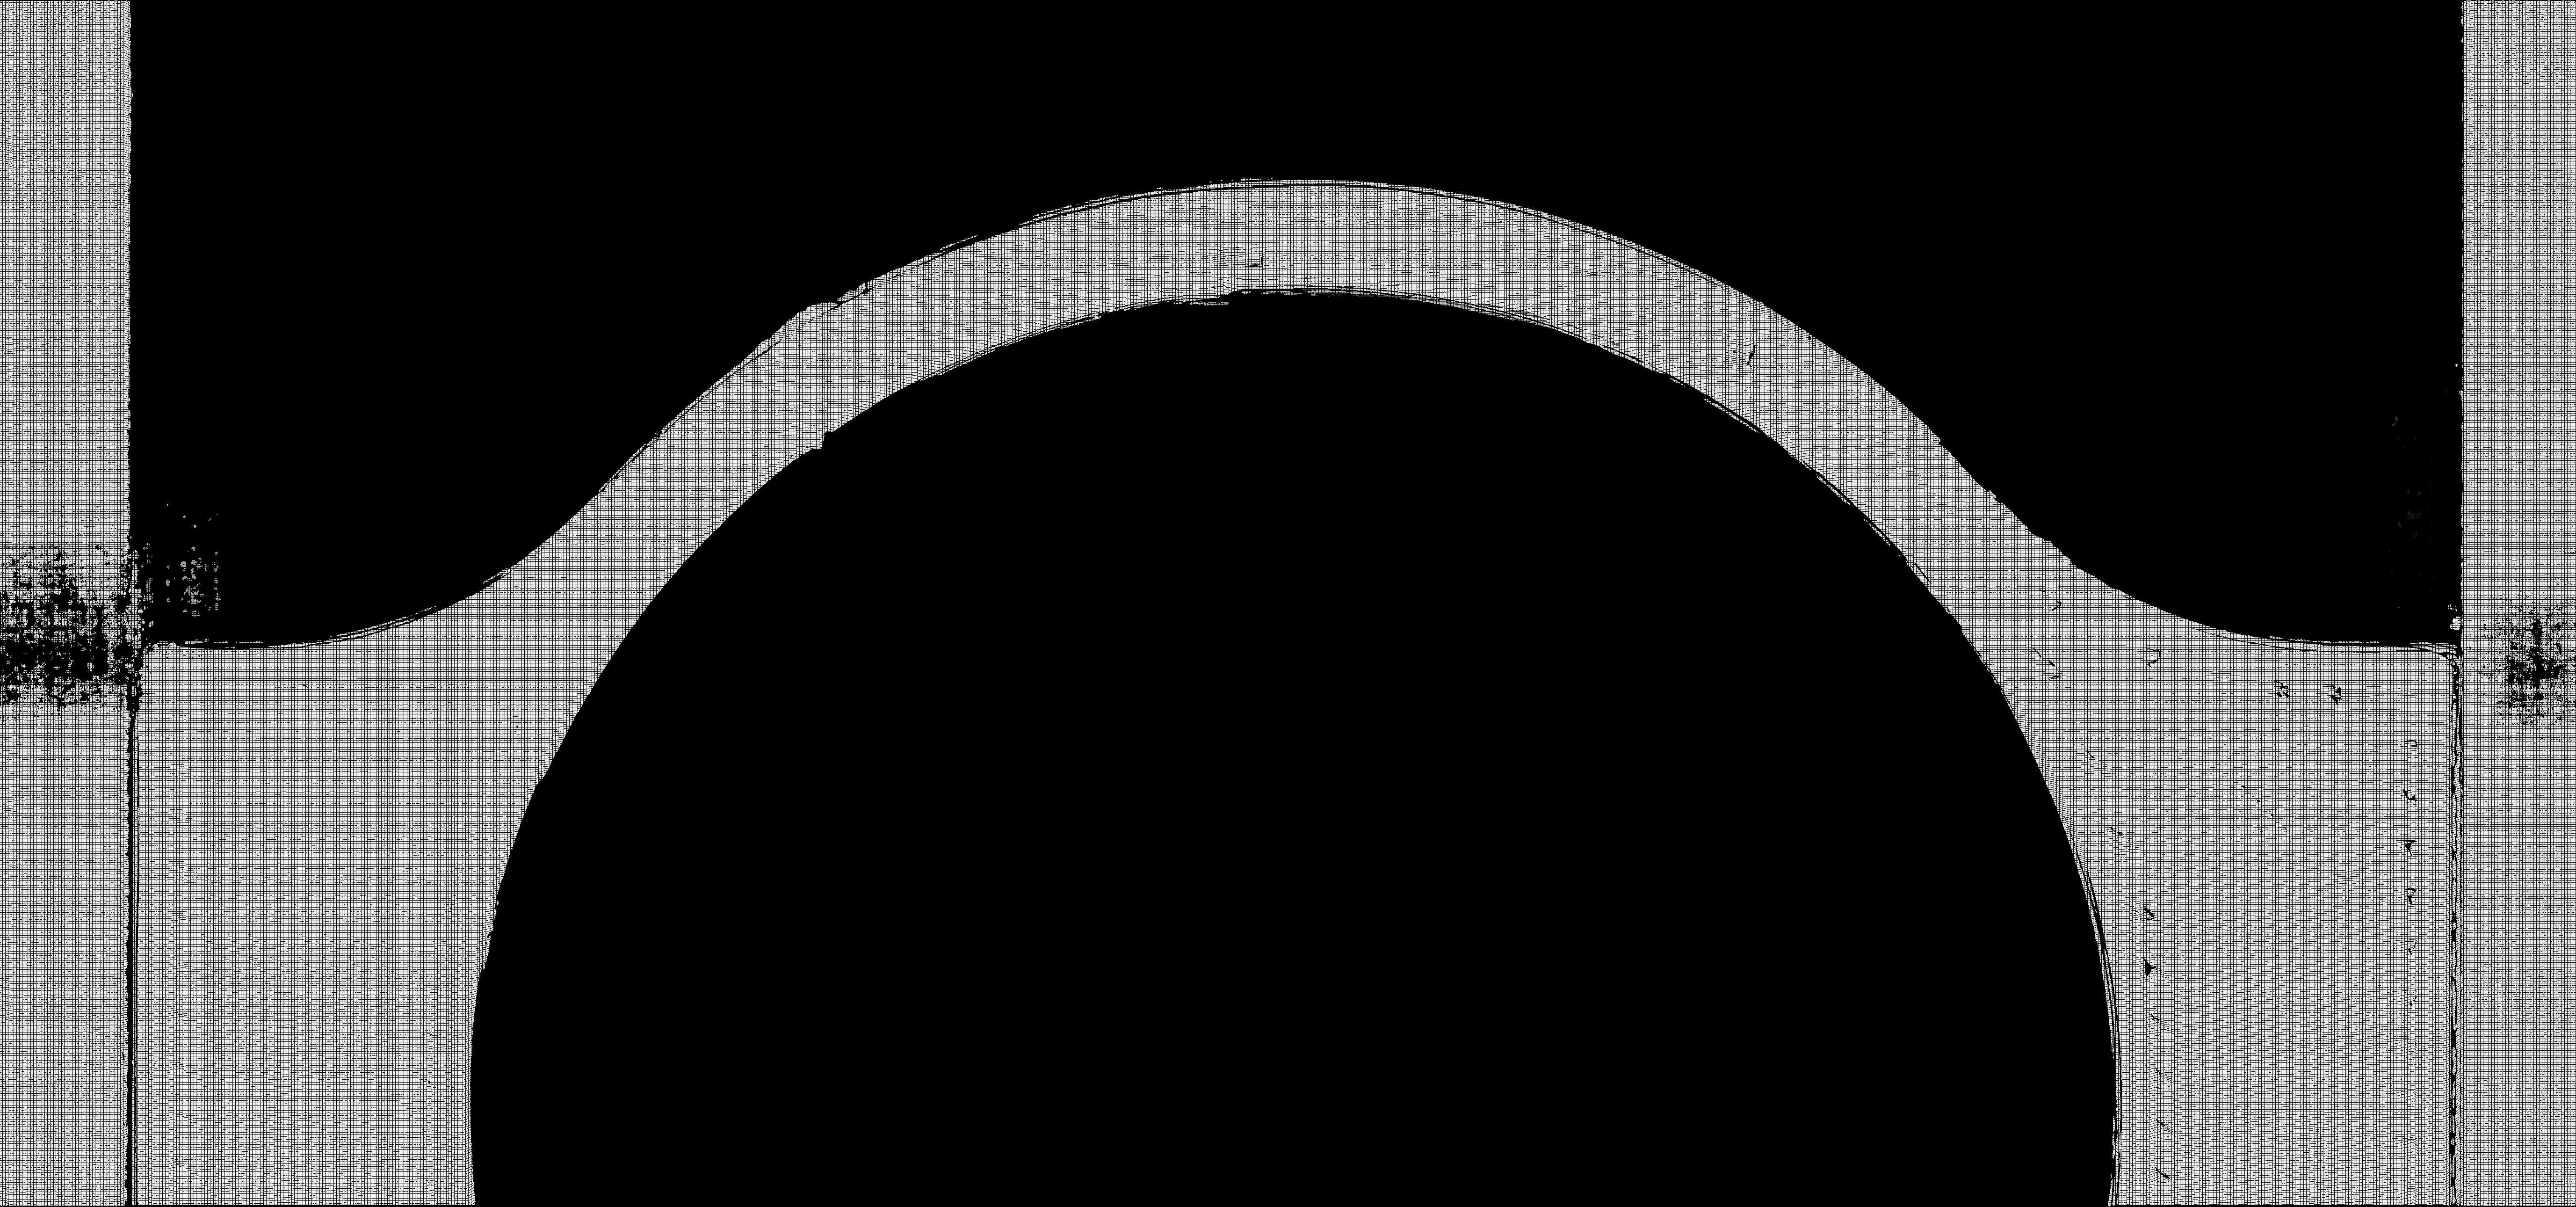
\includegraphics[width=0.5\textwidth]{images/fdm_top_100p.png}
    \includegraphics[width=0.5\textwidth]{images/fdm_top_10p.png}
    \caption{Konvertierung Pointcloud zu Bild}
    \label{fig:image_from_pc}
\end{figure}

Wie man in Abbildung \ref{fig:image_from_pc} sehen kann, sind kaum Helligkeitsveränderungen
im Bild sichtbar. Das liegt an derselben Problematik, an der der ICP-Algorithmus häufig
scheitert. Reale Datensets wie wir es vorliegen haben sind nicht perfekt, sondern
beinhalten Messfehler und Streuungen. 

Abbildung \ref*{fig:brightness} zeigt die Häufigkeit der gleichen Höhenwerte einer
Pointcloud von dem Demonstratorbauteil. In Blau ist die Verteilung der Punkte auf 
einem Demonstratorbauteil zu sehen das aus Metall gedruckt wurde, Orange zeigt die 
Verteilung der Punkte auf einem Kunststoffteil.
In dem oberen Histogramm 
sind die Häufigkeiten der Höhenwerte zu sehen. Der Datensatz wurde in 500 gleich große
Teile gruppiert, jeder Balken repräsentiert eine Gruppe.
Unterhalb ist das Histogramm mit dem gleichen Datensatz, aber mit der y-Achse 
logarithmisch skaliert um kleine Prozente deutlich zu machen die im
oberen Diagramm nur schwer oder gar nicht sichtbar sind. 
Die meisten Höhenwerte treten bei ca. 80 beziehungsweise 85 auf, 
sie gehören zu den Punkten, die auf dem Demonstratorbauteil liegen, 
es treten allerdings auch Werte darunter und darüber auf. 
Die in Abbildung \ref*{calc:brightness} vorgestellte Formel benutzt allerdings 
die absoluten Minimum und Maximum Werte.
Alle Punkte die tatsächlich auf dem Bauteil werden also entsprechend wenig
berücksichtigt. Dem kann Abhilfe geschaffen werden, indem Werte, die weniger häufig 
auftreten entfernt werden. Sortiert man alle Höhenwerte nach der Häufigkeit ihres 
auftreten in der Pointcloud und entfernt den n-ten Prozentsatz können Ausreißer 
entfernt werden. Wenn nur die häufigsten 10 Prozent übernommen werden erhält man 
das untere Bild in Abbildung \ref{fig:image_from_pc}

Features auf dem Bauteil können jetzt deutlich besser erkannt werden. Auch zu sehen
sind jetzt die Markierungen auf der linken und Rechten Seite die bei der Registrierung
helfen sollen. Auch schön zu sehen sind die Spuren und Lücken die durch den FDM 
Herstellungsprozess entstehen.

Durch das Filtern der Höheninformationen sind Oberflächenstrukturen nicht nur besser
erkennbar, auch die Ränder treten genauer hervor. 
Dadurch können mehrere Bilder korrekt zusammengefügt werden.

\end{document}

\newpage

\documentclass[../main.tex]{subfiles}
\begin{document}

\section{Stitching}


\end{document}

\newpage

\documentclass[../main.tex]{subfiles}
\begin{document}

\section{Analyse der spannkraftinduzierten Deformation}



\end{document}

\newpage


\chapter{Anwendung und Algorithmus}

Ziel dieser Arbeit ist es nicht nur eine Methodik zur optische 
Deformationserkennung zu entwickeln, sondern diese Methodik auch in einer 
Anwendung einfach nutzbar zu machen. 

Diese Kapitel dokumentiert diese Anwendung und geht auf Herausforderungen 
in der Entwicklung ein.

\section{Anwendung}

Die Anwendung beeinhaltet verschiedene Funktionen, alle Funktionen 
können separat benutzt werden. Dadurch müssen zeitintensive Vorgänge nicht 
wiederholt werden, sondern Zwischenergebnisse können abgespeichert und 
neu geladen werden.
Die Anwendung bietet Funktionen um Resultate in dem entsprechenden Dateiformat zu 
speichern. Soweit möglich werden Dateinamen Empfehlungen automatisch ermittelt, 
daher ist es zu empfehlen von Anfang an mit einem einheitlichen Namensschema bei
den 3D-Scannerdaten zu arbeiten. 
Das Schema \glqq Bauteilbeschreibung \textunderscore Spannungsstufe\grqq~~
\textunderscore Scannerdurchlauf.ply
wird empfohlen. Ein Beispiel für die zweite Pointcloud eines FDM-Bauteil bei der
vierten Spannungsstufen wäre also \glqq FDM0\textunderscore SP4\textunderscore 2.ply\grqq~.
In Abbildung \ref{fig:software_screenshot} ist die Oberfläche der Anwendung zu sehen.

\begin{figure}[H]
    \centering
    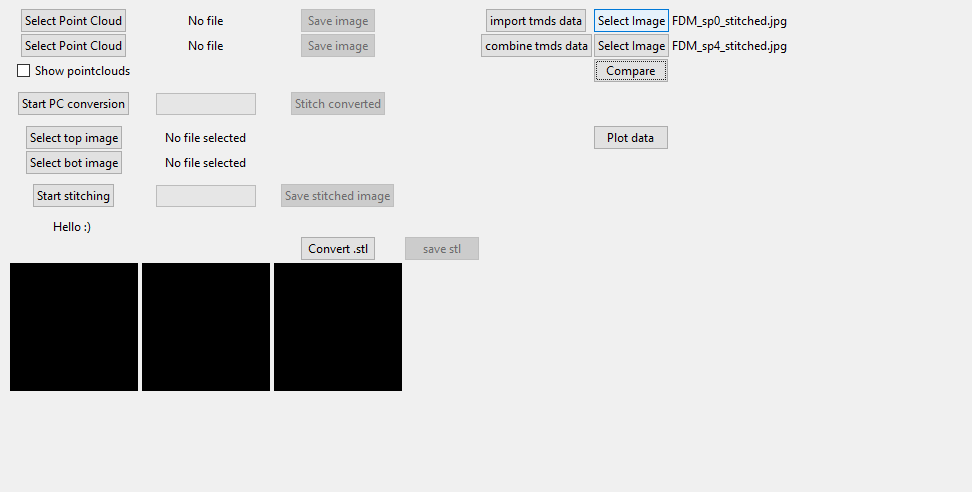
\includegraphics[width=0.9\textwidth]{images/software_screenshot.png}
    \caption{Anwendungsoberfläche}
    \label{fig:software_screenshot}
\end{figure}

Über die Buttons \glqq Select Pointcloud\grqq~ können Pointclouds zum Konvertieren in Bilder
ausgewählt werden. Der Text neben dem Bild zeigt den Dateinamen der ausgewählten 
Datei an. Die obere Pointcloud sollte hier als erstes ausgewählt werden.
Der Button \glqq Start PC conversion\grqq~~startet die Konvertierung. Der Balken 
daneben zeigt den Prozessfortschritt. 
Wenn \glqq Show Pointclouds\grqq~ gesetzt ist, werden die Pointclouds vor dem 
Konvertieren in einem separaten Fenster angezeigt. So kann überprüft werden, ob die 
korrekte Pointcloud ausgewählt wurde.
Wenn der Prozess abgeschlossen ist, werden die resultieren Bilder als Vorschau in der 
Anwendung angezeigt und die Option zum Speichern der Bilder ist nicht mehr ausgegraut.
Zusätzlich wird nach dem Konvertierungsprozess die Schaltfläche 
\glqq Stitch converted\grqq~ freigeschaltet. Durch diese Option können die 
Bilder direkt zusammengefügt werden, ohne das die Bilder extra gespeichert und 
eingeladen werden müssen. Wenn schon existierende Bilder zusammengefügt werden sollen, 
können die Schaltflächen \glqq Select top image\grqq und \glqq Select bot image\grqq
ausgewählt werden um das obere und untere Bild auszuwählen. Auch hier wird die 
ausgewählte Datei als Text angezeigt. Die Dateiauswahl erfolgt über das 
Windows-Kontextmenü, der zuletzt verwendete Ordner wird hierbei erhalten, sodass das 
zweite Bild schneller ausgewählt werden kann. 
Über den Button \glqq Start stitching\grqq wird der stitching Prozess gestartet. 
Auch hier wird der Fortschritt und das Endresultat, sobald es vorliegt, angezeigt.

Damit auch die CAD-Datei des additiv gefertigten Bauteils verglichen werden kann, 
existiert der \glqq Convert stl\grqq~ Button. Hier wird eine .stl Datei zu einem Bild 
konvertiert und kann über \glqq save stl\grqq~ gespeichert werden.

Mithilfe der rechts zu sehenden Schaltflächen können Bilder auf ihre Deformation hin 
verglichen werden. Die resultieren Deformationsdaten werden automatisch als Textdatei
in dem Ordner \glqq deformation\underline data\grqq~ gespeichert. Dieser Ordner wird automatisch 
in dem Verzeichnis erzeugt, in dem die Anwendung ausgeführt wird. 
Die erstellten Textdateien können mithilfe des Buttons \glqq Plot data\grqq~ ausgewählt 
werden, und werden automatisch als Graph angezeigt. 

Beim konvertieren und stitchen werden alle Prozesse, die nicht voneinander abhängig sind,  
nebenläufig ausgeführt. Das reduziert die Laufzeit der Prozesse.

Die Anwendung ist in Python geschrieben, rechenintensive Prozesse wurden aber mithilfe 
der Bibliothek \glqq Numba\grqq~in optimierten Maschinencode compiliert~\cite{numba}.
Dadurch ist der Konvertierungs- und Stitching-Prozess deutlich schneller geworden. 
Abbildung \ref{label} zeigt die Laufzeiten der Anwendung mit und ohne Übersetzung in 
Maschinencode.

[TODO: Bild laufzeiten einfügen]





\newpage

\documentclass[../main.tex]{subfiles}
\begin{document}

\section{Zusammenfassung und Ausblick}


\end{document}

\newpage


\chapter{Validierung}

Im folgenden Kapitel wird die Deformationerkennung analysiert und überprüft.
Zur Überprüfung werden Materialeigenschaften und aufgenommene Messwerte 
mit der erkannten Deformation verglichen.

\section{Messergebnisse}

Es wurden fünf Bauteile mit verschiedenen Spannungsstufen gemessen. Für jede 
Spannungsstufe wurde die Kraft, die auf das Bauteil wirkte sowie die Verschiebung 
des Schraubstocks gemessen.
Jede Spannungsstufe wurde durch Stufenweises anziehen des Schraubstocks erreicht.
Die Spannkraftkurve eines einzelnen Einspannvorgangs ist in 
Abbildung \ref{fig:single} zu sehen. 
In der Spannungskurve ist ein elastischer Bereich für das 
Bauteil zu sehen, in dem sich die Spannkraft zurückbewegt, nachdem kein 
Anzugdrehmoment mehr anliegt. Aus diesem Grund kann nicht der maximale Wert der Spannkraft angenommen werden, 
sondern es muss ein Wert gewählt werden der nach dem maximalen Ausschlag liegt.
Dieser wurde über die erste Ableitung der Spannkraftkurve gefunden. Sobald der 
Absolutwert der Steigung unter 0.0009 N fällt, wir die Spannkraft und Auslenkung an 
diesem Punkt gewählt. 0.0009 N wurde empirisch ermittelt, um bei allen Bauteilen einen 
angemessenen Wert zu liefern.
Die Spannkraft wurde an zwei Achsen aufgenommen und zu der Gesamtkraft aufsummiert.

\begin{figure}[H]
    \centering
    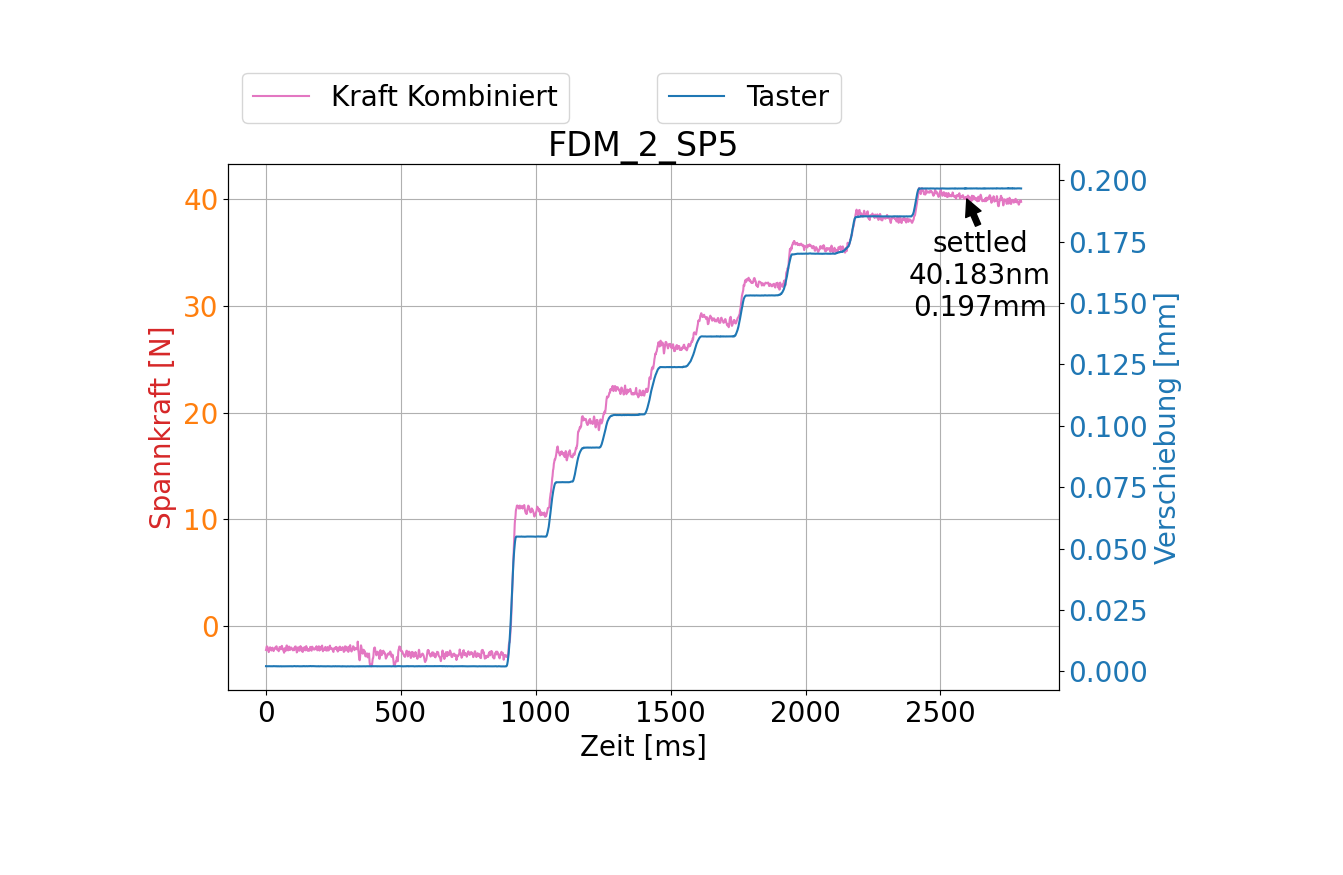
\includegraphics[width=0.99\textwidth]{images/spannkraftstufen_single.png}
    \caption{Kraft- und Verschiebung der Spannungsstufe fünf bei einem FDM Bauteil}
    \label{fig:single}
\end{figure}

Diese maximalen Werte für die Spannkraft und Auslenkung wurden für jedes Bauteil 
akkumuliert und sind in Abbildung \ref{fig:akkumulated} dargestellt. 
Die mit dem FDM-Prozess hergestellten Bauteile wurden jeweils in sechs Spannungsstufen
gemessen. Zwischen den Stufen wurde versucht, eine konstante Kraft auf das Bauteil 
auszuüben. Durch den manuellen Prozess des Anziehens des Schraubstocks war dies 
jedoch nicht immer möglich.
Die Metallbauteile unterscheiden sich durch ihren Aufbau. 
Alle basieren auf dem gleichen 3D-Modell, besitzen jedoch unterschiedliche 
Stützstrukturen. Im Bauteil AM0 ist die vollständige Stützstruktur vorhanden,
während in den Bauteilen AM1 und AM2 die Stützstruktur in unterschiedlicher 
Tiefe ausgebohrt wurde. Die Bauteile sind in Abbildung \ref{fig:am_parts} dargestellt.

Das Bauteil AM0 wurde nur mit zwei Spannungsstufen gemessen, 
da bereits bei der zweiten Stufe über 2500 N Kraft erforderlich war, 
um das Bauteil nur minimal in x-Richtung zu deformieren. Dies zeigt, 
dass die Stützstruktur einen erheblichen Einfluss auf die Verformbarkeit 
eines Bauteils hat. Beim Bauteil AM1 wurden 2500 N erst nach vier Spannungsstufen 
erreicht. Vergleicht man die Verformung in x-Richtung mit der Verformung von AM2,
 zeigt sich, dass das Bauteil ohne Stützstruktur bei ähnlicher Krafteinwirkung 
 etwa doppelt so weit in x-Richtung deformiert wurde.

 Die FDM-Bauteile wurden mit deutlich weniger Kraft eingespannt. 
 Hier wurde bei etwa 250 N gestoppt, dennoch ist die Verschiebung der 
 Teile deutlich größer als bei den AM-Bauteilen. Diese Werte wurden aufgenommen, 
 um die visuelle Deformationserkennung zu validieren.

\begin{figure}[H]
    \centering
    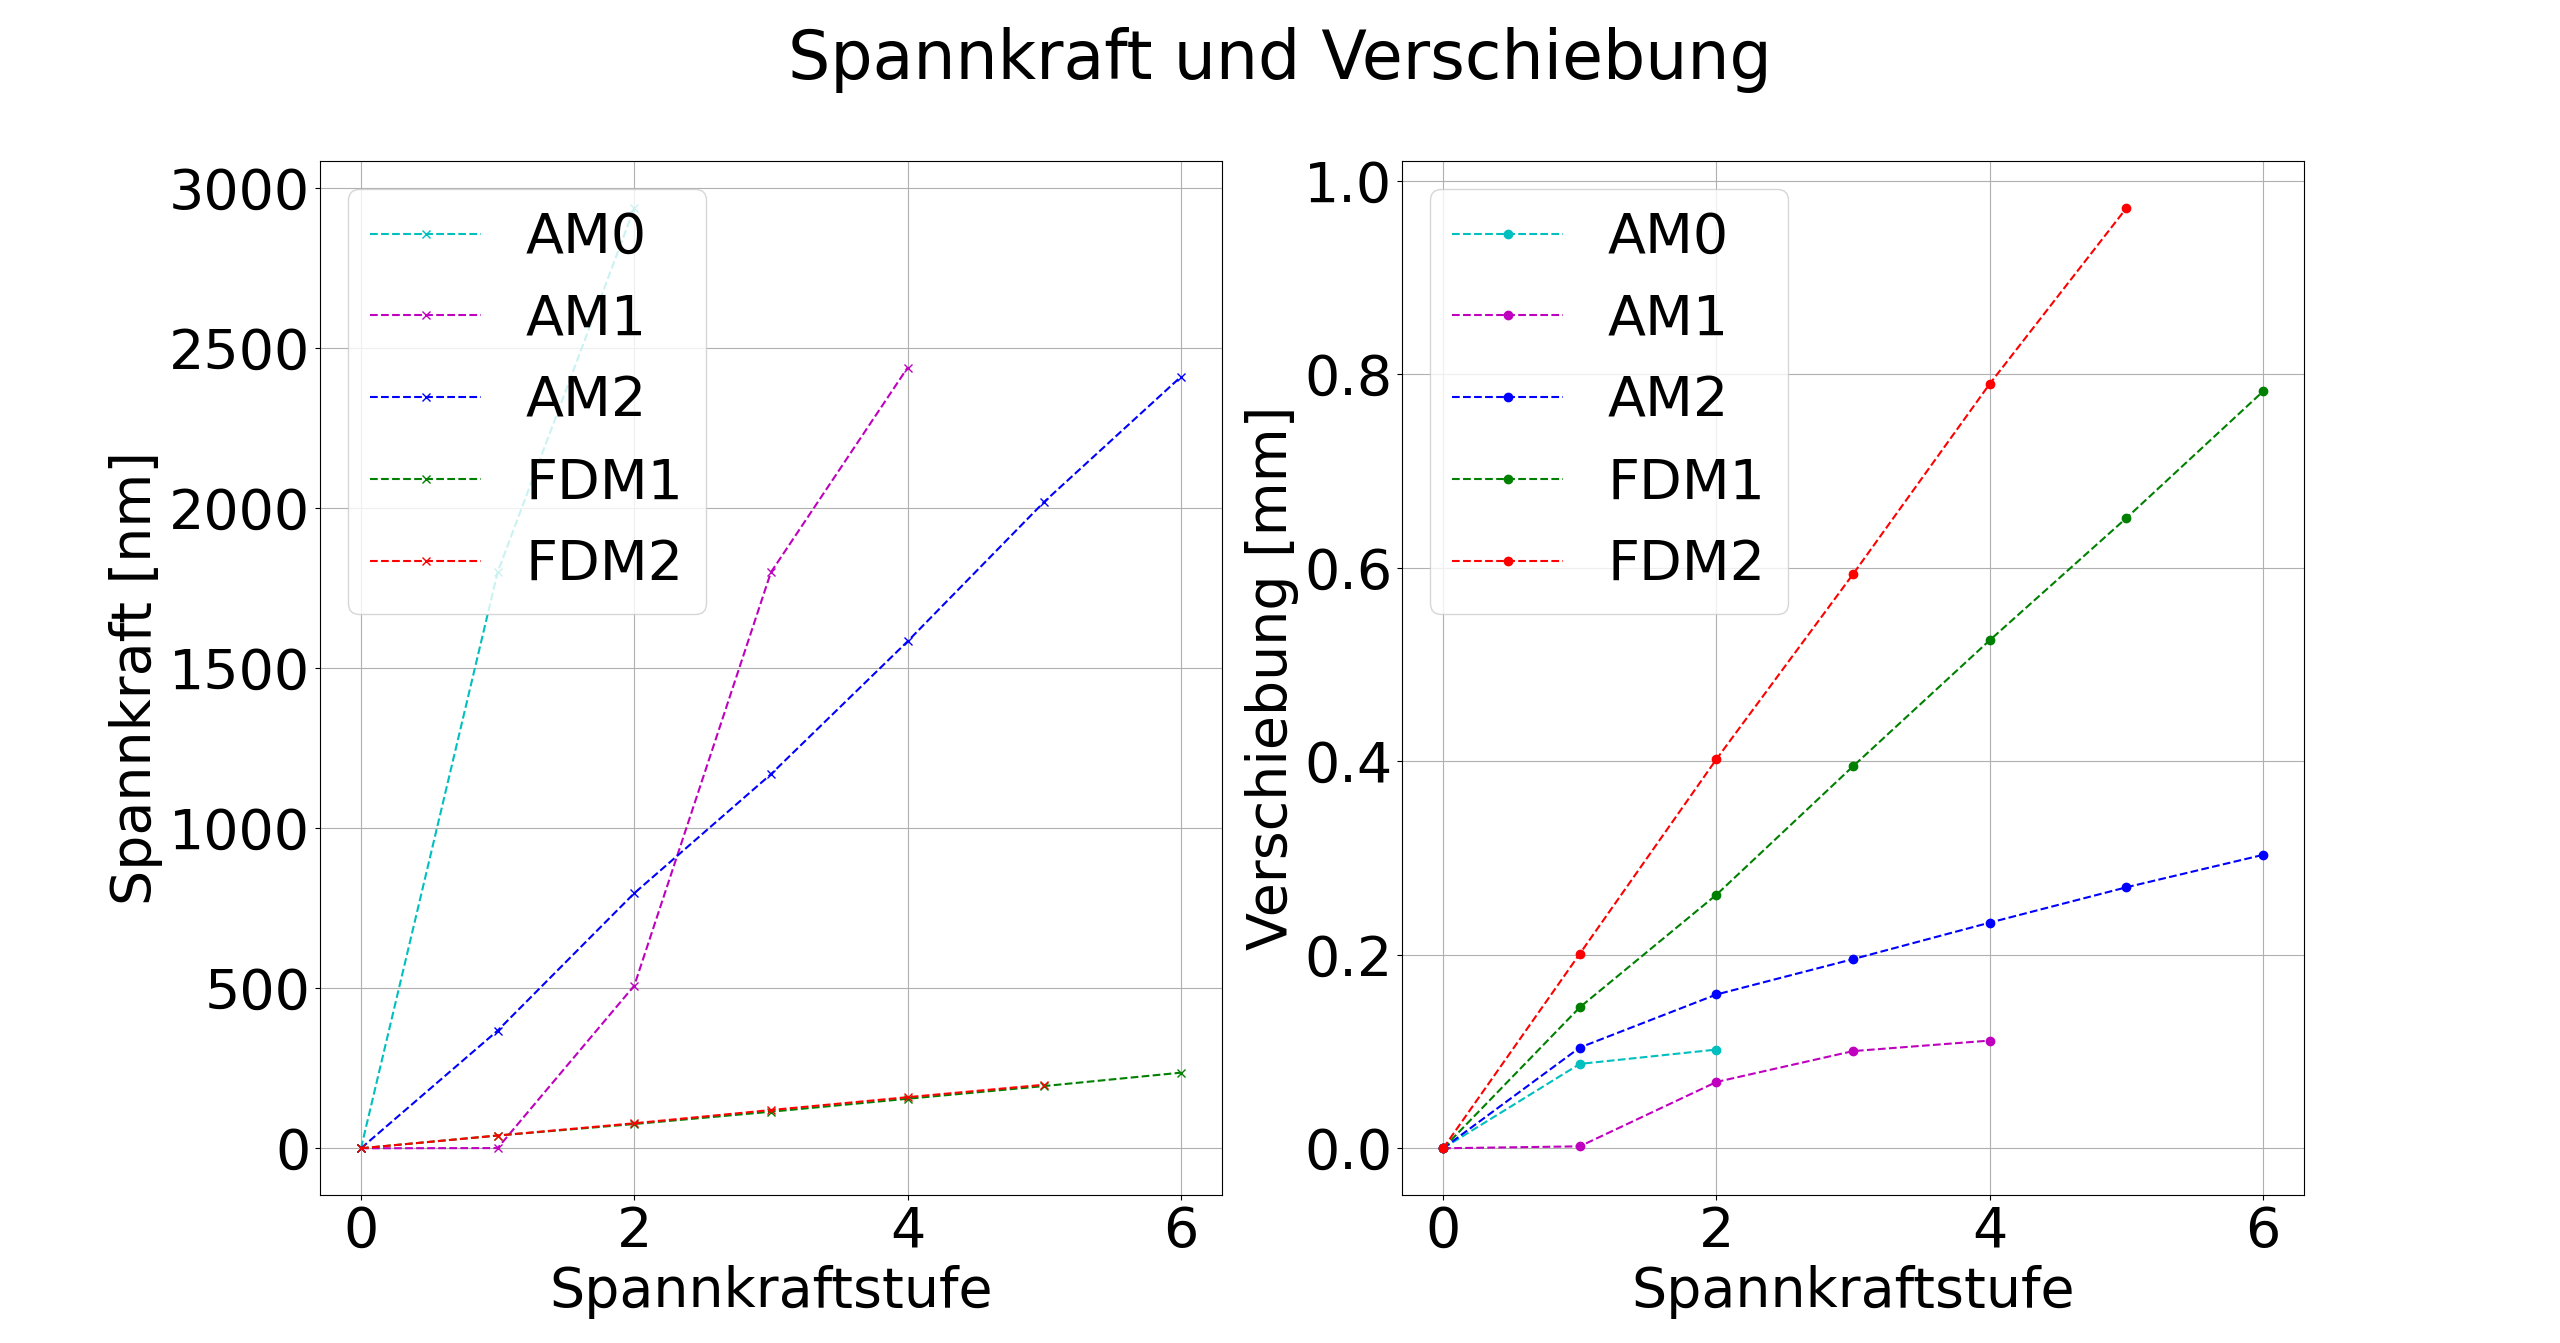
\includegraphics[width=0.99\textwidth]{images/spannkraftstufen_akkumuliert.png}
    \caption{Akkumulierte Kraft und Verschiebung, mit der jedes Bauteil deformiert wurde.}
    \label{fig:akkumulated}
\end{figure}

\begin{figure}[H]
    \centering
    \begin{minipage}{.33\textwidth}
      \centering
      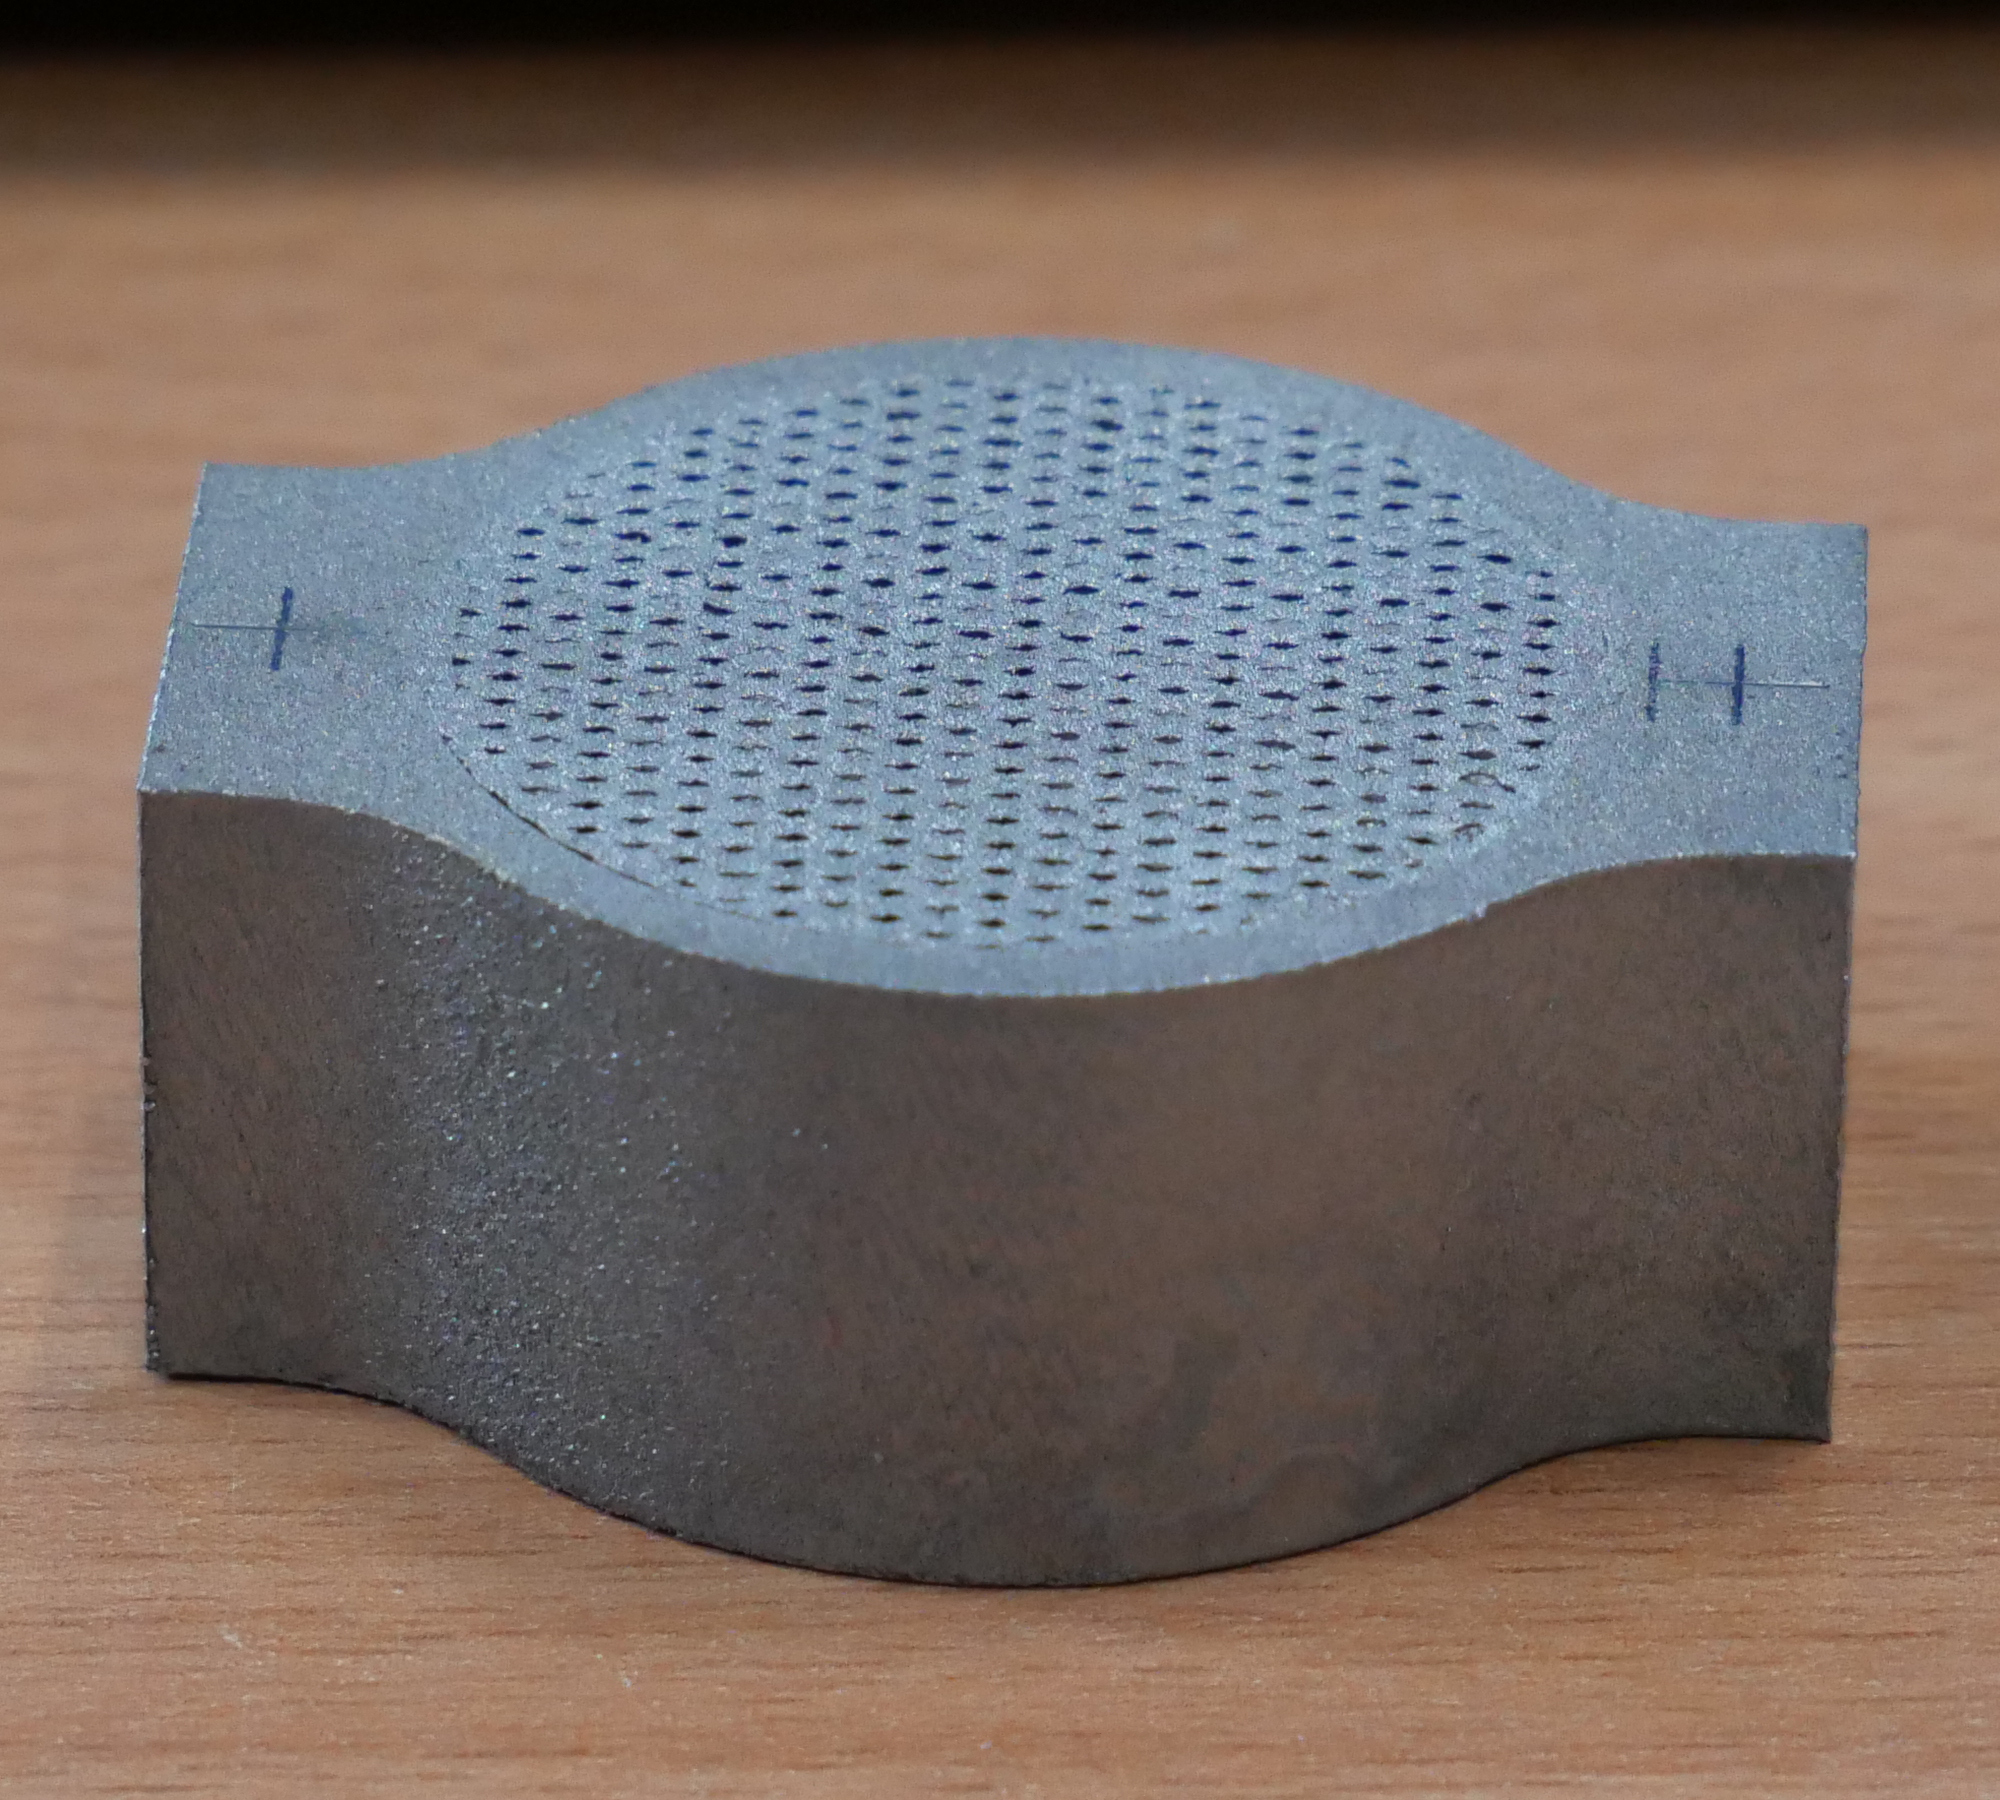
\includegraphics[width=0.9\linewidth]{images/AM0_crop.JPG}
      \caption*{(a)}
    \end{minipage}%
    \begin{minipage}{.33\textwidth}
      \centering
      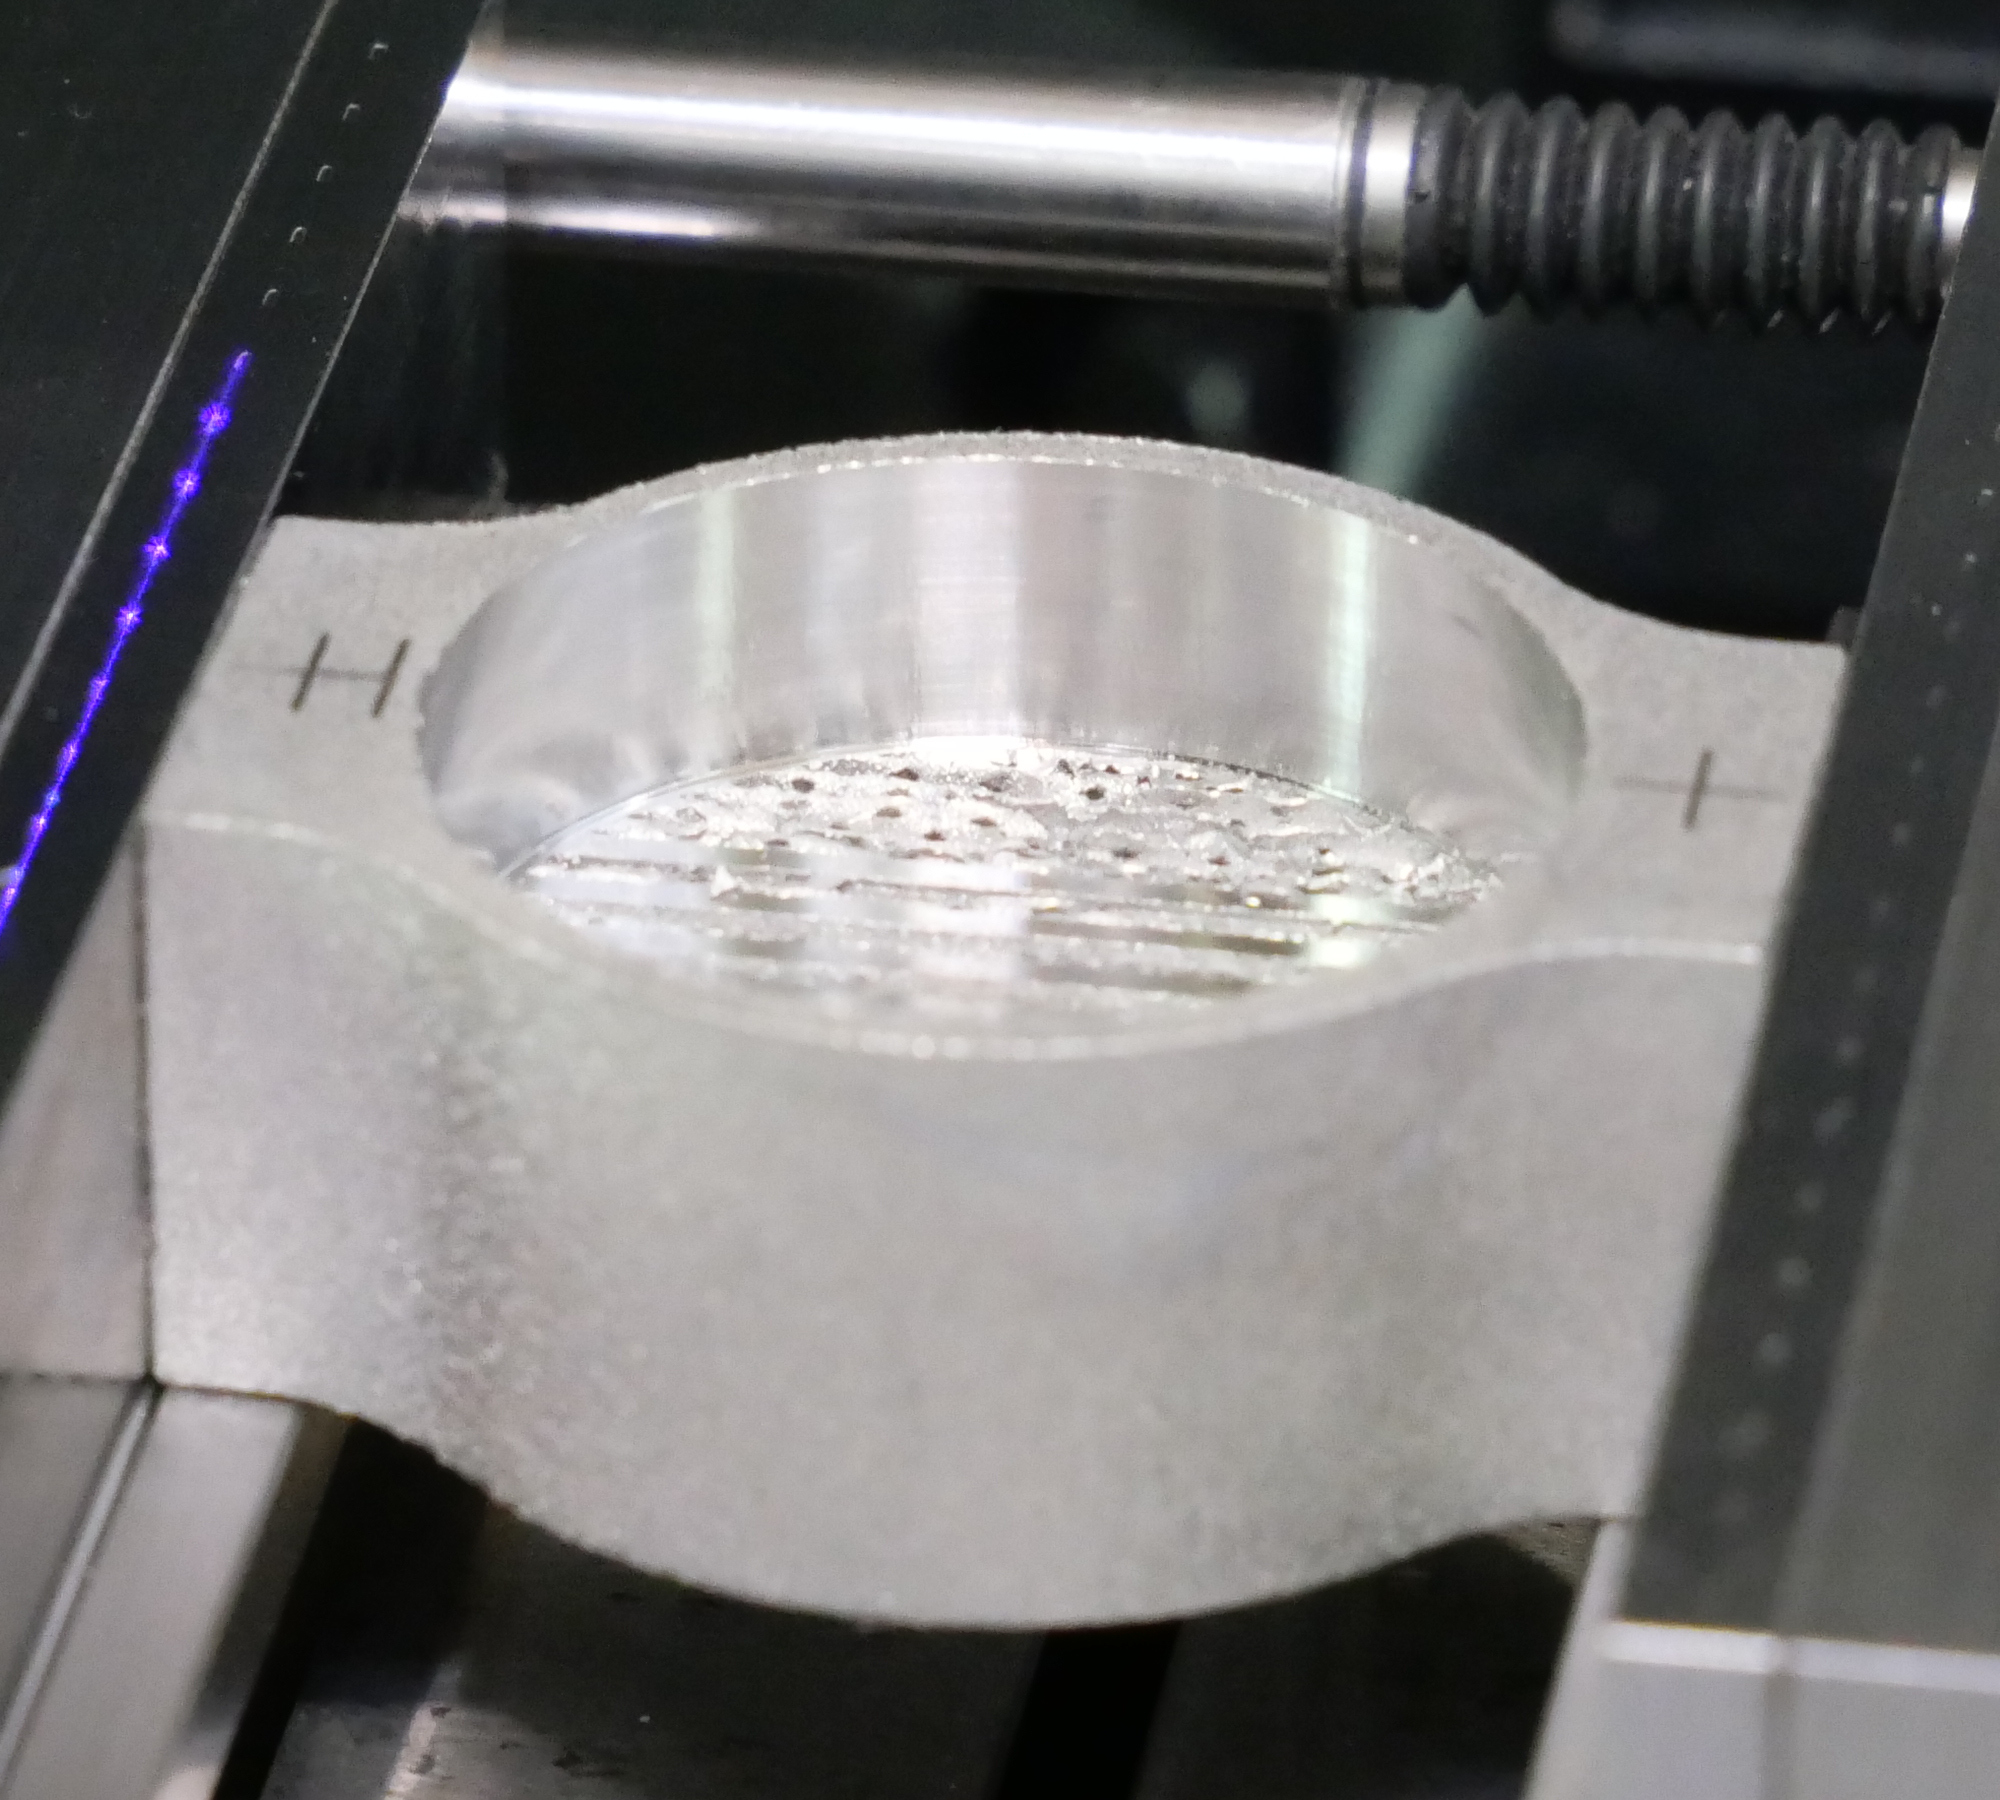
\includegraphics[width=0.9\linewidth]{images/AM1_crop.JPG}
      \caption*{(b)}
    \end{minipage}
    \begin{minipage}{.33\textwidth}
        \centering
        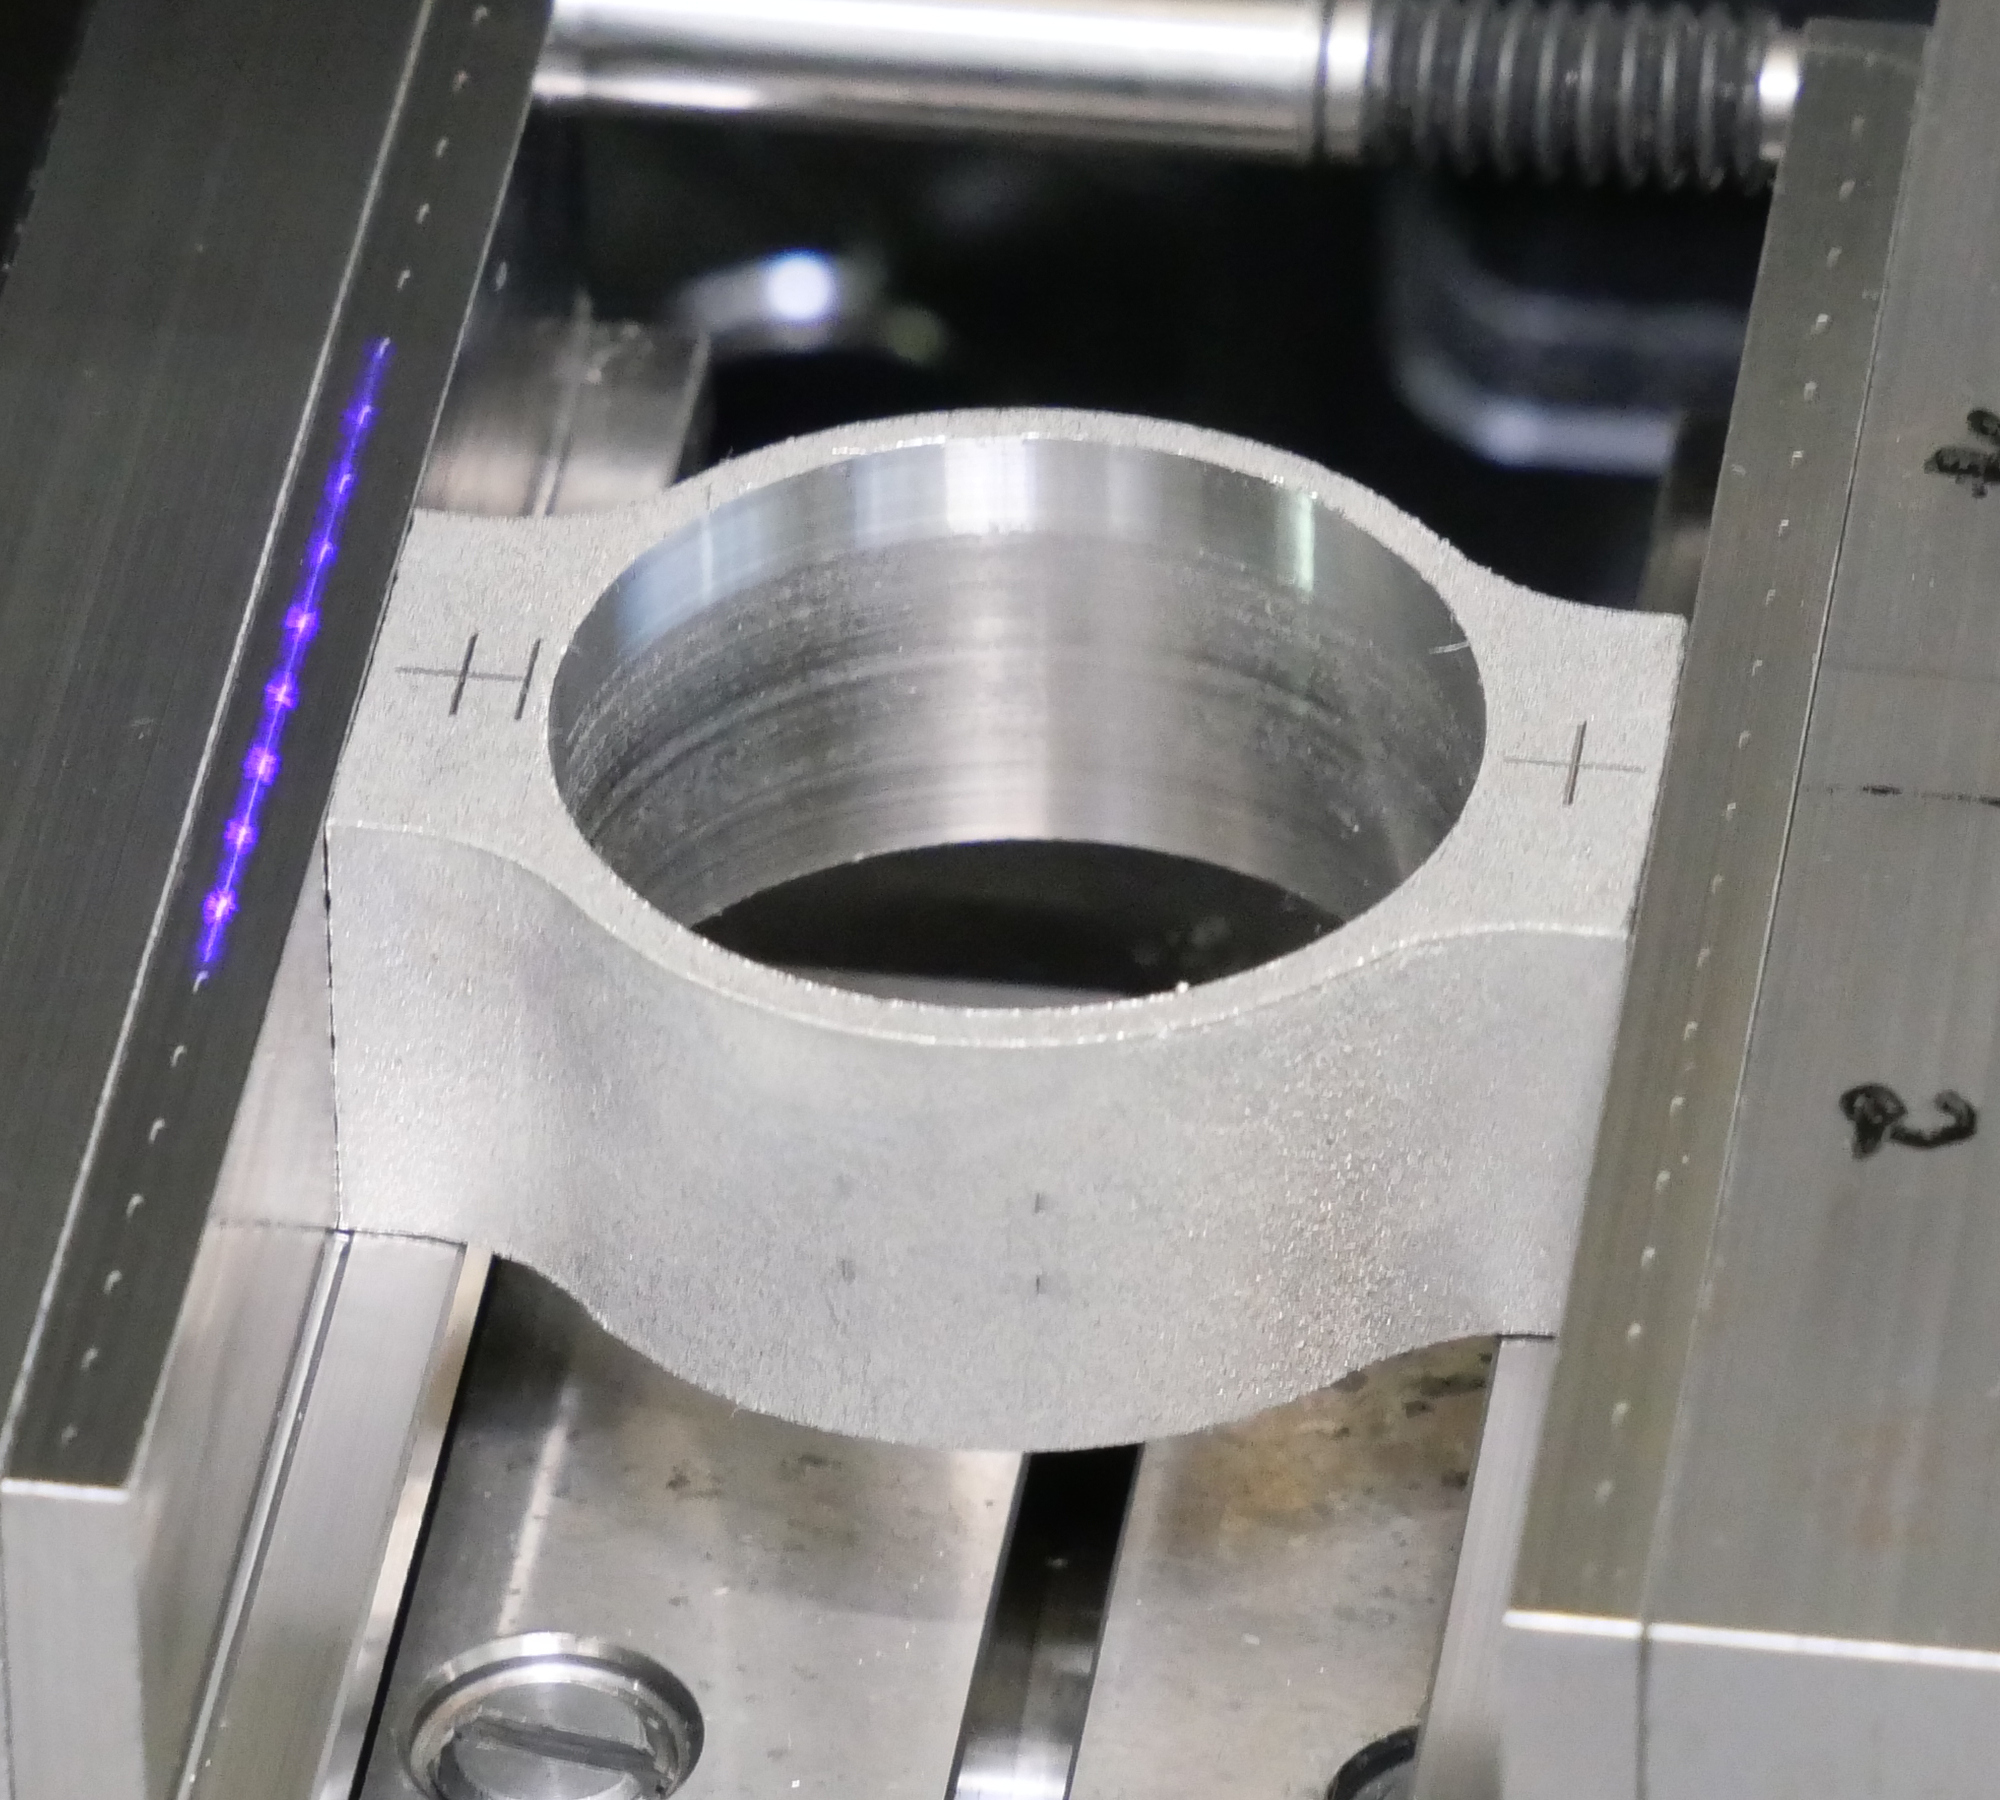
\includegraphics[width=0.9\linewidth]{images/AM2_crop.JPG}
        \caption*{(c)}
      \end{minipage}
      \caption{(a): AF Metallbauteil mit voller Stützstruktur, Bezeichnung: AM0.
      (b): AF Bauteil mit der halben Stützstruktur ausgebohrt, Bezeichnung: AM1.
      (c): AF Bauteil ohne Stützstruktur, Bezeichnung: AM2}
      \label{fig:am_parts}
\end{figure}

\section{Ergebnisse der optischen Deformationsanalyse}

In Abbildung \ref{fig:am_defos} und Abbildung \ref{fig:fdm_defos} sind die erkannten,
vertikalen Deformation grafisch dargestellt. Jeweils von Spannungsstufe null bis 
Spannungsstufen Sechs. Bei dem FDM Bauteil fehlt die Spannungsstufen fünf, 
diese ist leider bei der händischen Dateiname Vergabe überschrieben worden und konnte 
deshalb nicht ausgewertet worden. Aus diesem Grund ist eine so große Lücke in der 
Abbildung \ref{fig:fdm_defos}.
Außerdem sind große Unterschiede in der absoluten Deformation zu sehen. Zum Beispiel 
die rote Kurve in Abbildung \ref{fig:am_defos} die den Unterschied der Spannungsstufen 
null und eins angibt. Diese Kurve sollte näher an null der y-Achse liegen. 
Dies liegt an Ungenauigkeiten in dem Stitching Verfahren. In den Graphen ist also 
auf die Steigung der Deformationskurve zu achten. In der Steigung erkannt man das 
sich die Bauteile in mittleren Bereich nach außen hin deformiert haben und in 
den Randbereichen sich nach innen und dann wieder nach außen deformieren.
Außerdem ist im Vergleich der beiden Graphen zu sehen das sich das FDM Bauteil deutlich 
mehr verformt hat. Hier beträgt die größte Deformation über 150 Pixel.
Bei dem Metallbauteil, das mit der zehnfachen Kraft eingespannt wurde (250 nm vs. 2500 nm)
sind es nur knapp 40 Pixel, wie in Abbildung~\ref{fig:deformation_data_am} zu sehen. Trotzdem ist zu sehen das sich die Bauteile, die auch die 
gleiche Geometrie teilen, auf die gleiche Weise verformt haben.

\begin{figure}[H]
  \centering
  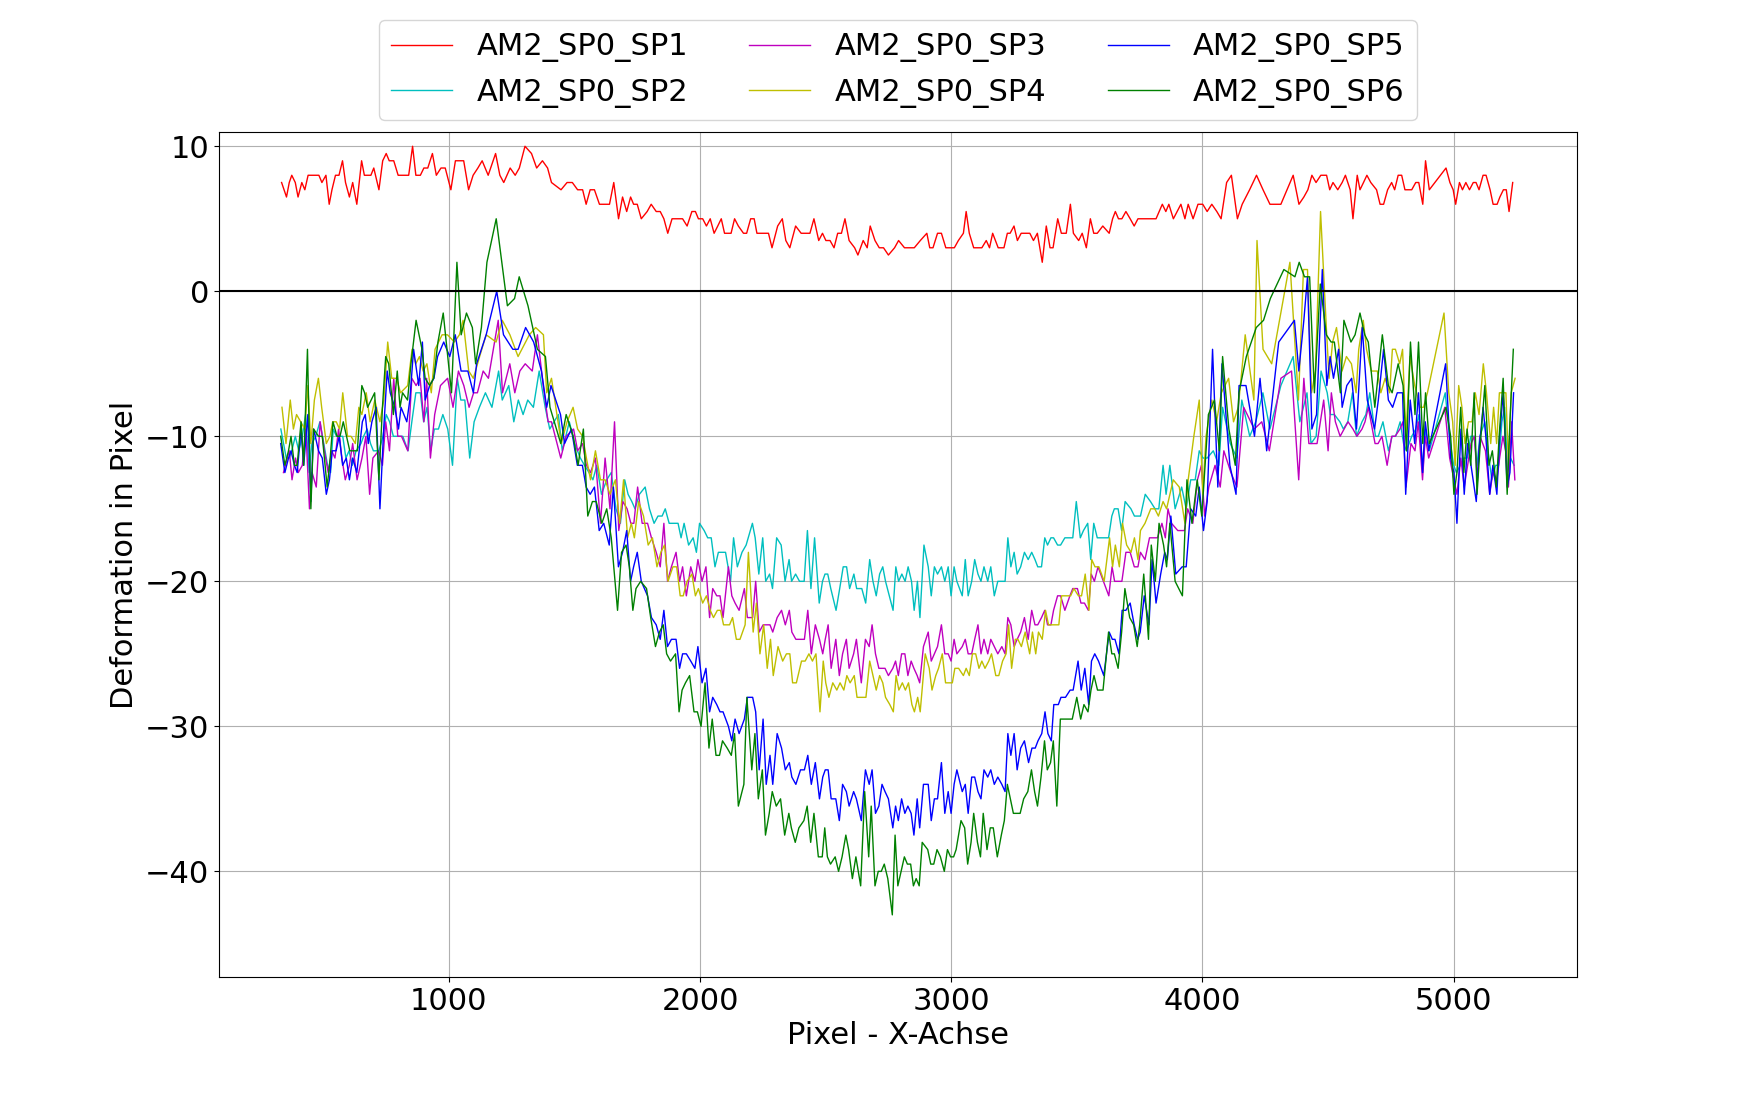
\includegraphics[width=0.95\textwidth]{images/am2_all_defos.png}
  \caption{Sechs Deformationsstufen bei einem additiv gefertigten Metallbauteil ohne
  Stützstruktur von 0 bis 2500 nm}
  \label{fig:am_defos}
\end{figure}

\begin{figure}[H]
  \centering
  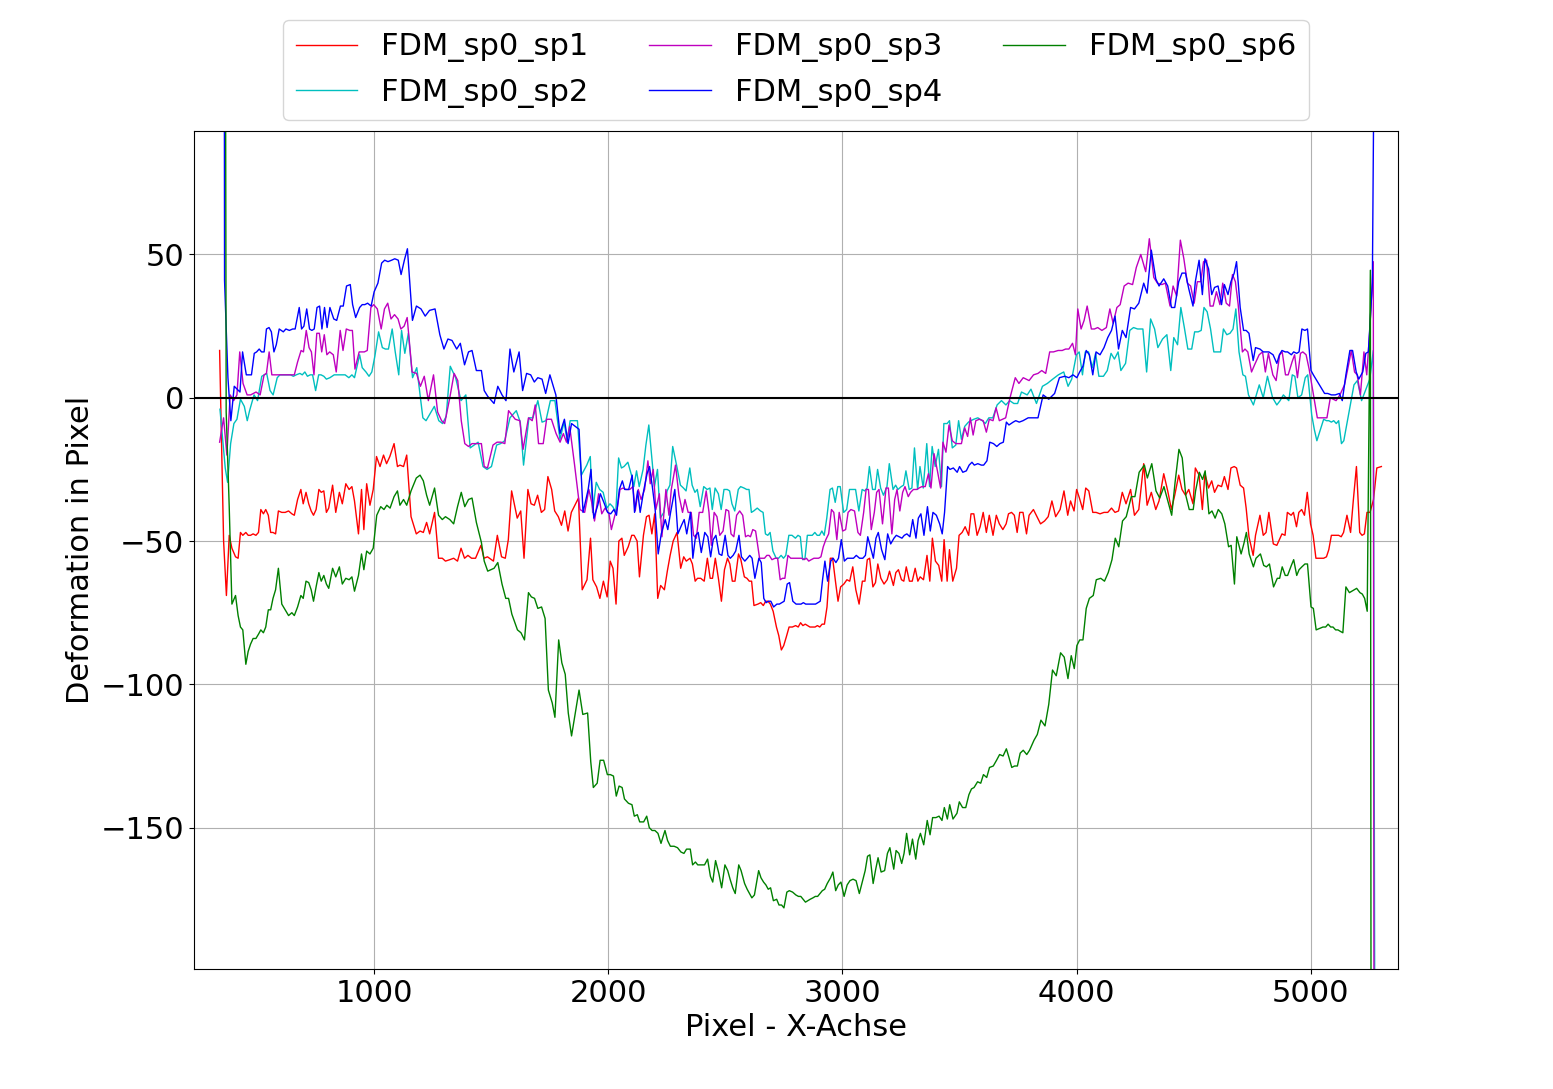
\includegraphics[width=0.95\textwidth]{images/fdm2_all_defos.png}
  \caption{Fünf Deformationsstufen bei einem FDM Bauteil von 0 bis 250 nm}
  \label{fig:fdm_defos}
\end{figure}

\begin{figure}[H]
    \centering
    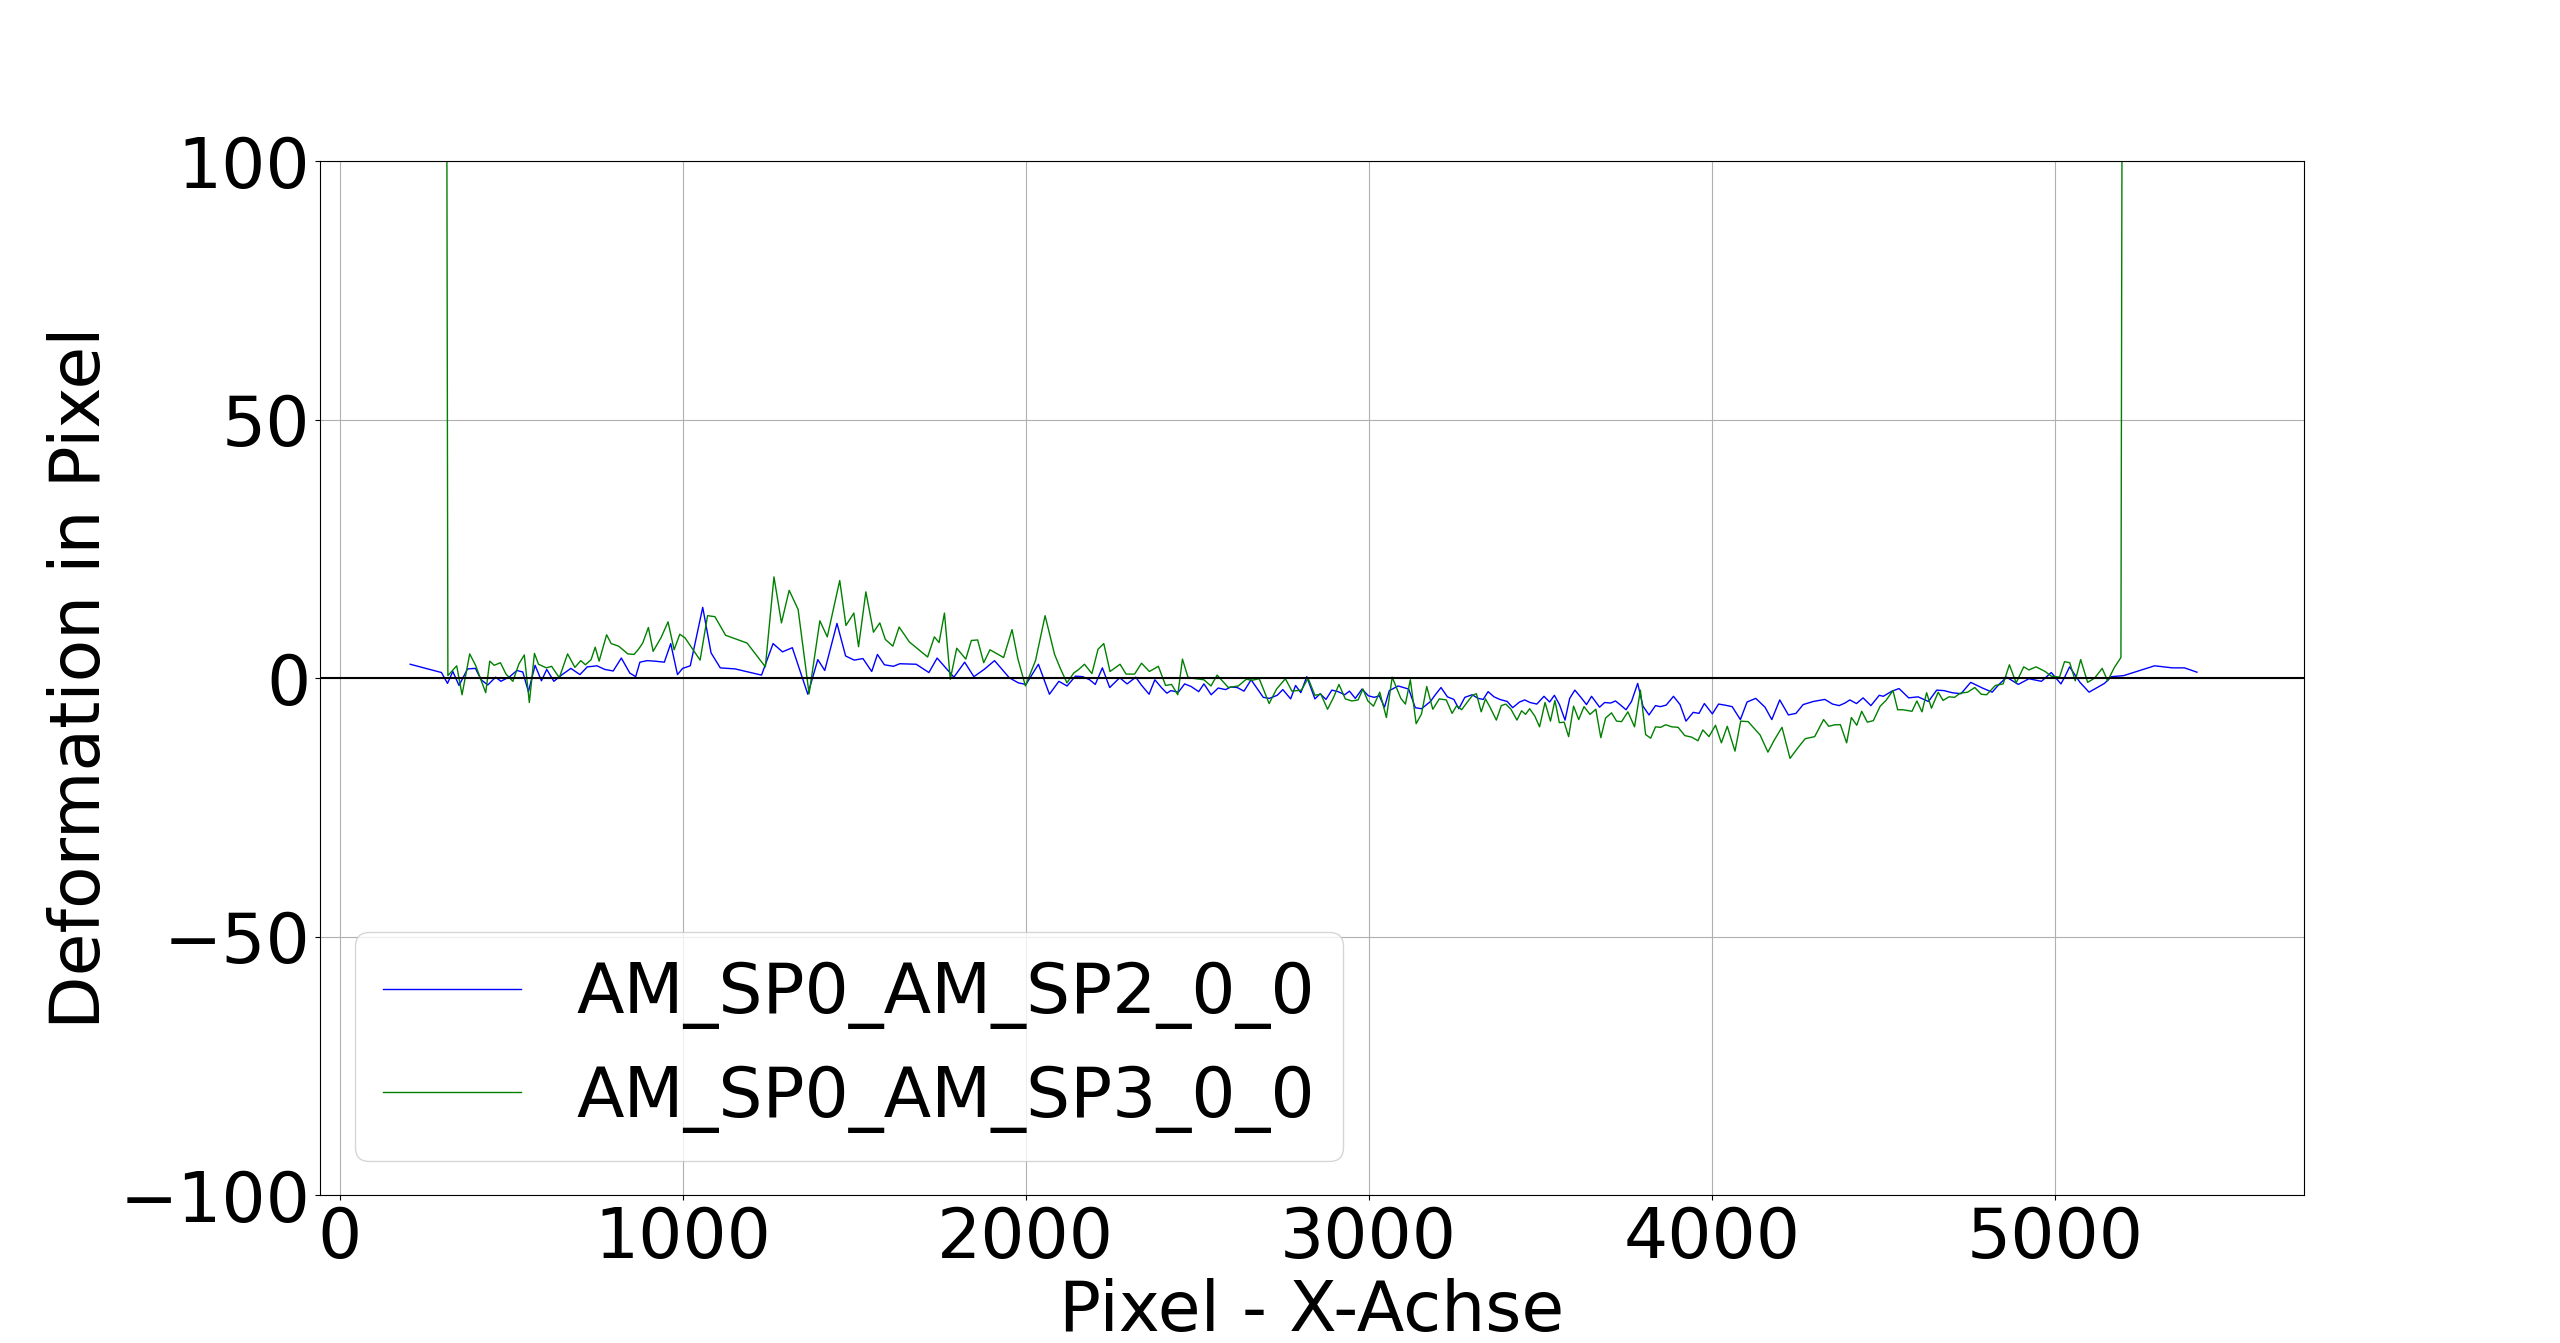
\includegraphics[width=0.9\textwidth]{images/AM_sp0_sp2_defo_plot.png}
    \caption{Differenz von zwei Spannungsstufen bei einem additiv gefertigten Metallbauteil, 
    das zur Hälfte mit Stützstrukturen gefüllt ist (Abbildung~\ref{fig:am_parts (b)}). }
    \label{fig:deformation_data_am}
\end{figure}

\section{Beurteilung der Ergebnisse}

Grundsätzlich ermöglicht die Methode die Erkennung und den Vergleich von Deformationen 
eines Bauteils. Die gemessene Deformation eines Bauteils entspricht den erwarteten Werten, 
abhängig von Material und Geometrie des Bauteils. FDM-gedruckte Kunststoffteile zeigen 
eine deutlich stärkere Verformung im Vergleich zu Metallteilen.
Bei den Metallteilen zeigt sich, dass das Vorhandensein einer Stützstruktur die
Verformung des Bauteils signifikant reduziert. 
Die unterschiedlichen Deformationen sind in Abbildung \ref{fig:materials} dargestellt. 
Das in Abbildung \ref{fig:am_parts} (a) gezeigte Bauteil konnte nicht analysiert werden, 
da durch die Stützstruktur keine korrekte Transformation zur stitchen berechnet werden konnte.
Bei den FDM-Bauteilen ist festzustellen, dass sie sich deutlich stärker verformen 
als die Metallteile. Beide FDM-Bauteile zeigen eine ähnliche Verformungsausprägung, 
jedoch tritt die Deformation, trotz identischer Geometrie, an unterschiedlichen Stellen auf. 
Dies könnte auf Unterschiede im Druckprozess zurückzuführen sein. 
Diese Beobachtung zeigt einen weiteren Nutzen der Methodik: Sie ermöglicht
nicht nur die Bestimmung des Ausmaßes der Deformation, sondern auch die 
Identifikation von Schwachstellen innerhalb eines Bauteils, die zu einer erhöhten 
 
Deformation führen.

\begin{figure}[H]
  \centering
  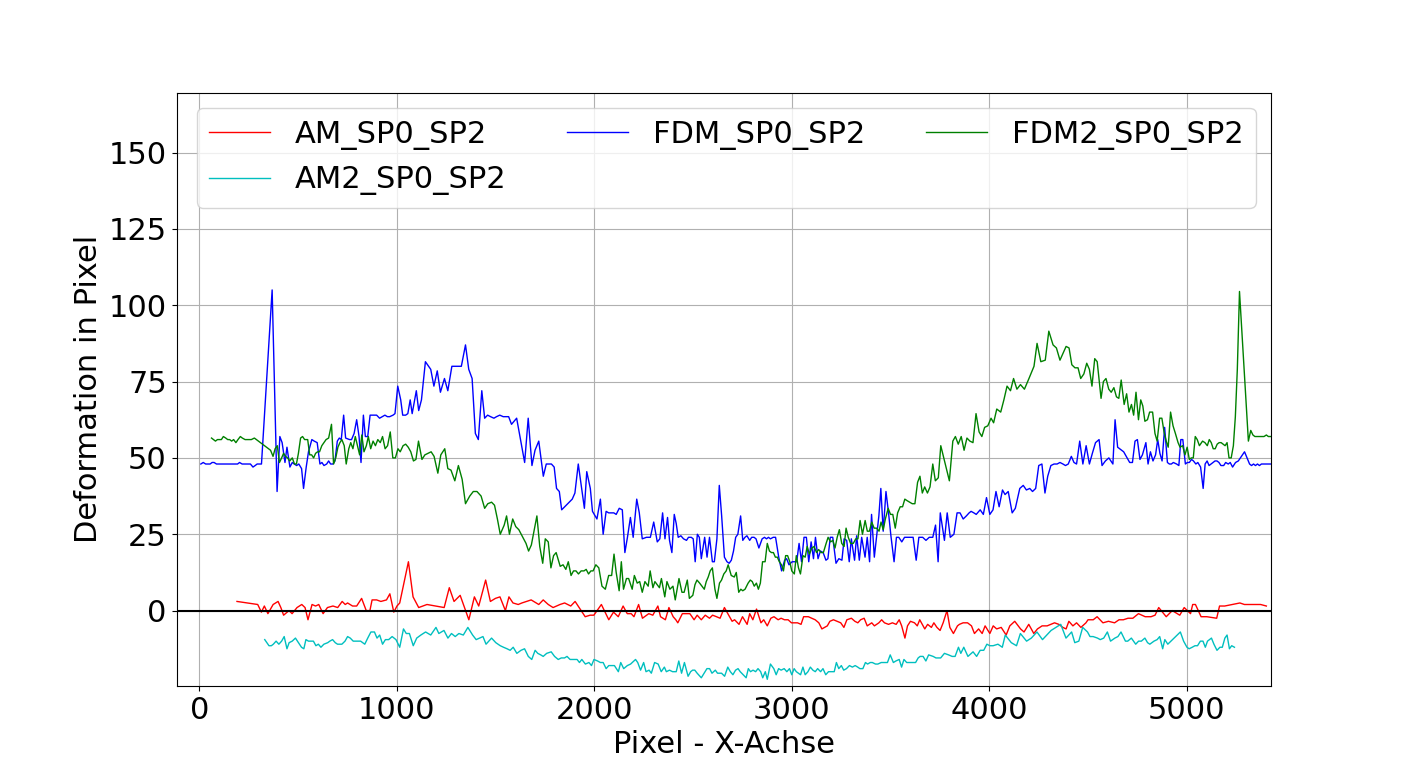
\includegraphics[width=0.95\textwidth]{images/compare_materials.png}
  \caption{Vergleich von Materialien und Bauteilgeometrien}
  \label{fig:materials}
\end{figure}

Dennoch ist die Deformationserkennung noch nicht perfekt. 
Fehler im Stitching Prozess führen zu starken Änderungen in der Deformationserkennung. 
Wie in Abbildung \ref{fig:errors} zu sehen ist, kann sich die Breite des Bauteils 
zwischen zwei Spannungsstufen unterscheiden. Er ist erkennbar, dass der Rand der einen 
Kontur, repräsentiert durch die magenta gefärbte Linie, immer größer ist als 
der Rand der anderen Kontur, hier in blau dargestellt.
Dieser Versatz entsteht, weil beim Stitching eine Transformation verwendet wurde die sich 
um wenige Pixel unterscheidet. Dadurch wächst auch die erkannte Deformationen.
Aus diesem Grund existieren in den Abbildungen \ref{fig:am_defos} und \ref{fig:fdm_defos}
Linien die nicht dem erwarteten Verhalten entsprechen. 
In Abbildung \ref{fig:fdm_defos} zum Beispiel, sollte die Deformation zwischen den 
Spannungsstufen eins und zwei 
(in rot dargestellt) am kleinsten sein. Stattdessen liegt die Kurve bei -50 Pixeln im Graph.

\begin{figure}[H]
  \centering
  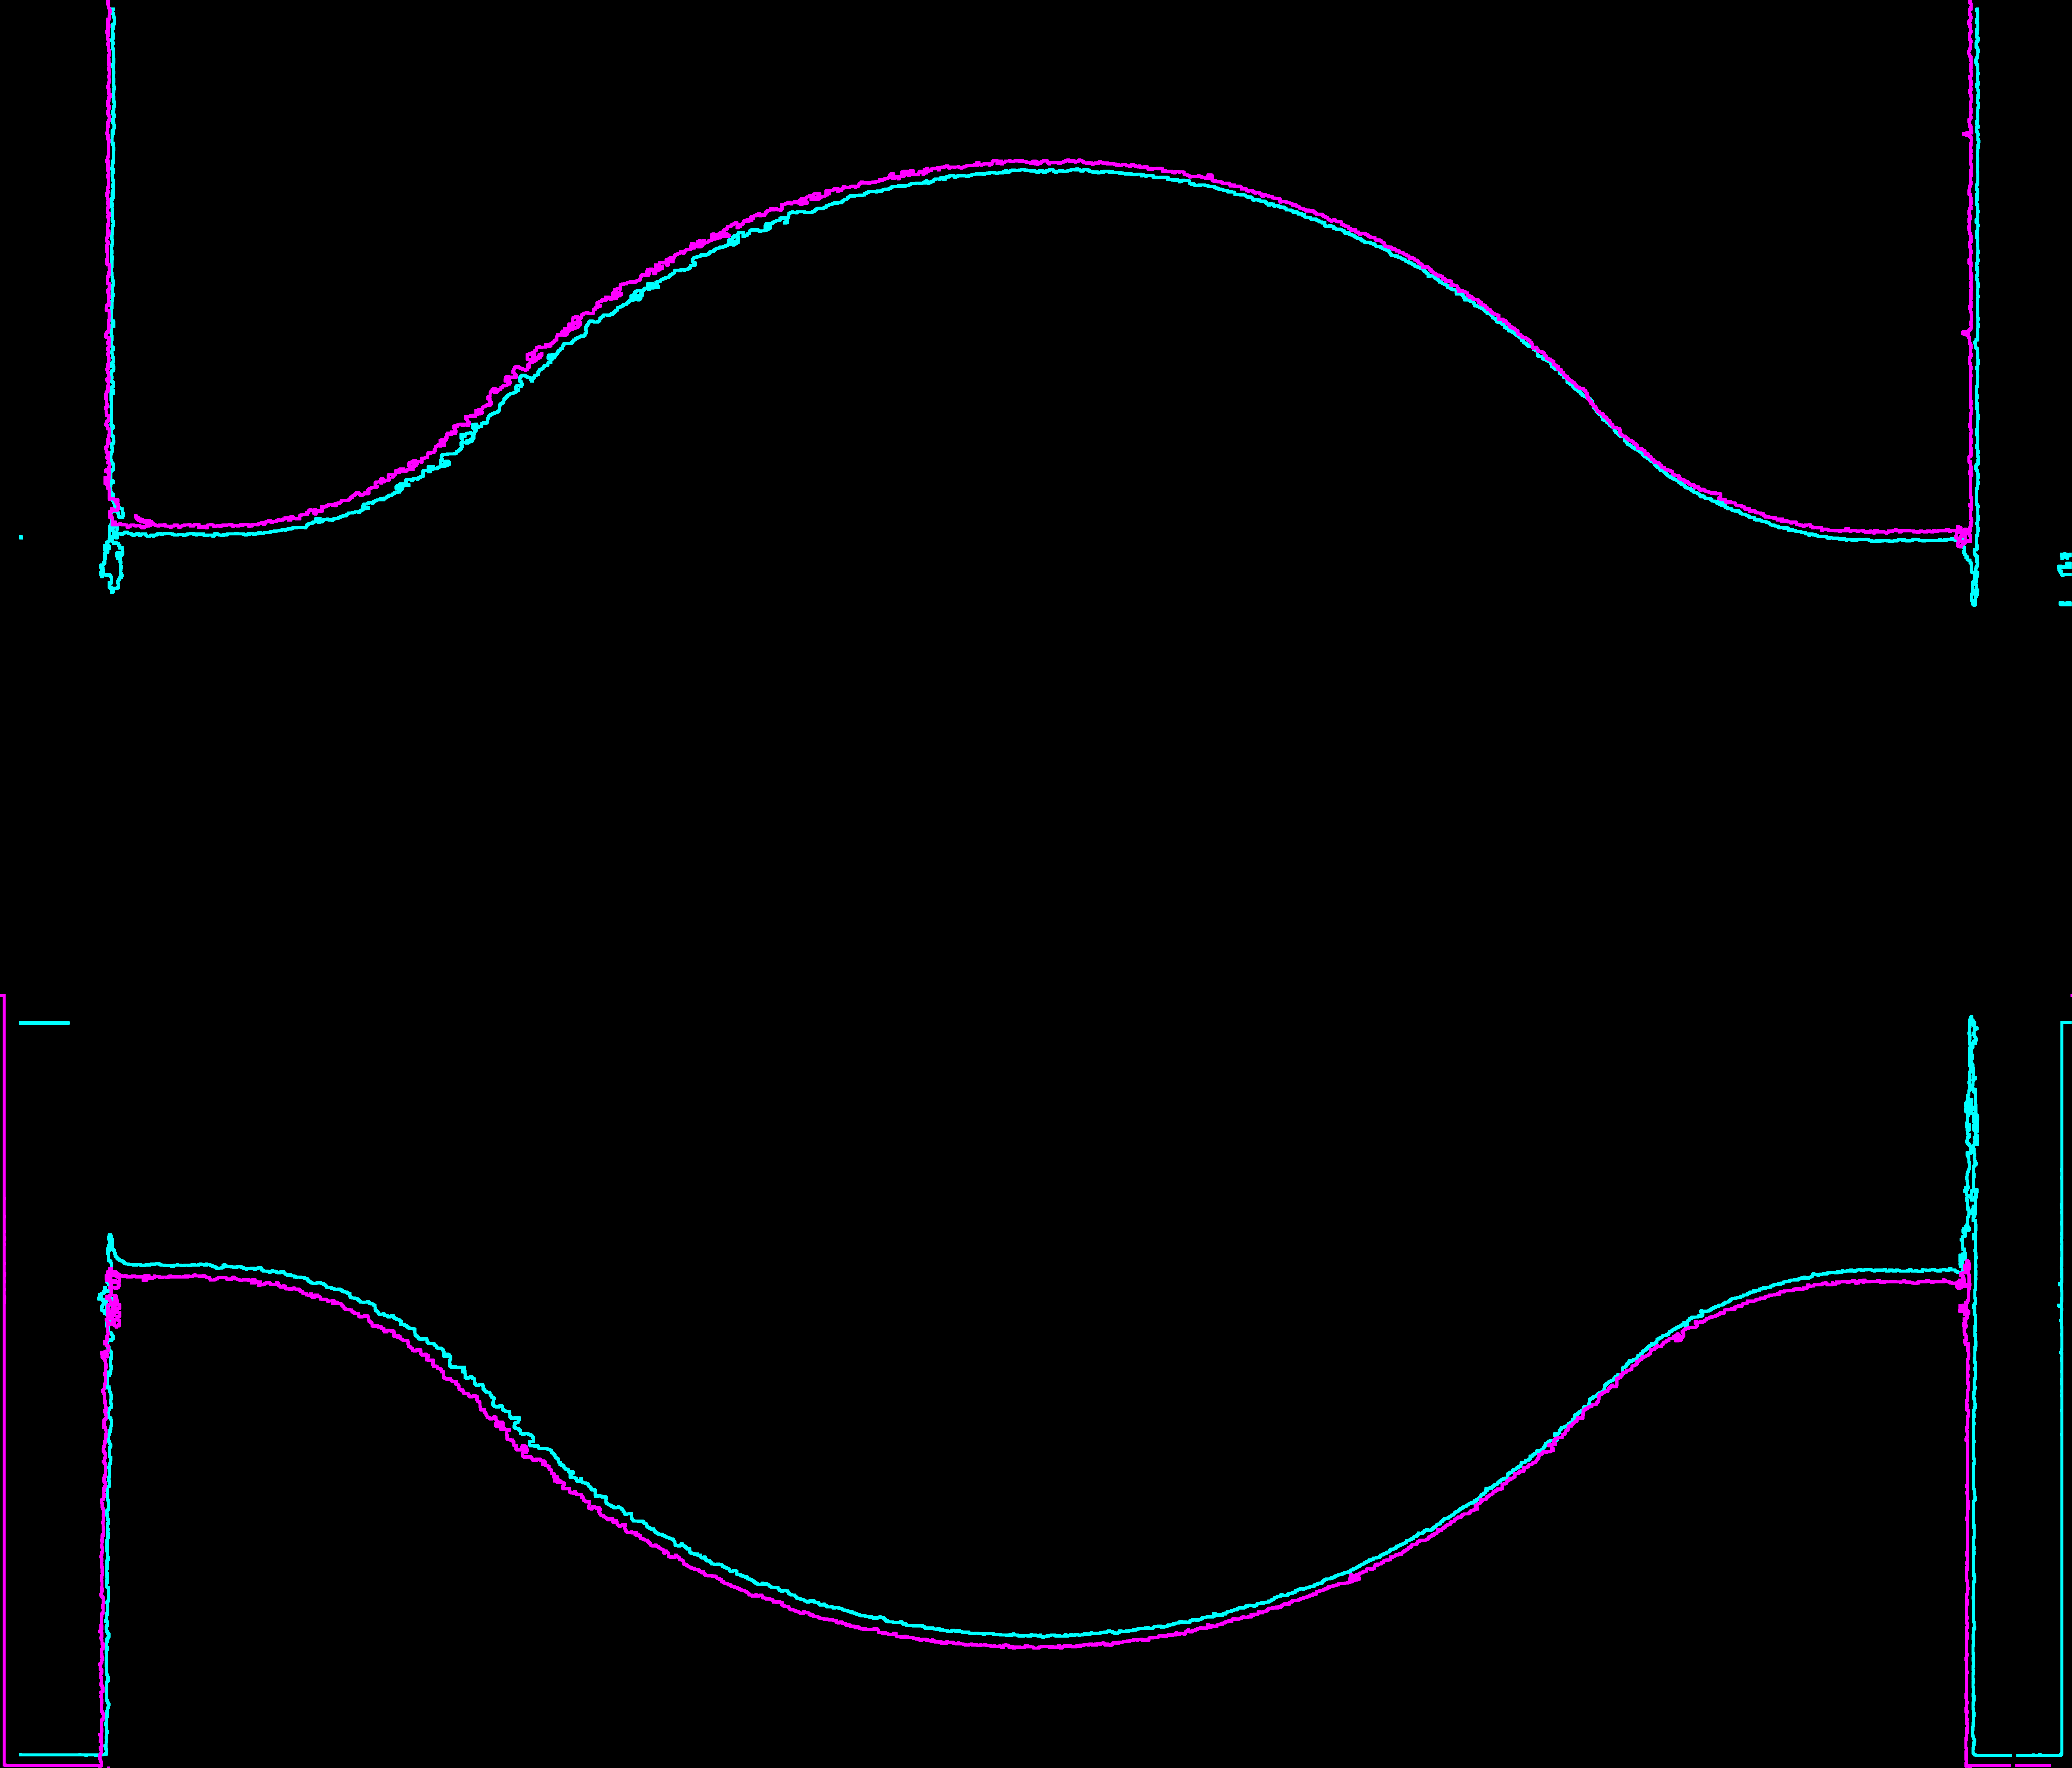
\includegraphics[width=0.95\textwidth]{images/contours_matching_36.png}
  \caption{Vergleich von Konturen aus nicht korrekt zusammengefügten Bildern.}
  \label{fig:errors}
\end{figure}

Zusätzlich kann, bei Bildern ohne klare Konturen, das Stitching nicht korrekt durchgeführt
werden. Dies ist bei den additiv gefertigten Metallbauteil mit Stützstruktur der Fall 
(Abbildung \ref{fig:am_parts} (a)). Das Bild, das aus dem Scan dieses Bauteils erstellt wurde, 
ist in Abbildung \ref{fig:errorimage} zu sehen. Es lassen sich keine eindeutigen Konturen 
erkennen, die für das Stitching genutzt werden könnten.

\begin{figure}[H]
  \centering
  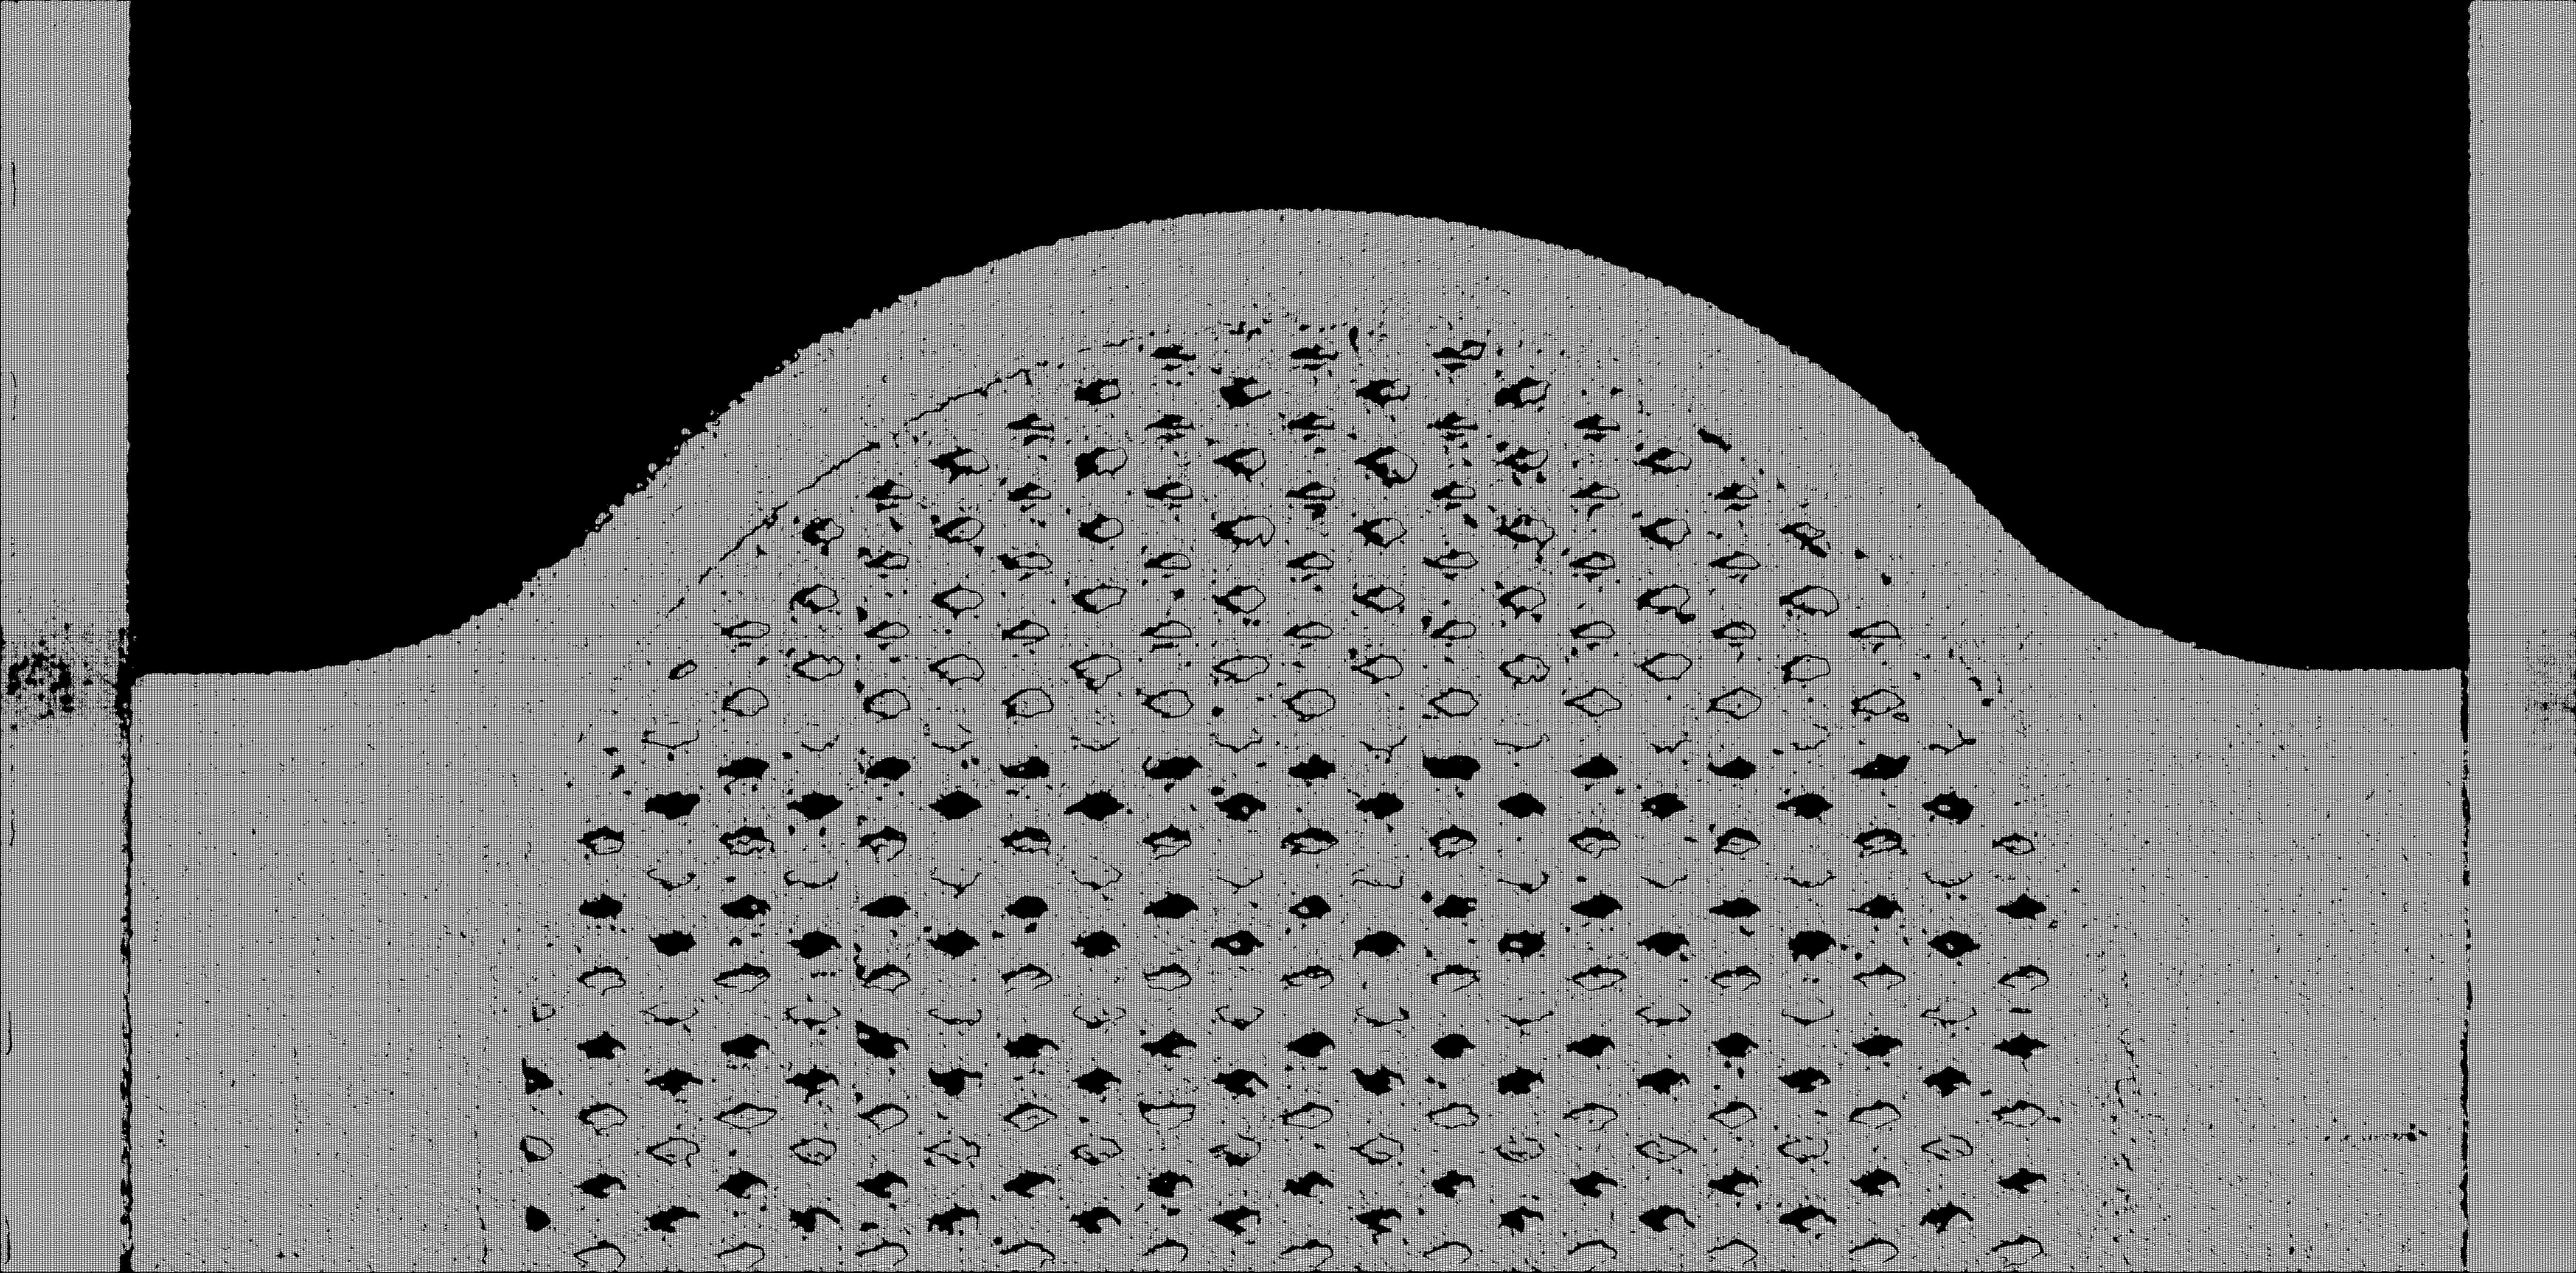
\includegraphics[width=0.95\textwidth]{images/am0.png}
  \caption{Bild eines Scans von einem Metallbauteil mit Stützstruktur.}
  \label{fig:errorimage}
\end{figure}




\newpage
\bibliography{quellen}
\bibliographystyle{alpha}

\end{document}